
%%%%%%%%%%%%%%%%%%%%%%%%%%%%%%%%%%%%%%%%%%%%%%%%%%%%%%%%%%%%%%%%%%%%%%%%%%%%%%%%
%% ************************************************************************** %%
%% *                                Settings                                * %%
%% ************************************************************************** %%
%%%%%%%%%%%%%%%%%%%%%%%%%%%%%%%%%%%%%%%%%%%%%%%%%%%%%%%%%%%%%%%%%%%%%%%%%%%%%%%%
\documentclass{tron}
\loadglsentries{gls}
\glsaddall
\addbibresource{reference}
\usepackage{xcolor}  % Coloured text etc.
\usepackage{float}
% fancy note style
% additional fancy boxes
\usepackage[framemethod=TikZ]{mdframed}
%\usepackage{amsthm}

% gray color indicates [OPTIONAL READING]

%%%%%%%%%%%%%%%%%%%%%%%%%%%%%%
%Note
\newenvironment{note}[3][]{%
	\ifstrempty{#1}%
	{\mdfsetup{%
	frametitle={%
	\tikz[baseline=(current bounding box.east),outer sep=0pt]
	\node[anchor=east,rectangle,fill=#2]
	{\strut Note};}}
	}%
	{\mdfsetup{%
	frametitle={%
	\tikz[baseline=(current bounding box.east),outer sep=0pt]
	\node[anchor=east,rectangle,fill=#2]
	{\strut #1};}}%
	}%
	\mdfsetup{innertopmargin=0pt,skipabove=5pt,linecolor=#2,%
		linewidth=2pt,topline=true,%
		frametitleaboveskip=\dimexpr-\ht\strutbox\relax,
		backgroundcolor={white!90!#2}}
	\begin{mdframed}[]\relax%
	\label{#3}}{\end{mdframed}
}

\newcommand{\createnoteenv}[6]{
	\refstepcounter{#6}%
	\ifstrempty{#1}%
	{\mdfsetup{%
	frametitle={%
	\tikz[baseline=(current bounding box.east),outer sep=0pt]
	\node[anchor=east,rectangle,fill=#3]
	{\strut #4~#5};}}
	}%
	{
		\mdfsetup{%
			frametitle={%
				\tikz[baseline=(current bounding box.east),outer sep=0pt]
				\node[anchor=east,rectangle,fill=#3]
				{\strut #4~#5:~#1};
			}
		}%
	}%
	\mdfsetup{innertopmargin=0pt,skipabove=5pt,linecolor=#3,%
	linewidth=2pt,topline=true,%
	frametitleaboveskip=\dimexpr-\ht\strutbox\relax}
	\begin{mdframed}[]\relax%
	\label{#2}
}

\newcommand{\createnoteenvback}[6]{
	\refstepcounter{#6}%
	\ifstrempty{#1}%
	{\mdfsetup{%
	frametitle={%
	\tikz[baseline=(current bounding box.east),outer sep=0pt]
	\node[anchor=east,rectangle,fill=#3]
	{\strut #4~#5};}}
	}%
	{
		\mdfsetup{%
			frametitle={%
				\tikz[baseline=(current bounding box.east),outer sep=0pt]
				\node[anchor=east,rectangle,fill=#3]
				{\strut #4~#5:~#1};
			}
		}%
	}%
	\mdfsetup{innertopmargin=0pt,skipabove=5pt,linecolor=#3,%
	linewidth=2pt,topline=true,%
	frametitleaboveskip=\dimexpr-\ht\strutbox\relax,
	backgroundcolor={white!90!#3}}
	\begin{mdframed}[]\relax%
	\label{#2}
}

%%%%%%%%%%%%%%%%%%%%%%%%%%%%%%
%Pro
\newcounter{pros}[chapter] \setcounter{pros}{0}
\renewcommand{\thepros}{\arabic{chapter}.\arabic{section}.\arabic{pros}}
\newenvironment{pros}[2][]{%
	\createnoteenv{#1}{#2}{green!40!white}{Pros}{\thepros}{pros}%
}{\end{mdframed}}

%%%%%%%%%%%%%%%%%%%%%%%%%%%%%%
%Con
\newcounter{cons}[chapter] \setcounter{cons}{0}
\renewcommand{\thecons}{\arabic{chapter}.\arabic{section}.\arabic{cons}}
\newenvironment{cons}[2][]{%
	\createnoteenv{#1}{#2}{red!40!white}{Cons}{\thecons}{cons}%
}{\end{mdframed}}

%%%%%%%%%%%%%%%%%%%%%%%%%%%%%%
%Definition
\newcounter{definition}[chapter] \setcounter{definition}{0}
\renewcommand{\thedefinition}{\arabic{chapter}.\arabic{section}.\arabic{definition}}
\newenvironment{definition}[2][]{%
	\createnoteenv{#1}{#2}{blue!40}{Definition}{\thedefinition}{definition}%
}{\end{mdframed}}

%%%%%%%%%%%%%%%%%%%%%%%%%%%%%%
%overview
\newcounter{overview}[chapter] \setcounter{overview}{0}
\renewcommand{\theoverview}{\arabic{chapter}.\arabic{section}.\arabic{overview}}
\newenvironment{overview}[2][]{%
	\createnoteenv{#1}{#2}{blue!30!cyan}{Overview}{\theoverview}{overview}%
}{\end{mdframed}}

%%%%%%%%%%%%%%%%%%%%%%%%%%%%%%
%theoremrem
\newcounter{theorem}[chapter] \setcounter{theorem}{0}
\renewcommand{\thetheorem}{\arabic{chapter}.\arabic{section}.\arabic{theorem}}
\newenvironment{theorem}[2][]{%
	\createnoteenv{#1}{#2}{cyan!40}{Theorem}{\thetheorem}{theorem}%
}{\end{mdframed}}


%%%%%%%%%%%%%%%%%%%%%%%%%%%%%%
%Proof
\newcounter{proof}[chapter]\setcounter{proof}{0}
\renewcommand{\theproof}{\arabic{chapter}.\arabic{section}.\arabic{proof}}
\newenvironment{proof}[2][]{%
	\createnoteenv{#1}{#2}{red!20}{Proof}{\theproof}{proof}%
}{\end{mdframed}}

%%%%%%%%%%%%%%%%%%%%%%%%%%%%%%
%Alert
\newcounter{alert}[chapter]\setcounter{alert}{0}
\renewcommand{\thealert}{\arabic{chapter}.\arabic{section}.\arabic{alert}}
\newenvironment{alert}[2][]{%
	\createnoteenv{#1}{#2}{red!80}{Alert}{\thealert}{alert}%
}{\end{mdframed}}

%%%%%%%%%%%%%%%%%%%%%%%%%%%%%%
%Remark
\newcounter{remark}[chapter]\setcounter{remark}{0}
\renewcommand{\theremark}{\arabic{chapter}.\arabic{section}.\arabic{remark}}
\newenvironment{remark}[2][]{%
	\createnoteenv{#1}{#2}{orange!40}{Remark}{\theremark}{remark}%
}{\end{mdframed}}

%%%%%%%%%%%%%%%%%%%%%%%%%%%%%%
%Exercise
\newcounter{exercise}[chapter]\setcounter{exercise}{0}
\renewcommand{\theexercise}{\arabic{chapter}.\arabic{section}.\arabic{exercise}}
\newenvironment{exercise}[2][]{%
	\createnoteenv{#1}{#2}{purple!40}{Exercise}{\theexercise}{exercise}%
}{\end{mdframed}}

%%%%%%%%%%%%%%%%%%%%%%%%%%%%%%
%Example
\newcounter{example}[chapter]\setcounter{example}{0}
\renewcommand{\theexample}{\arabic{chapter}.\arabic{section}.\arabic{example}}
\newenvironment{example}[2][]{%
	\createnoteenv{#1}{#2}{blue!40!cyan!20}{Example}{\theexample}{example}%
}{\end{mdframed}}

%%%%%%%%%%%%%%%%%%%%%%%%%%%%%%
%Algorithm
\newcounter{algo}[chapter]\setcounter{algo}{0}
\renewcommand{\thealgo}{\arabic{chapter}.\arabic{section}.\arabic{algo}}
\newenvironment{algo}[2][]{%
	\createnoteenv{#1}{#2}{yellow!90!brown!60}{Algorithm}{\thealgo}{algo}%
}{\end{mdframed}}

%%%%%%%%%%%%%%%%%%%%%%%%%%%%%%
%EQN
\newcounter{eqn}[chapter]\setcounter{eqn}{0}
\renewcommand{\theeqn}{\arabic{chapter}.\arabic{section}.\arabic{eqn}}
\newenvironment{eqn}[2][]{%
	\createnoteenvback{#1}{#2}{red!20!white}{Equation}{\theeqn}{eqn}%
	\begin{equation}
}{\end{equation}\end{mdframed}}


%%%%%%%%%%%%%%%%%%%%%%%%%%%%%%
\newcommand{\red}[1]{\textcolor{red}{#1}}
\newcommand{\blue}[1]{\textcolor{blue}{#1}}

%%%%%%%%%%%%%%%%%%%%%%%%%%%%%%
%Examples
% {

%     \subsection{Theorem and lemma examples with title}
%     \begin{theorem}[Pythagoras' theorem]{theorem:pythagoras}
%     In a right triangle, the square of the hypotenuse is equal to the sum of the squares of the catheti.
%     \[a^2+b^2=c^2\]
%     \end{theorem}
%     In mathematics, the Pythagorean theorem, also known as Pythagoras' theorem (see theorem \ref{theorem:pythagoras}), is a relation in Euclidean geometry among the three sides of a right triangle.
%     
%     \begin{definition}[B\'ezout's identity]{def:bezout}
%     Let $a$ and $b$ be nonzero integers and let $d$ be their greatest common divisor. Then there exist integers $x$ and $y$ such that:
%     \[ax+by=d\]
%     \end{definition}
%     This is a reference to Bezout's lemma \ref{def:bezout}
%     
%     
%     \subsection{Theorem and proof examples without title}
%     
%     \begin{theorem}[]{theorem:theorem1}
%     There exist two irrational numbers $x$, $y$ such that $x^y$ is rational.
%     \end{theorem}
%     
%     \begin{proof}[]{proof:proof1}
%     If $x=y=\sqrt{2}$ is an example, then we are done; otherwise $\sqrt{2}^{\sqrt{2}}$ is irrational, in which case taking $x=\sqrt{2}^{\sqrt{2}}$ and $y=\sqrt{2}$ gives us:
%     \[\bigg(\sqrt{2}^{\sqrt{2}}\bigg)^{\sqrt{2}}=\sqrt{2}^{\sqrt{2}\sqrt{2}}=\sqrt{2}^{2}=2.\]
%     \end{proof}
%
%     \begin{alert}[]{alert:alert1}
%     If $x=y=\sqrt{2}$ is an example, then we are done; otherwise $\sqrt{2}^{\sqrt{2}}$ is irrational, in which case taking $x=\sqrt{2}^{\sqrt{2}}$ and $y=\sqrt{2}$ gives us:
%     \[\bigg(\sqrt{2}^{\sqrt{2}}\bigg)^{\sqrt{2}}=\sqrt{2}^{\sqrt{2}\sqrt{2}}=\sqrt{2}^{2}=2.\]
%     \end{alert}
%     
%     \begin{remark}[]{alert:alert1}
%     If $x=y=\sqrt{2}$ is an example, then we are done; otherwise $\sqrt{2}^{\sqrt{2}}$ is irrational, in which case taking $x=\sqrt{2}^{\sqrt{2}}$ and $y=\sqrt{2}$ gives us:
%     \[\bigg(\sqrt{2}^{\sqrt{2}}\bigg)^{\sqrt{2}}=\sqrt{2}^{\sqrt{2}\sqrt{2}}=\sqrt{2}^{2}=2.\]
%     \end{remark}
%     
%     
%          \begin{exercise}[]{alert:alert1}
%     If $x=y=\sqrt{2}$ is an example, then we are done; otherwise $\sqrt{2}^{\sqrt{2}}$ is irrational, in which case taking $x=\sqrt{2}^{\sqrt{2}}$ and $y=\sqrt{2}$ gives us:
%     \[\bigg(\sqrt{2}^{\sqrt{2}}\bigg)^{\sqrt{2}}=\sqrt{2}^{\sqrt{2}\sqrt{2}}=\sqrt{2}^{2}=2.\]
%     \end{exercise}
%     
%     \begin{algo}[]{algorithm:alert1}
%     If $x=y=\sqrt{2}$ is an example, then we are done; otherwise $\sqrt{2}^{\sqrt{2}}$ is irrational, in which case taking $x=\sqrt{2}^{\sqrt{2}}$ and $y=\sqrt{2}$ gives us:
%     \[\bigg(\sqrt{2}^{\sqrt{2}}\bigg)^{\sqrt{2}}=\sqrt{2}^{\sqrt{2}\sqrt{2}}=\sqrt{2}^{2}=2.\]
%     \end{algo}
%     
%     \begin{note}[Goal]{pink}{note:goal}
%     If $x=y=\sqrt{2}$ is an example, then we are done; otherwise $\sqrt{2}^{\sqrt{2}}$ is irrational, in which case taking $x=\sqrt{2}^{\sqrt{2}}$ and $y=\sqrt{2}$ gives us:
%     \[\bigg(\sqrt{2}^{\sqrt{2}}\bigg)^{\sqrt{2}}=\sqrt{2}^{\sqrt{2}\sqrt{2}}=\sqrt{2}^{2}=2.\]
%     \end{note}

% }
%\usepackage{lipsum}                     % Dummytext
\usepackage{xargs}                      % Use more than one optional parameter in a new commands
\usepackage[colorinlistoftodos,prependcaption,textsize=normalsize]{todonotes}
%
\newcommandx{\unsure}[2][1=]{\todo[linecolor=red,backgroundcolor=red!25,bordercolor=red,#1]{#2}}
\newcommandx{\change}[2][1=]{\todo[linecolor=blue,backgroundcolor=blue!25,bordercolor=blue,#1]{#2}}
\newcommandx{\info}[2][1=]{\todo[linecolor=OliveGreen,backgroundcolor=OliveGreen!25,bordercolor=OliveGreen,#1]{#2}}
\newcommandx{\improvement}[2][1=]{\todo[linecolor=Plum,backgroundcolor=Plum!25,bordercolor=Plum,#1]{#2}}
\newcommandx{\thiswillnotshow}[2][1=]{\todo[disable,#1]{#2}}
%
\preto\printlistoftodos{
    \listoftodos[Todo List]
}

% EXAMPLES:
    % \todo[inline]{The original todo note withouth changed colours.\newline Here's another line.}
    % \lipsum[11]\unsure{Is this correct?}\unsure{I'm unsure about also!}
    % \lipsum[11]\change{Change this!}
    % \lipsum[11]\info{This can help me in chapter seven!}
    % \lipsum[11]\improvement{This really needs to be improved!\newline\newline What was I thinking?!}
    % \lipsum[11]
    % \thiswillnotshow{This is hidden since option `disable' is chosen!}
    % \improvement[inline]{The following section needs to be rewritten!}
    % \lipsum[11]
    % \newpage
    % \listoftodos[Notes]
%%%  Equation Condition
\newenvironment{eqconditions}
  {\par\vspace{\abovedisplayskip}\noindent\begin{tabular}{>{$}l<{$} @{${}={}$} l}}
  {\end{tabular}\par\vspace{\belowdisplayskip}}
\newenvironment{eqconditions*}
  {\noindent\begin{tabular}{>{$}l<{$} @{${}={}$} l}}
  {\end{tabular}}
%%% introduce 4th depth with \paragraph command
\usepackage{titlesec}
\setcounter{secnumdepth}{6}
\titleformat{\paragraph}
{\normalfont\normalsize\bfseries}{\theparagraph}{1em}{}
\titlespacing*{\paragraph}
{0pt}{3.25ex plus 1ex minus .2ex}{1.5ex plus .2ex}

%%% enumeration reference
\usepackage{cleveref}
% constraint
\newlist{constraint-list}{enumerate}{1}
\setlist[constraint-list,1]{leftmargin=*, label= \Roman*}
\creflabelformat{Constraint}{#2#1#3}
\crefname{constraint-listi}{Constraint}{position}
% criteria
\newlist{criteria-list}{enumerate}{1}
\setlist[criteria-list,1]{leftmargin=*, label= \Roman*}
\creflabelformat{Criterion}{#2#1#3}
\crefname{criteria-listi}{Criterion}{position}

% custom math command
\newcommand{\unit}[1]{\left[\si{#1}\right]}

% additional math packages
\usepackage{physics}
\usepackage{cancel}

% TODO Flags
\newcommand\TODO[1]{{\textcolor{red}{\textbf{#1}}}}
\newcommand\COMMENT[1]{\hl{#1}}

% Custom Format
% \usepackage{float}
% \usepackage[table]{xcolor}
 \usepackage{soul}
\usepackage{multirow}
\usepackage{caption} 
\captionsetup[table]{skip=3pt}
\captionsetup[figure]{skip=0pt}
\titlespacing*{\section}
{0pt}{10pt}{3pt}
\titlespacing*{\subsection}
{0pt}{8pt}{3pt}
\titlespacing*{\subsubsection}
{0pt}{8pt}{3pt}
%hide the highlight box
\hypersetup{
    colorlinks,
    linkcolor={black!50!black},
    citecolor={black!50!blue},
    urlcolor={black!80!black}
}%hide the highlight box

% table formatting
% \setlength{\arrayrulewidth}{1mm}
% \setlength{\tabcolsep}{18pt}
% \renewcommand{\arraystretch}{2.5}
\usepackage{array}
\newcolumntype{C}[1]{>{\centering\let\newline\\\arraybackslash\hspace{0pt}}m{#1}}

% custom math symbol
%% CS 480 %%
\newcommand{\bm}[1]{\mathbf{#1}}
%%%%%%%%%%%%

% flow chart
% Flow Chart
\usepackage{tikz}
\usetikzlibrary{shapes.geometric, arrows}
% Define block styles
\tikzstyle{decision} = [diamond, draw, fill=blue!20, 
    text width=4.5em, text badly centered, node distance=3cm, inner sep=0pt]
\tikzstyle{block} = [rectangle, draw, fill=blue!20, 
    text width=8em, text centered, rounded corners, minimum height=3em]
\tikzstyle{tblock} = [rectangle, text width=8em, text centered, minimum height=4em, font=\small]
\tikzstyle{line} = [draw, -latex']
\tikzstyle{cloud} = [draw, ellipse, fill=red!20, node distance=3cm, minimum height=2em]

% Define Env
\newenvironment{flowchart}{%
	\begin{tikzpicture}[node distance = 2cm, auto]
}{\end{tikzpicture}}


%% -- Ex -- %%
%	\begin{flowchart}
%	    % Place nodes
%	    \node [block] (init) {initialize model};
%	    \node [cloud, left of=init] (expert) {expert};
%	    \node [cloud, right of=init] (system) {system};
%	    \node [block, below of=init] (identify) {identify candidate models};
%	    \node [block, below of=identify] (evaluate) {evaluate candidate models};
%	    \node [block, left of=evaluate, node distance=3cm] (update) {update model};
%	    \node [decision, below of=evaluate] (decide) {is best candidate better?};
%	    \node [block, below of=decide, node distance=3cm] (stop) {stop};
%	    % Draw edges
%	    \path [line] (init) -- (identify);
%	    \path [line] (identify) -- (evaluate);
%	    \path [line] (evaluate) -- (decide);
%	    \path [line] (decide) -| node [near start] {yes} (update);
%	    \path [line] (update) |- (identify);
%	    \path [line] (decide) -- node {no}(stop);
%	    \path [line,dashed] (expert) -- (init);
%	    \path [line,dashed] (system) -- (init);
%	    \path [line,dashed] (system) |- (evaluate);	
%	\end{flowchart}


% math
\newcommand{\RR}{\mathds{R}}
\newcommand{\sign}{\mathop{\mathrm{sign}}}
\newcommand{\argmin}{\mathop{\mathrm{argmin}}}
\newcommand{\zero}{\mathbf{0}}
\newcommand{\one}{\mathbf{1}}
\newcommand{\bv}{\mathbf{b}}
\newcommand{\wv}{\mathbf{w}}
\newcommand{\xv}{\mathbf{x}}
\newcommand{\Xv}{\mathbf{X}}
\newcommand{\Yv}{\mathbf{Y}}
\newcommand{\zv}{\mathbf{z}}
\newcommand{\yv}{\mathbf{y}}
\newcommand{\rv}{\mathbf{r}}
\newcommand{\EE}{\mathds{E}}
\newcommand{\ppv}{\mathds{p}}
\newcommand{\argmax}{\text{argmax}}
\newcommand{\inner}[2]{\langle #1, #2 \rangle}
%\newcommand{\red}[1]{{\color{red}#1}}
%\newcommand{\blue}[1]{{\color{blue}#1}}
\newcommand{\orange}[1]{{\color{orange}#1}}
\newcommand{\magenta}[1]{{\color{magenta}#1}}
\newcommand{\ifcond}{,\;\text{if}\;}
\newcommand{\otherwise}{,\;\text{otherwise}}

\newcommand{\ea}{{et al.}\xspace}
\newcommand{\eg}{{e.g.}\xspace}
\newcommand{\ie}{{i.e.}\xspace}
\newcommand{\iid}{{i.i.d.}\xspace}
\newcommand{\cf}{{cf.}\xspace}
\newcommand{\wrt}{{w.r.t.}\xspace}
\newcommand{\aka}{{a.k.a.}\xspace}
\newcommand{\etc}{{etc.}\xspace}
\newcommand{\sgm}{\mathsf{sgm}}
\newcommand{\Dc}{\mathcal{D}}
\newcommand{\ans}[1]{{\textcolor{orange}{\textsf{Ans}: #1}}}
\newcommand{\QED}{\textbf{Q.E.D.}}

\usepackage{booktabs}
\usepackage{amsmath}
\usepackage{stmaryrd}
\newcommand{\pred}[1]{\llbracket#1\rrbracket}




% Custom
\newcommand{\uhref}[2]{\underline{\href{#2}{\color{orange}{#1}}}}
\newcommand{\squeezeup}{\vspace{-2.5 mm}}

%%%%%%%%%%%%%%%%%%%%%%%%%%%%%%%%%%%%%%%%%%%%%%%%%%%%%%%%%%%%%%%%%%%%%%%%%%%%%%%%
% Make sure the following block contains the correct information               %
%%%%%%%%%%%%%%%%%%%%%%%%%%%%%%%%%%%%%%%%%%%%%%%%%%%%%%%%%%%%%%%%%%%%%%%%%%%%%%%%
\reporttitle{ECE 457B - My Course Notes: Intro. to Computer Intelligence}
% \selfstudy % comment this line if this is not a self study report 
% \employername{Employer Name}
% \employerstreetaddress{Employer Address}
% \employerlocation{City, Provice, Country}
\university{University of Waterloo}
\faculty{Faculty of Engineering}
\department{Department of Electrical and Computer Engineering}
\groupnumber{1}
\authornameA{Jianxiang (Jack) Xu}
\studentnumberA{ }
\reportdate{\today}
%\confidential{1} % comment this line if this is not a confidential report
%\authorstreetaddress{##}
%\authorlocation{##}
%\authorpostalcode{##}
\useheader % comment this line if no need for header
%%%%%%%%%%%%%%%%%%%%%%%%%%%%%%%%%%%%%%%%%%%%%%%%%%%%%%%%%%%%%%%%%%%%%%%%%%%%%%%%
% end of information block...                                                  %
%%%%%%%%%%%%%%%%%%%%%%%%%%%%%%%%%%%%%%%%%%%%%%%%%%%%%%%%%%%%%%%%%%%%%%%%%%%%%%%%

\begin{document}
%%%%%%%%%%%%%%%%%%%%%%%%%%%%%%%%%%%%%%%%%%%%%%%%%%%%%%%%%%%%%%%%%%%%%%%%%%%%%%%%
%% ************************************************************************** %%
%% *                               Title Page                               * %%
%% ************************************************************************** %%
%%%%%%%%%%%%%%%%%%%%%%%%%%%%%%%%%%%%%%%%%%%%%%%%%%%%%%%%%%%%%%%%%%%%%%%%%%%%%%%%
\maketitle
%%%%%%%%%%%%%%%%%%%%%%%%%%%%%%%%%%%%%%%%%%%%%%%%%%%%%%%%%%%%%%%%%%%%%%%%%%%%%%%%
%% ************************************************************************** %%
%% *                           Table of Contents                            * %%
%% ************************************************************************** %%
%%%%%%%%%%%%%%%%%%%%%%%%%%%%%%%%%%%%%%%%%%%%%%%%%%%%%%%%%%%%%%%%%%%%%%%%%%%%%%%%
\tableofcontents
%%%%%%%%%%%%%%%%%%%%%%%%%%%%%%%%%%%%%%%%%%%%%%%%%%%%%%%%%%%%%%%%%%%%%%%%%%%%%%%%
%% ************************************************************************** %%
%% *                            List of Figures                             * %%
%% ************************************************************************** %%
%%%%%%%%%%%%%%%%%%%%%%%%%%%%%%%%%%%%%%%%%%%%%%%%%%%%%%%%%%%%%%%%%%%%%%%%%%%%%%%%
% \listoffigures
%%%%%%%%%%%%%%%%%%%%%%%%%%%%%%%%%%%%%%%%%%%%%%%%%%%%%%%%%%%%%%%%%%%%%%%%%%%%%%%%
%% ************************************************************************** %%
%% *                             List of Tables                             * %%
%% ************************************************************************** %%
%%%%%%%%%%%%%%%%%%%%%%%%%%%%%%%%%%%%%%%%%%%%%%%%%%%%%%%%%%%%%%%%%%%%%%%%%%%%%%%%
% \listoftables
%%%%%%%%%%%%%%%%%%%%%%%%%%%%%%%%%%%%%%%%%%%%%%%%%%%%%%%%%%%%%%%%%%%%%%%%%%%%%%%%
%% ************************************************************************** %%
%% *                              MAIN BODY                                 * %%
%% ************************************************************************** %%
%%%%%%%%%%%%%%%%%%%%%%%%%%%%%%%%%%%%%%%%%%%%%%%%%%%%%%%%%%%%%%
\clearpage
\pagenumbering{arabic}
\setcounter{page}{1}
\setlength{\parskip}{5pt}



%%%%%%%%%%%%%%%%%%%%%%%%%%%%%%%%%%%%%%%%%%%%%%%%%%%%%%%%%%%%%%%%%%%%%%%%%%%%%%%%
%% ************************************************************************** %%
%% *                               Chapter 01                               * %%
%% ************************************************************************** %%
%%%%%%%%%%%%%%%%%%%%%%%%%%%%%%%%%%%%%%%%%%%%%%%%%%%%%%%%%%%%%%%%%%%%%%%%%%%%%%%%
\chapter{Introduction of Intelligent Computing}
%%%%%%%%%%%%%%%%%%%%%%%%%%%%%%%%%%%
%%%% Slide 1 - Soft Computing %%%%%
%%%%%%%%%%%%%%%%%%%%%%%%%%%%%%%%%%%
\section{Fundamentals of Computational Intelligence}
\subsection{Introduction}


\newpage
%%%%%%%%%%%%%%%%%%%%%%%%%%%%%%%%%%%%%%%%%%%%%%%%%%%%%%%%%%%%%%%%%%%%%%%%%%%%%%%%
%% ************************************************************************** %%
%% *                               Chapter 02                               * %%
%% ************************************************************************** %%
%%%%%%%%%%%%%%%%%%%%%%%%%%%%%%%%%%%%%%%%%%%%%%%%%%%%%%%%%%%%%%%%%%%%%%%%%%%%%%%%
\chapter{\Gls{ML} and \Gls{ANN}}
%%%%%%%%%%%%%%%%%%%%%%%%%%%%%%%%%%%
%%%% Slide 2 - ANN & ML  %%%%%
%%%%%%%%%%%%%%%%%%%%%%%%%%%%%%%%%%%
\section{Fundamentals of Machine Learning and Connectionist Modeling}
%%%
\subsection{AI/ML/DL}
%
\subsubsection{Intro.}
Humans have developed sensory systems to perceive their environments and make decision based on what they observe, for example:

This is greatly influenced by how we perceive the patterns in our environment.

\red{Humans have always strived to impart machines with similar capabilities as theirs for faster task execution, better predictability and higher accuracy}
%
\subsubsection{AI/ML Transforming The World}
\vspace{5pt}
\begin{remark}[Why]{s2:1}
	Reason for the hugely growing role of AI/ML is the tremendous opportunities for economic development:

	According to Deloitte and PwC GDP Will Set to Grow Globally by up to 14\% by 2030: +15.7 trillion to the global GDP

	Unthinkable only 5 to 6 years ago
\end{remark}
\begin{remark}[How]{s2:2}
	Big Data and AI/ML are fueling huge growth in major innovative breakthroughs in various fields
\end{remark}
\begin{definition}[\Gls{AI}]{def:ai}
	the effort to automate intellectual tasks normally performed by humans
\end{definition}
\begin{definition}[\Gls{ML}]{def:ml}
	an algorithm to discover data representation rules (models) for prediction/classification
\end{definition}
\begin{definition}[Deep Learning]{s2:3}
	special type of ML algorithms involving hierarchical and multi-layered data representations
\end{definition}

\begin{alert}[NOTE]{s2:4}
	AI includes Machine Learning, which in turn includes Deep Learning!\\
	\begin{center}
		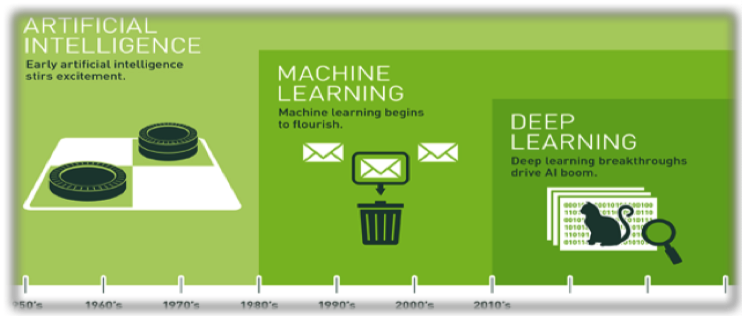
\includegraphics[width=0.8\columnwidth]{Figs/Slide2/ml ai dl.png}		
	\end{center}
\end{alert}

%
\subsubsection{Recent Breakthroughs}
\begin{example}[IBM: \red{Cat-brain}]{s2:5}
	IBM’s \red{Cat-brain} project is a chip like brain (\red{SyNAPSE)} to capture surrounding information in real time. Simulated the cat brain cortex with 147,456 cores and 144TB of memory: basic synaptic circuit for the brain chip.\\
	\red{Current work on $10^9$ artificial neurons and $10^14$ synapses}
\end{example}
\begin{example}[Google: \red{DeepMind}]{s2:6}
	Google’s \red{DeepMind} project, aims at formalizing intelligence to implement in machines and to understand the human brain. Uses \red{deep learning} technologies.\\
	\red{On March 2016, AlphaGo beat the top player in the world (Lee Sedol) in the Go game (Dan 9)}
\end{example}
\begin{example}[IBM: \red{Watson}]{s2:7}
	IBM’s Watson, QA system is used as knowledge repository, to answer virtually any inquiry (in Wikipedia and other knowledge repositories). Uses NLU and ML technologies. Has access to more than $10^9$ pages content.\\
	\red{Won Jeopardy! Contest against top players in the world. Project Intu will equip devices and machines with Watson’s powerful AI tools, hence providing them with cognitive capabilities and make them aware of their environments (ZDNET, Nov. 2016)}
\end{example}
\begin{example}[Amazon, Google and Netflix: Big Data]{s2:8}
	Amazon, Google and Netflix are using Big Data analytics based on Deep Learning to target consumer behavior in various areas including entertainment, shopping and provide adequate recommendations to the user
\end{example}

%
\subsubsection{Origin}
\begin{alert}[Origins of Modern Computing and Machine Learning]{s2:9}
	\begin{center}
		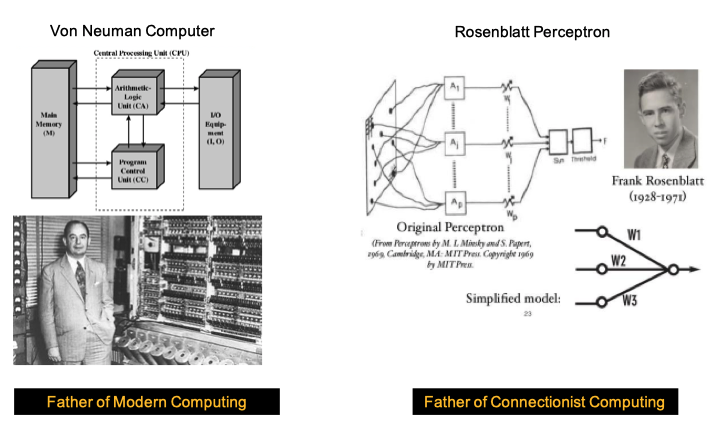
\includegraphics[width=0.8\columnwidth]{Figs/Slide2/origin.png}		
	\end{center}
\end{alert}

%%%
\subsection{Pattern}
\begin{remark}[Notion of a Pattern]{s1:10}
	A pattern is an abstract entity that describes a physical object such as:
	\begin{itemize}
		\item Speech Signal
		\item Handwritten words or digits
		\item Human face
		\item DNA sequence
		\item Weather information
	\end{itemize}
	\begin{center}
		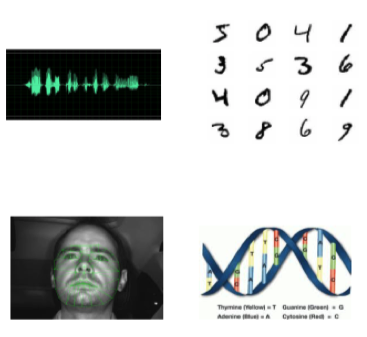
\includegraphics[width=0.6\columnwidth]{Figs/Slide2/pattern.png}		
	\end{center}
\end{remark}
\begin{definition}[Pattern Recognition]{def:pr}
	Pattern recognition (PR) is the study of how machines:
	\begin{itemize}
		\item Observe the environment
		\item Learn to distinguish patterns of interest
		\item Make correct decisions about the
		\item categories of the patterns
	\end{itemize}
	\Gls{PR} involves theory, algorithms, and systems that can assign patterns into categories. \red{More theoretically inclined vs machine learning, which is more practically oriented}.
\end{definition}
\begin{remark}[\Gls{PR} Applications]{s1:11}
	\begin{itemize}
		\item License Plate Recognition
		\item Cancer Detection
		\item Fingerprint Recognition
		\item Autonomous Navigation
	\end{itemize}
	\begin{center}
		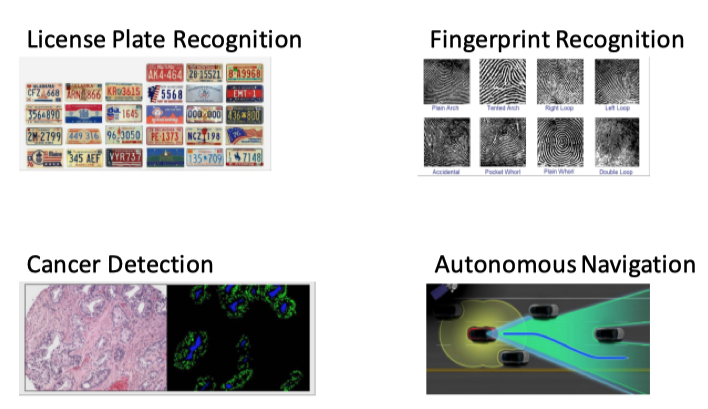
\includegraphics[width=0.6\columnwidth]{Figs/Slide2/app.png}		
	\end{center}
\end{remark}
\begin{algo}[\Gls{PR} Major Approaches]{s1:12}
	\begin{itemize}
		\item Methods for Regression (Continuous Models):
		\vspace{-5pt}
			\begin{itemize}
				\item Least Square
				\item Ridge Regression
				\item The Lasso Approach
			\end{itemize}
		\item Method for Classification (Discrete Modeling):
		\vspace{-5pt}
			\begin{itemize}
				\item Linear and Quadratic Discriminant Analysis
				\item Decision Trees
				\item Rosenblatt's Perceptron
				\item Support Vector Machines
			\end{itemize}
	\end{itemize}
\end{algo}
\begin{remark}[\Gls{PR} Main Challenges]{s1:13}
	\begin{itemize}
		\item Wide variability of the same digits and objects.
		\item How to differentiate between “6” and “0”? it quickly becomes quite complicated to compile a list of heuristics.
		\item If we have more than 5 objects? How can we solve this problem?
		\item Nearly impossible to create handcrafted rules to understand each pixel.
	\end{itemize}
	
	\red{Objective:} design a machine that learns patterns from data!
	\red{Solution:} \Gls{ML}! \Cref{def:ml} \Cref{def:ml:2}
\end{remark}

%%%
\subsection{Machine Learning}
\begin{definition}[Machine Learning]{def:ml:2}
	An area of artificial intelligence (AI) that provides computers with the ability to learn from data while discovering patterns. \red{It doesn't’t follow explicitly programmed instructions.}
\end{definition}
\begin{remark}[]{s1:14}
	It can be applied in situations where it is very challenging or impossible to define heuristic/manual rules e.g., Face detection, Speech recognition, Stock prediction.
\end{remark}
\begin{example}[\Gls{ML}: Leaning to Detect Credit Card Fraud]{s1:15}
	Formally speaking: A ML algorithm improves some measures of performance P when executing some task T through some type of experience E
	\begin{itemize}
		\item Task T: assign category of Fraud/Not Fraud to CC transaction
		\item Performance Measure P: Accuracy of the classifier, i.e, assign higher penalty when Fraud is labeled as Not Fraud
		\item Training Process E: Set of historical credit card training transactions categorized as Fraud or NotFraud
	\end{itemize}
\end{example}
\begin{remark}[\Gls{ML} - Working Mechanism]{s1:16}
	\begin{center}
		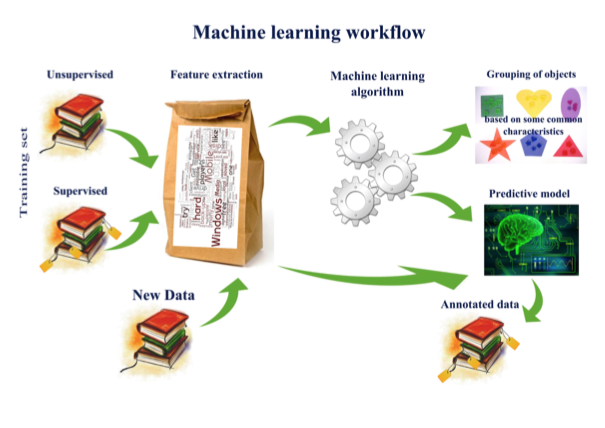
\includegraphics[width=0.8\columnwidth]{Figs/Slide2/ml workflow}
	\end{center}
\end{remark}

\begin{center}
	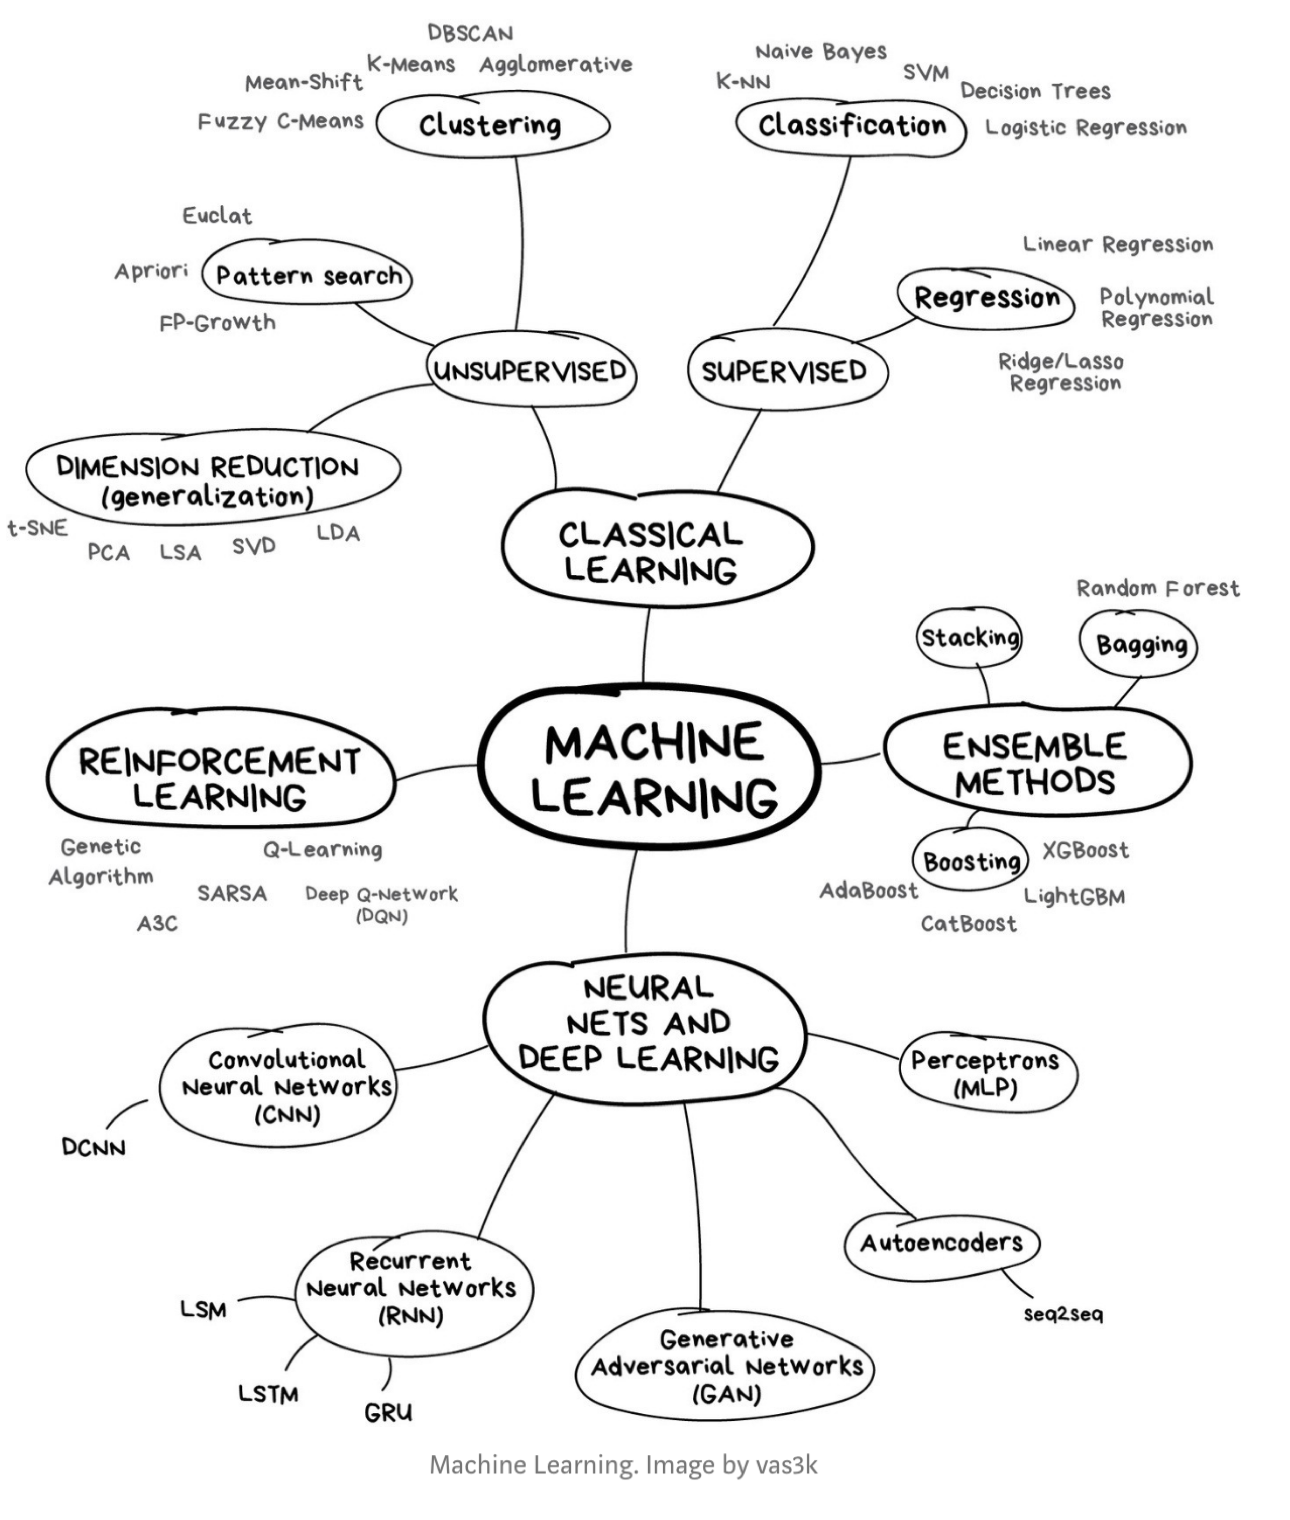
\includegraphics[width=1\columnwidth]{Figs/Slide2/ml tree.png}
\end{center}
	
\begin{remark}[\Gls{ML} - Major Classes]{s1:17}
	\begin{flowchart}
	    % Place nodes
	    \node [block] (ML) {Machine Learning (stochastic or deterministic)};
	    \node [block, below of=ML, node distance=2cm] (US) {Unsupervised};
	    \node [block, left of=US, node distance=5cm] (S) {Supervised};
	    \node [block, right of=US, node distance=5cm] (R) {Reinforcement};
	    \node [block, right of=S, below of=S] (SS) {Semi supervised};
	    \node [tblock, below of=S, node distance=1cm] (TD) {Task Driven};
	    \node [tblock, below of=US, node distance=1cm] (TD) {Data Driven};
	    \node [tblock, below of=R, node distance=1cm] (TD) {Environment Driven};
	    \node [tblock, below of=SS, node distance=4em] (TD) {Combination of supervised and unsupervised learning};
	    % Draw edges
	    \path [line] (ML) -- (S);
	    \path [line] (ML) -- (US);
	    \path [line] (ML) -- (R);
	    \path [line] (S) -- (SS);
	    \path [line] (US) -- (SS);
	\end{flowchart}
\end{remark}


%%%%%%%%%%%%%%%%%%%%%%%%%%%%%%%%%%%%%%%%%%
%%%% Slide 3 - Fundamentals of ANN   %%%%%
%%%%%%%%%%%%%%%%%%%%%%%%%%%%%%%%%%%%%%%%%%
\newpage
\section{Fundamentals of Artificial Neural Network}
%%%% Intro.
\subsection{Introduction}
\begin{overview}[ANNs]{o3:0:0}
	Artificial Neural Networks (ANNs) are the building blocks and the main tools for neuro-computing. they are physical cellular systems, which can acquire, store and utilize experiential knowledge.
	
	ANNs are a set of parallel and distributed computational elements classified according to topologies, learning paradigms and at the way information flows within the network.
	
	ANNs are generally characterized by their:
	\vspace{-5pt}
	\begin{itemize}
		\item Architecture:
			\vspace{-5pt}
			\begin{itemize}
				\item Feedforward
				\item Recurrent
			\end{itemize}
		\item Activation functions:
			\vspace{-5pt}
			\begin{itemize}
				\item Binary
				\item Continuous
			\end{itemize}
		\item Learning Paradigm:
			\vspace{-5pt}
			\begin{itemize}
				\item Supervised
				\item Unsupervised
				\item Hybrid
			\end{itemize}
	\end{itemize}	
\end{overview}


\begin{example}[ANNs Architecture]{ex3:0:1}
	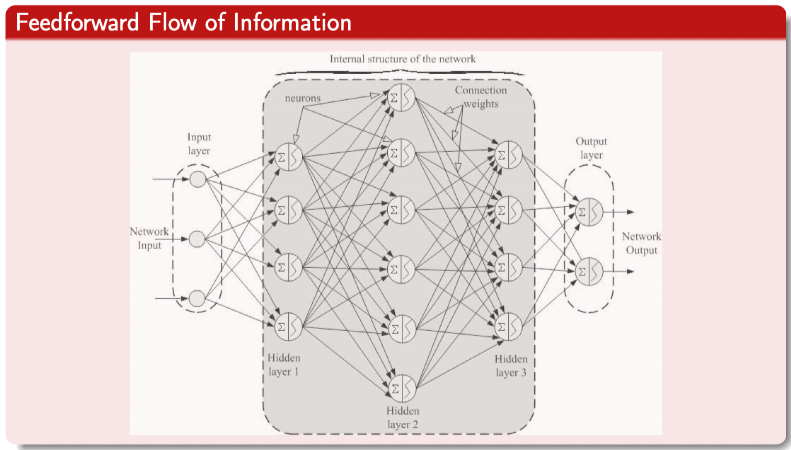
\includegraphics[width=240px]{Figs/Lec4/ff}
	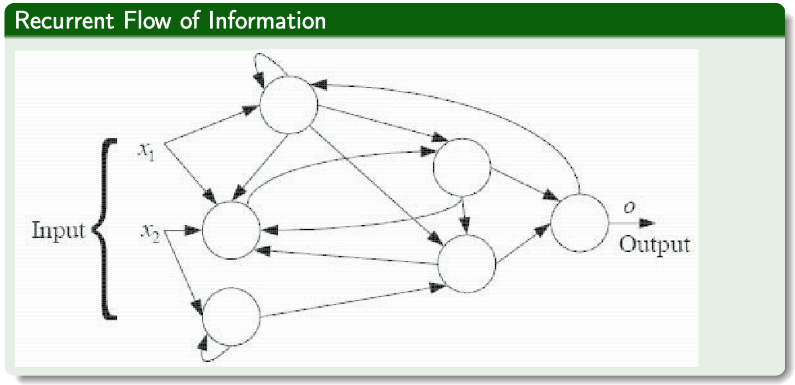
\includegraphics[width=240px]{Figs/Lec4/rr}
\end{example}

\begin{example}[ANNs Activation Functions]{ex3:0:2}
	Binary Activation Functions\\
	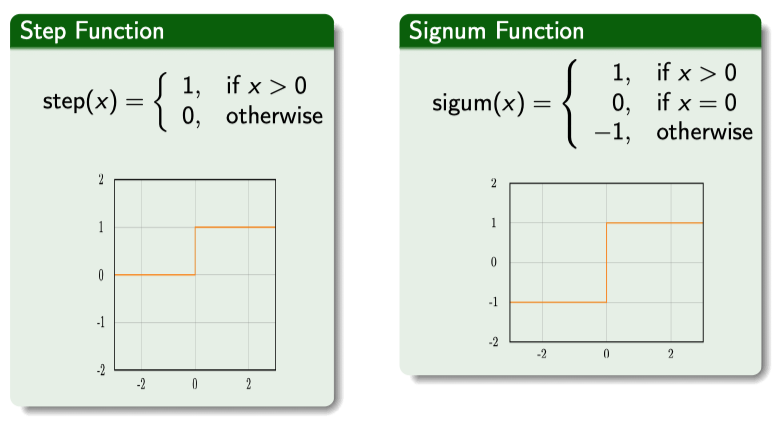
\includegraphics[width=240px]{Figs/Lec4/bin_af}
	
	Differentiable Activation Functions\\
	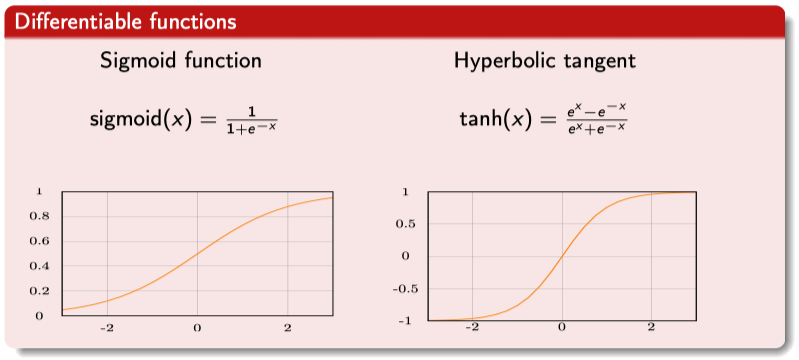
\includegraphics[width=240px]{Figs/Lec4/diff_af}
	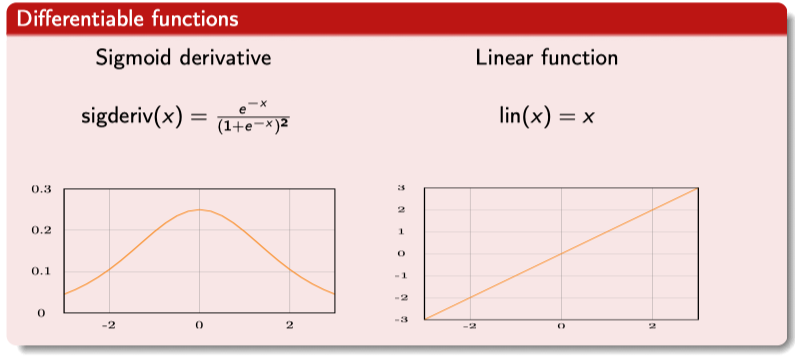
\includegraphics[width=240px]{Figs/Lec4/diff_af2}
\end{example}

\begin{example}[Learning Paradigms]{ex3:0:3}
	\vspace{-5pt}
	\begin{itemize}
		\item Supervised
			\vspace{-5pt}
			\begin{itemize}
				\item Multilayer perceptrons
				\item Radial basis function networks
				\item Modular neural networks 
				\item LVQ (learning vector quantization)
			\end{itemize}
		\item Unsupervised
			\vspace{-5pt}
			\begin{itemize}
				\item Competitive learning networks
				\item Kohonen self-organizing networks
				\item ART (adaptive resonant theory)
			\end{itemize}
		\item Hybrid
			\vspace{-5pt}
			\begin{itemize}
				\item Autoassociative memories (Hopfield networks)
			\end{itemize}
	\end{itemize}
\end{example}

\begin{remark}[Supervised Learning]{r3:0:1}
	\begin{itemize}
		\item Training by example (ex: prior known desired output for each input pattern)
		\item Particularly useful for feedforward network
	\end{itemize}
	
	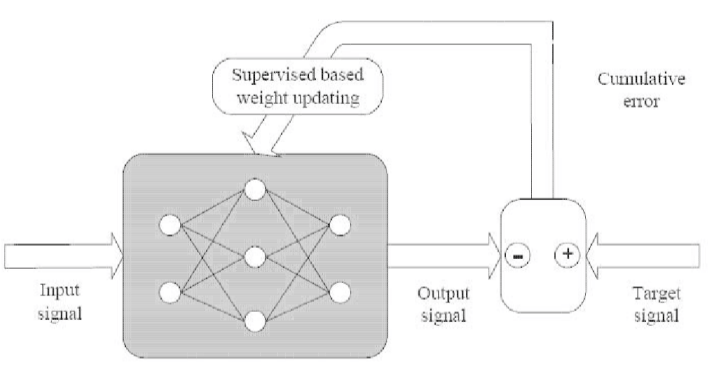
\includegraphics[width=240px]{Figs/Lec4/supervised}
	
	\begin{algo}[Training]{a3:training:supervised}
	\begin{itemize}
		\item Compute error between desired and actual outputs 
		\item Use the error through a learning rule (e.g., gradient descent) to adjust the network’s connection weights 
		\item Repeat steps 1 and 2 for input/output patterns to complete one epoch 
		\item Repeat steps 1 to 3 until maximum number of epochs is reached or an acceptable training error is reached
	\end{itemize}
	\end{algo}
\end{remark}

\begin{remark}[UnSupervised Learning]{r3:0:2}	
	\begin{itemize}
		\item No prior known desired output
		\item In other words, training data composed of input patterns only
		\item Network uses training patterns to discover emerging collective properties and organizes the data into \red{clusters}.
	\end{itemize}
	
	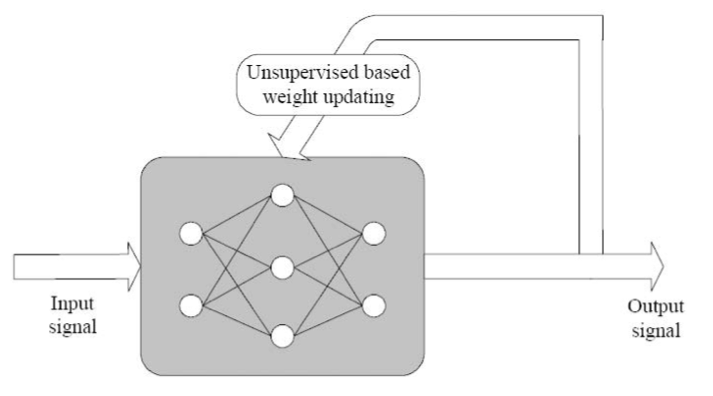
\includegraphics[width=240px]{Figs/Lec4/unsupervised}
	
	\begin{algo}[Training]{a3:training:unsupervised}
	\begin{itemize}
		\item Training data set is presented at the input layer 
		\item Output nodes are evaluated through a specific criterion 
		\item Only weights connected to the winner node are adjusted 
		\item Repeat steps 1 to 3 until maximum number of epochs is reached or the connection weights reach steady state
	\end{itemize}
	\end{algo}
	
	\begin{remark}[Rationale]{r3:0:2:1}
	\begin{itemize}
		\item Competitive learning strengths the connection between the incoming pattern at the input layer and the winning output node.
		\item The weights connected to each output node can be regarded as the center of the cluster associated to that node.
	\end{itemize}
	\end{remark}
\end{remark}

\begin{remark}[Reinforcement Learning]{r3:0:3}
	\begin{itemize}
		\item Reinforcement learning mimics the way humans adjust their behavior when interacting with physical systems (e.g., learning to ride a bike).
		\item Network’s connection weights are adjusted according to a qualitative and not quantitative feedback information as a result of the network’s interaction with the environment or system.
		\item The qualitative feedback signal simply informs the network whether or not the system reacted “well” to the output generated by the network.
	\end{itemize}
	
	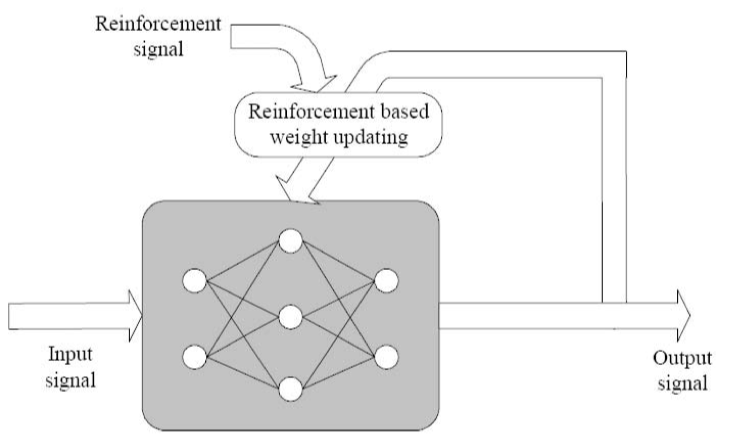
\includegraphics[width=240px]{Figs/Lec4/reinforcement}
	
	\begin{algo}[Training]{a3:training:reinforcement}
	\begin{itemize}
		\item Present training input pattern network
		\item Qualitatively evaluate system’s reaction to network’s calculated output
		\begin{itemize}
			\item If response is \red{“Good”}, the corresponding weights led to that output are \red{strengthened}
			\item If response is \red{“Bad”}, the corresponding weights are \red{weakened}
		\end{itemize}
	\end{itemize}
	\end{algo}
\end{remark}

\begin{remark}[Major Milestones]{r3:0:2}
	\begin{enumerate}
		\item Late 1940’s : McCulloch Pitt Model (by McCulloch and Pitt)
		\item Late 1950’s – early 1960’s : Perceptron (by Roseblatt)
		\item Mid 1960’s : Adaline (by Widrow)
		\item Mid 1970’s : Back Propagation Algorithm - BPL I (by Werbos)
		\item Mid 1980’s : BPL II and Multi Layer Perceptron (by Rumelhart and Hinton)
	\end{enumerate}
\end{remark}


%%%% McCullach-Pitts
\subsection{McCullach-Pitts Model}
\begin{overview}[McCulloch-Pitts Model]{o3:2}
	\begin{itemize}
		\item First serious attempt to model the computing process of the biological neuron
		\item The model is composed of one neuron only
		\item Limited computing capability
		\item No learning capability
	\end{itemize}
\end{overview}


%%%% Perceptron 
\newpage
\subsection{Perceptron}
\red{The first ML algorithm.}
\begin{overview}[Perceptron]{o3:1}
	\begin{itemize}
		\item Uses supervised learning to adjust its weigh ts in response to a comparative signal between the network's actual output and the target output
		\item Mainly designed to classify linearly separable patterns
	\end{itemize}
\end{overview}
\begin{definition}[Linear Separation]{d3:2}
	Patterns are \red{linearly separable} means that there exists a hyperplanar multidimensional decision boundary that classifies the patterns into two classes.
	
	\qquad Linearly separable \qquad \qquad Non-linearly Separable\\
	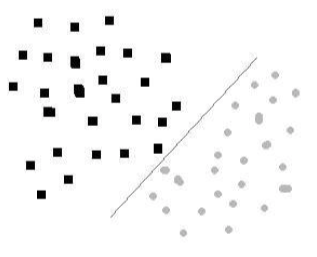
\includegraphics[width=0.3\columnwidth]{Figs/Lec4/linearly_sep}
	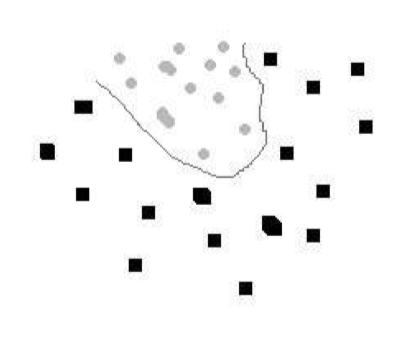
\includegraphics[width=0.3\columnwidth]{Figs/Lec4/non_linearly_sep}
\end{definition}

\begin{remark}[Architecture]{r3:2}
	\begin{itemize}
		\item One neuron (one output)
		\item $l$ input signals: $x_1, \dots, x_l$
		\item Ajustable weights $w_1, \dots, w_l$ and bias $\theta$
		\item Binary activation function (ex: step or hard limiter function)
	\end{itemize}
	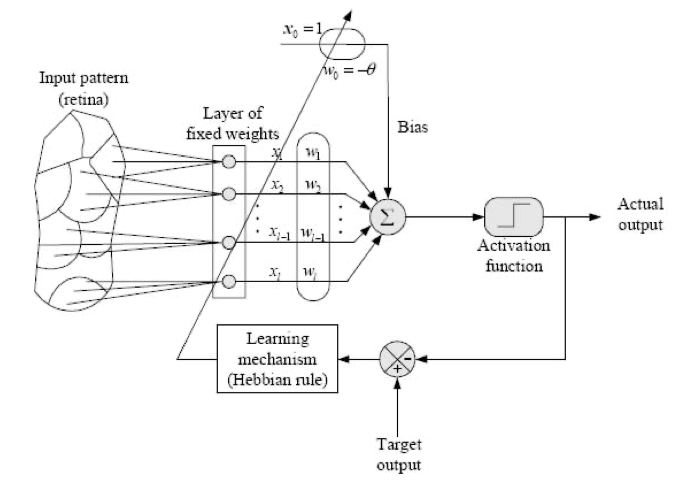
\includegraphics[width=0.6\columnwidth]{Figs/Lec4/architecture}
\end{remark}

\begin{theorem}[Perceptron Convergence Theorem]{t3:1}
	If the training set is \red{linearly separable}, there exists a set of weights for which the training of the Perceptron will \red{converge} in a finite time and the training patterns are correctly classified.
	
	\begin{example}[2D case]{t3:1:e1}
		In the two-dimensional case, the theorem translates into finding the line defined by $w_1 x_1 + w_2 x_2 - \theta = 0$, which adequately classifies the training patterns.

		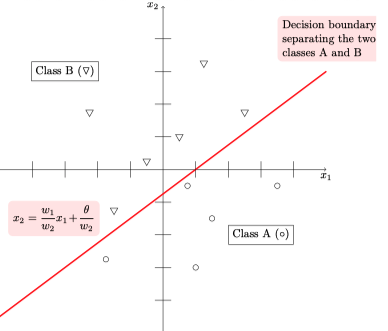
\includegraphics[width=0.4\columnwidth]{Figs/Lec4/perceptron_theorem}
	\end{example}
\end{theorem}

\begin{algo}[Perceptron - Training Algorithm]{a3:perceptron:training}
	\begin{enumerate}
		\item Init weights and thresholds to small random values
		\item Choose an input-output pattern $(x^{(k)}, t^{(k)})$ from the training data
		\item Compute the network's actual output $o^{(k)} = f\left(\sum_{i=1}^{l} w_i x_i^{(k)} - \theta \right)$
		\item Adjust the weights and bias according to the Perceptron learning rule:\\
				$\Delta w_i = \eta [t^{(k)} - o^{(k)}] x_i^{(k)}$, and $\Delta \theta = - \eta [t^{(k)} - o^{(k)}]$, where $\eta \in [0,1]$ is the perceptron's learning rate.
			
				If  f is the \red{signum function}, this becomes equivalent to:
				\begin{equation}
					\Delta w_i = \begin{cases} 2\eta t^{(k)} x_i^{(k)} &, if \, t^{(k)} \neq o^{(k)} \\ 0 & \text{, otherwise}\end{cases} \qquad 
					\Delta \theta_i = \begin{cases} -2\eta t^{(k)} &, if \, t^{(k)} \neq o^{(k)} \\ 0 & \text{, otherwise}\end{cases} 
				\end{equation}
		\item If a whole epoch is complete, then pass to the following step; otherwise go to Step 2.
		\item If the weights and bias reached steady state ($\Delta w_i \approx 0$) through the whole epoch, then stop the learning; otherwise go through one more epoch starting from Step2.
	\end{enumerate}
\end{algo}

\begin{cons}[Perceptron]{c3:1}
	\begin{enumerate}
		\item Cannot separate linearly non-separable patterns
		\item Lack of generalization: once trained, it cannot adapt its weights to a new set of data
	\end{enumerate}
\end{cons}


%%%% Adaline
\newpage
\subsection{Adaline (Adaptive Linear Neuron)}
\begin{overview}[Adaline]{o3:2}
	\begin{itemize}
		\item More versatile than the Perceoptron in terms of generalization
		\item More powerful in terms of weight adaptation
		\item An Adaline is composed of a linear combiner, a binary activation function (hard limiter), and adaptive weights
	\end{itemize}
	
	\begin{note}[Graphical Illustration]{pink}{n3:2}
		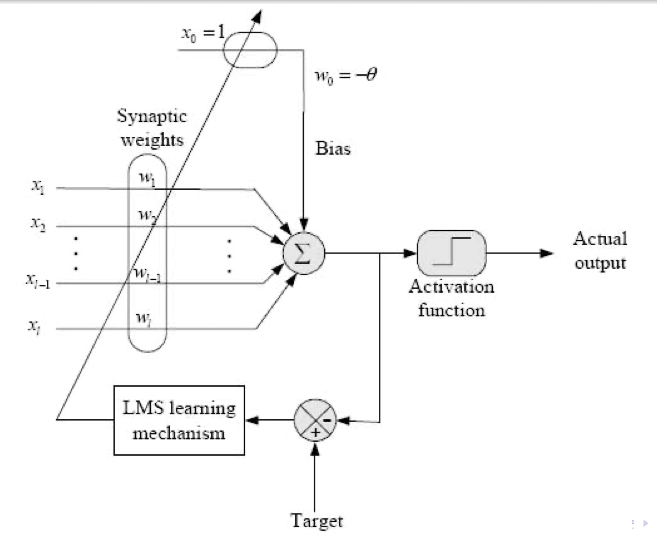
\includegraphics[width=0.5\columnwidth]{Figs/Lec4/adaline}
	\end{note}
\end{overview}

\begin{remark}[Learning in an Adaline]{r3:4}
	\begin{itemize}
		\item Adaline adjusts its weights according to the least mean squared (LMS) algorithm (also known as the \red{Widrow-Hoff learning rule}) through gradient descent optimization.
		\begin{alert}[LMS]{alert:3:1}
				\red{Widrow-Hoff learning rule} $\equiv$ LMS (Least Mean Square)
		\end{alert}
		\item At every iteration, the weights are adjusted by an amount of proportional to the gradient of the cumulative error of the network \red{$E(w) \Rightarrow \Delta w = - \eta \nabla_w E(w)$}
		\item The network's total error $E_c(w)$ for all patterns $(x^{(k)}, t^{(k)}), k = 1, 2, \dots, n$. This is the cumulative error involving all training data and ait is between the desired response $t^{(k)}$ and the linear combiner's output $(\sum_i w_i x_i^{(k)} - \theta)$. It is expressed as:
			\begin{equation}
				E_c(w) = (1/2) \sum_k \left[ t^{(k)} - (\sum_i w_i x_i^{(k)} - \theta)\right]^2
			\end{equation}
		\item All patterns have to be represented here and the cumulative error has to be computed. This is referred as \red{batch training} and it is time consuming
		\item Instead we compute individual errors based on the presented pattern (k) and keep updating the weights each time a pattern in the epoch is presented. This is known as \red{on-line training}.
			\begin{equation}
				E^k(w) = (1/2) \left[ t^{(k)} - (\sum_i w_i x_i^{(k)} - \theta)\right]^2
			\end{equation}
		\item Hence, individual weights are updated using \red{$\Delta w =  - \eta \nabla_w E^k(w)$} as:
			\begin{equation}
				\Delta w_i = \eta \left( t^{(k)} - \sum_i w_i x_i^{(k)} \right) x_i^{(k)}
			\end{equation}
	\end{itemize}
\end{remark}

\begin{algo}[Adaline - Training Algorithm]{a3:adaline:training}
	\begin{enumerate}
		\item Init weights and thresholds to small random values
		\item Choose an input-output pattern $(x^{(k)}, t^{(k)})$ from the training data
		\item Compute the network's actual output $r^{(k)} = \sum_{i=1} w_i x_i^{(k)} - \theta $
		\item Adjust the weights and bias according to the \red{LMS} rule:\\
				$\Delta w_i = \eta \left( t^{(k)} - \sum_{i} w_i x_i^{(k)} \right) x_i^{(k)}$, where $\eta \in [0,1]$ is the perceptron's learning rate.
		\item If a whole epoch is complete, then pass to the following step; otherwise go to Step 2.
		\item If the weights and bias reached steady state ($\Delta w_i \approx 0$) through the whole epoch, then stop the learning; otherwise go through one more epoch starting from Step2.
	\end{enumerate}
\end{algo}

\begin{pros}[LMS Algorithm]{pro3:1}
	\begin{itemize}
		\item Easy to implement
		\item Suitable for generalization, which is a missing feature in the Perceptron
	\end{itemize}
\end{pros}
\begin{cons}[Adaline]{con3:2}
The adaline, while having attractive training capabilities, suffers also (similarly to the perceptron) from the inability to train patterns belonging to nonlinearly separable spaces.
\end{cons}

\begin{remark}[Madaline]{r3:2:1}
	Researchers have tried to circumvent this difficulty by setting cascade layers of adaline units.

	When first proposed, this seemingly attractive idea did not lead to much improvement due to the lack of an existing learning algorithm capable of adequately updating the synaptic weights of a cascade architecture of perceptrons.
	
	Other researchers were able to solve the nonlinear separability problem by combining in parallel a number of adaline units called a madaline.

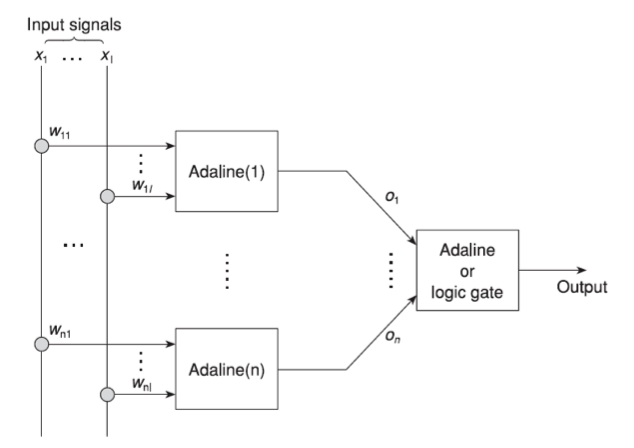
\includegraphics[width=0.5\columnwidth]{Figs/Lec4/madaline}

\begin{example}[Madaline]{ex3:madaline}
	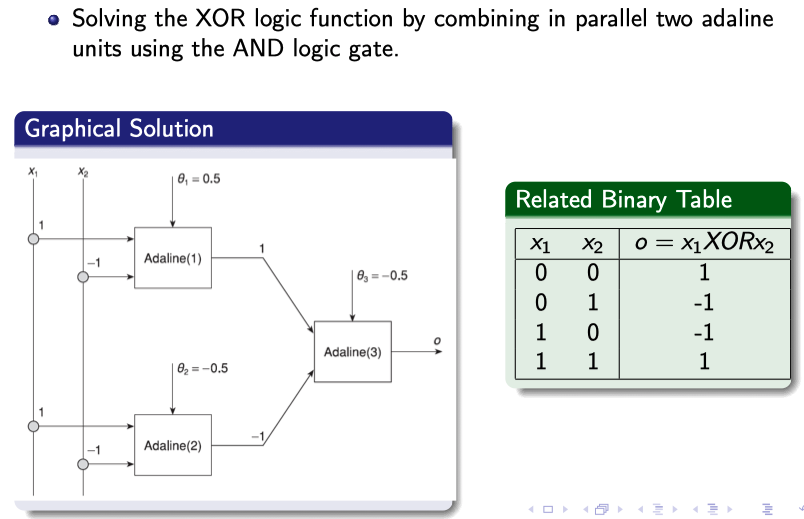
\includegraphics[width=0.8\columnwidth]{Figs/Lec4/madaline_ex}	
\end{example}
\end{remark}

\begin{remark}[Madaline]{r3:madline}
	\begin{itemize}
		\item Despite the successful implementation of the adaline and the madaline units in a number of applications, many researchers conjectured that to have successful connectionist computational tools, neural models should involve a topology with a number of cascaded layers.
		\item Schematics of the madaline implementation of the backpropagation learning algorithm to neural network models composed of multiplelayers of perceptrons.
	\end{itemize}
\end{remark}
%%%


\newpage
%%%%%%%%%%%%%%%%%%%%%%%%%%%%%%%%%%%%%%%%%%%%%%%%%%%%%%%%%%%%%%%%%%%%%%%%%%%%%%%%
%% ************************************************************************** %%
%% *                               Chapter 03                               * %%
%% ************************************************************************** %%
%%%%%%%%%%%%%%%%%%%%%%%%%%%%%%%%%%%%%%%%%%%%%%%%%%%%%%%%%%%%%%%%%%%%%%%%%%%%%%%%
\chapter{Classes of \Gls{ML} models}
%%%%%%%%%%%%%%%%%%%%%%%%%%%%%%%%%%%%%%%%%%%%%%%%%%%%%%
%%%% Slide 4 - Major Classes of Neural Network   %%%%%
%%%%%%%%%%%%%%%%%%%%%%%%%%%%%%%%%%%%%%%%%%%%%%%%%%%%%%
\section{Major Classes of Neural Network}
%%%% Intro.
\subsection{MLPs: Multi-Layer Perceptrons}
\begin{note}[Background]{pink}{n4:mlp}
\begin{itemize}
	\item The perceptron lacks the important capability of recognizing patterns belonging to non-separable linear spaces
	\item The madaline (\Cref{r3:madline}) is restricted in dealing with complex functional mappings and multi-class pattern recognition problems
	\item The multilayer architecture first proposed in the late 60s
	\item MLP re-emperhed as a solid connectionist model to solve a wide range of complex problems in the mid-80s
	\item This occurred following the reformulation of a powerful learning algorithm commonly called the \red{Back Propagation Learning} (\Gls{BPL})
	\item It was later implemented to the multilayer perceptron topology with a great deal of success
\end{itemize}

	\textbf{Schematic Representation of MLP Network}\\
	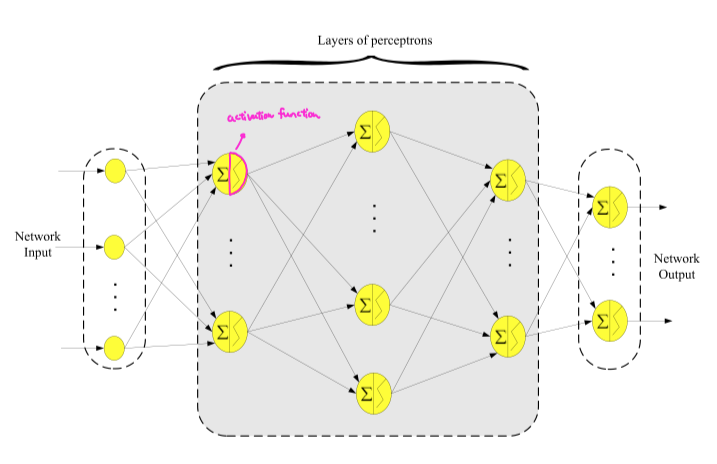
\includegraphics[width=340px]{Figs/Lec5/MLP_schematics}
\end{note}

\clearpage
\begin{overview}[\Gls{BPL}]{o4:bpl}
	\begin{itemize}
		\item The \Gls{BPL} is based on the \red{gradient descent technique} involving the \red{minimization of the network cumulative error}.
			\begin{equation}
				E(k) = \sum_{i=1}^q \left[ t_i(k) - o_i(k) \right]^2
			\end{equation}
			\begin{eqconditions}
				i & i-th neuron of the output layer \\
				q & number of output neurons
			\end{eqconditions}
		\item It is designed to \red{update the weights} in the \red{direction of the gradient descent} of the cumulative error
	\end{itemize}

	\begin{algo}[Two Stage Algorithm]{}
	\begin{enumerate}
		\item Patterns are presented to the network
		\item A feedback signal is then propagated backward with the main task of updating the weights of the layers connections according to the \Gls{BPL}.
	\end{enumerate}
	\end{algo}
	
	\textbf{Schematic Representation of \Gls{BPL} Network} illustrating the notion of \red{error back-propagation}.\\
	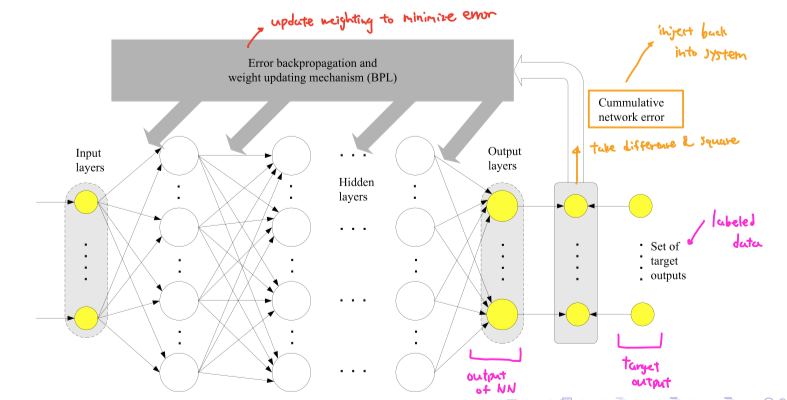
\includegraphics[width=340px]{Figs/Lec5/BPL_schematics.png}
	
	\begin{remark}[Objective Function]{r4:bpl:objfunc}
		- Using the \red{sigmoid function} as the activation function for all the neurons of the network, we defined $E_c$ as 
		\begin{equation}
			E_c = \sum_{k=1}^n E(k) = \frac{1}{2} \sum_{k=1}^n \sum_{i=1}^q [t_i (k) - o_i (k)]^2
		\end{equation}
		
		- the formulation of the \red{optimization problem} can now be stated as \red{finding the set of the network weights} that minimizes $E_c$ or $E(k)$

		\begin{equation}
			\textbf{Offline Training: } \quad \min_w E_c = \min_w  \frac{1}{2} \sum_{k=1}^n \sum_{i=1}^q [t_i (k) - o_i (k)]^2
		\end{equation}
		
		\begin{equation}
			\textbf{Online Training: } \quad \min_w E(k) = \min_w  \frac{1}{2} \sum_{i=1}^q [t_i (k) - o_i (k)]^2
		\end{equation}
	\end{remark}
\end{overview}

\subsubsection{\Gls{BPL}: On-line Training}
\begin{remark}[\Gls{BPL}: On-line Training]{r4:online-bpl}
	\textbf{Objective Function: } 
	\begin{equation}
		\quad \min_w E(k) = \min_w  \frac{1}{2} \sum_{i=1}^q [t_i (k) - o_i (k)]^2
	\end{equation}
	
	\begin{remark}[Updating Rule for Connection Weights]{r4:conn_weight}
		\begin{equation}
			\Delta w^{(l)} = - \eta \frac{\partial E(k)}{\partial w^{(l)}}
		\end{equation}

		\begin{eqconditions}
			l 				& (l-th) layer \\
			\eta 			& learning rate \\
			\Delta w_{ij}^l & the weight update for the connection linking the node $j$ of layer $(l-1)$ to node $i$ located at layer $l$ \\
			o_j^{l-1} 		& the output of the neuron $j$ at layer $l-1$, the one located just before layer $l$ \\
			tot_i^l 		& the sum of all signals reaching node $i$ at hidden layer $l$ coming from previous layer $l-1$
		\end{eqconditions}
	\end{remark}
	
	\begin{example}[Illustration of interconnection between layers of \Gls{MLP}]{ex4}
		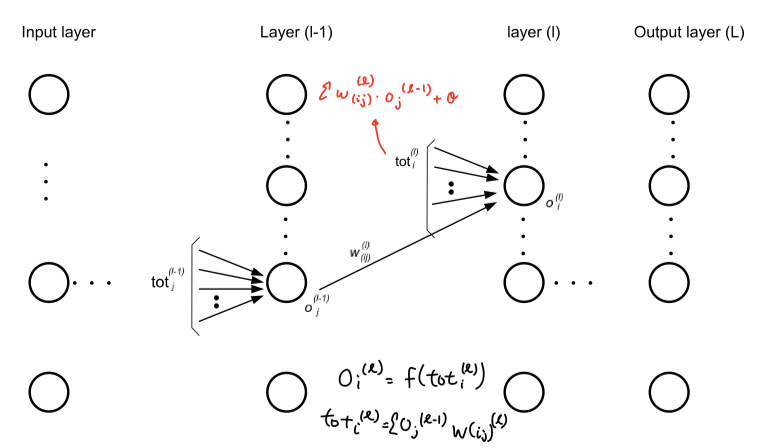
\includegraphics[width=340px]{Figs/Lec5/BPL_illustration}
	\end{example}
	
	\begin{remark}[Interconnection Weights Updating Rules]{r4:inter-rules}
		\begin{itemize}
			\item $\Delta w^{(l)} = \Delta w_{ij}^{(l)} = - \eta \frac{\partial E(k)}{\partial w^{(l)}} = - \eta [\frac{\partial E(k)}{\partial o_i^{(l)}}][\frac{\partial o_i^{(l)}}{\partial tot_i^{(l)}}][\frac{\partial tot_i^{(l)}}{\partial w_{ij}^{(l)}}]$
			\item For the case where the layer $(l)$ is the output layer $(L)$:\\ 
				$\Delta w_{ij}^{(L)} = \eta [t_i - o_i^{(L)}][f'(tot)_i ^{(L)}] o_j^{(L-1)} ; \quad f'(tot)_i^{(l)} = \frac{\partial \, f(tot_i^{(l)})}{\partial \, tot_i^{(l)}}$
			\item By denoting $\delta_i^{(L)} = [t_i - o_i^{(L)}][f'(tot)_i ^{(L)}]$ as being the \red{error signal} of the i-th node of the output layer, the weight update at layer (L) is as follows: $\Delta w_{ij}^{(L)} = \eta \delta_i^{(L)} o_j^{(L-1)}$
			\item In the case where $f$ is the sigmoid function $f(x) = \frac{1}{1 + e^{-x}}$, the error signal becomes expressed as: \\ $\delta_i^{(L)} = [(t_i - o_i^{(L)})o_i^{(L)}(1-o_i^{(L)})]$
			\item Propagating the error backward now, and for the case where $(l)$ represents a hidden layer $(l < L)$, the expression of $\Delta w_{ij}^{(L)}$ becomes given by: $\Delta w_{ij}^{(l)} = \eta \delta_i^{(l)} o_j^{(l-1)}$, where $\delta_i^{(L)} = f' (tot)_i^{(l)} \sum_{p=1}^{n_{l+1}} \delta_p^{(l+1)} w_{pi}^{(l+1)}$
			\item Again, when $f$ is taken as the sigmoid function, $\delta_i^{(l)}$ becomes expressed as: \\
				$\delta_i^{(l)} = o_i^{(l)} (1-o_i^{(l)}) \sum_{p=1}^{n_{l+1}} \delta_p^{l+1} w_{pi}^{l+1}$
		\end{itemize}
	\end{remark}
\end{remark}

\begin{alert}[...]{a4:end}
	Rest Slides are open to read: Off-line BPL for MLP
\end{alert}

\newpage
%%%%%%%%%%%%%%%%%%%%%%%%%%%%%%%%%%%%%%%%%%%%%%%%%%%%%%%%%%%%%%
%%%% Slide 6 - Variance, Bias, Underfiting, and Overfiting %%%%%
%%%%%%%%%%%%%%%%%%%%%%%%%%%%%%%%%%%%%%%%%%%%%%%%%%%%%%%%%%%%%%
\section{Variance, Bias, Underfiting, and Overfiting}
%%%% ML Models
\subsection{Machines Learning Model}
\begin{overview}[Machine Learning - Main Idea]{o6:ml}
		The idea is to extract the best model form a set of collected data, which could predict future occurences (whether for classification, which involves discrete output or regression which involves continuous output).
		
		The data collected is usually corrupted with noise or is recorded wrongly.
\end{overview}

\begin{remark}[Types of \Gls{ML} Models]{r6:types_ml}
	\begin{definition}[Classification]{d6:classification}
		Given samples from two (or more classes), find a boundary (linear or non-linear) that separates them with minimum incorrect classifications.
	\end{definition}	
	\begin{definition}[Regression]{d6:regression}
		Find the continuous relationship between two variables $x_1$ and $x_2$ using only samples and no prior knowledge of their distribution.
	\end{definition}
\end{remark}

\begin{example}[Learning Model for Classification]{ex6:class}
	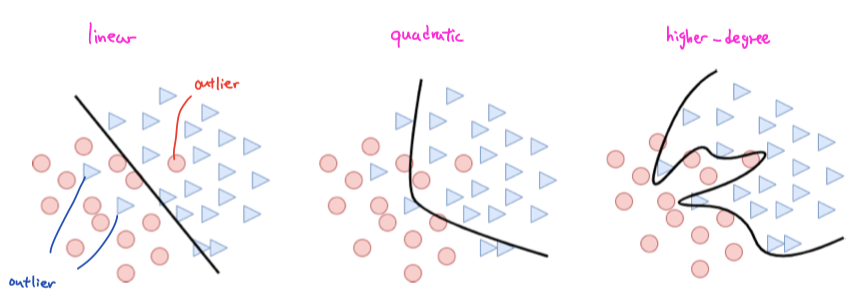
\includegraphics[width=350px]{Figs/Lec6/class_lm.png}
	
	Classification of two classes with a polynomial function having different degrees of freedom. 
\end{example}

\begin{example}[Learning Model for Regression]{ex6:reg}
	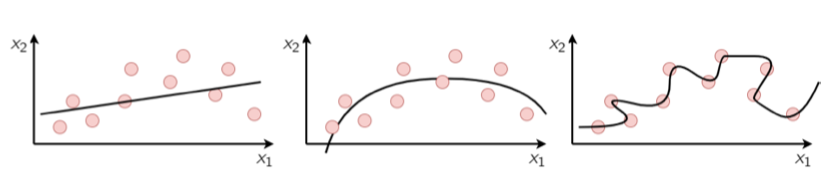
\includegraphics[width=350px]{Figs/Lec6/reg_lm.png}
	
	Regression of data with a polynomial function having different degrees of freedom.
\end{example}

\clearpage
\begin{example}[Classification]{ex6:class-ex}
	We want to teach a baby (model) the difference between tomato and cucumber. We show it several tomato and say these are tomatoes. We do the same for cucumbers. The baby learns to classify tomatoes from cucumbers. The baby can find out whether a new unseen vegetable is a tomato or cucumber. The out put of classification (whether is tomato or cucumber) is \red{discrete}.
\end{example}

\begin{example}[Regression]{ex6:reg-ex}
	 We want to make an artificial leg for people without leg s. Using the Electromyography (EMG) signals in a health y leg , we collect which signals result in which degrees of knee. The learned artificial leg , when is installed, can estimate the knee degree for new unlearned EMG signals. The output of regression (the knee degree) is \red{continuous}.
\end{example}

%%%% Data
\subsection{Training, Validation, and Test Data}
\begin{remark}[Training, Validation, and Test Data]{r6:data}
	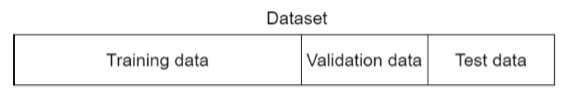
\includegraphics[width=350px]{Figs/Lec6/dataset}
	
	Dataset can be divided into disjoint training, validation, and test sets:
	\begin{definition}[Training Dataset]{def6:data-train}
		used for \red{teaching} the model
	\end{definition}
	\begin{definition}[Validation Dataset]{def6:data-valid}
 		used for either \red{selection of hyper-parameters} or \red{checking overfitting} (introduced later) during the training phase.
	\end{definition}
	\begin{definition}[Test Dataset]{def6:data-test}
		used for testing the trained model (to see how good its performance is). This is never seen by the model during training and cannot affect the weights in any way.
	\end{definition}
\end{remark}

%%%% Bias and Var
\subsection{Bias and Variance}
\begin{remark}[Evaluating a Model]{r6:eval}
	The error in predictions is defined as the difference between the predicted values and the actual (ground-truth) values. Two major metrics in direct correlation with the predition error are then used to assess the goodness of a model:
	\begin{itemize}
		\item Variance
		\item Bias
	\end{itemize}
	
	\begin{definition}[Expected Value]{def:exp-val}
		What we expect from a random variable to be on \red{average} (a.k.a. mean $\mu$).
			\begin{equation}
				\mathbb{E}(\hat{X}) := \sum_{x_i \in \hat{X}} x_i {\mathbb{P}(x_i)}
			\end{equation}
	\end{definition}
	
	\begin{definition}[Variance]{def:var}
		How \red{spread} the values of a random variable are.
			\begin{equation}
				\mathbb{V}ar (\hat{X}) := \mathbb{E}\left((\hat{X} - \mathbb{E}(\hat{X}))^2 \right) = \mathbb{E}(\hat{X}^2) - (\mathbb{E}(\hat{X}))^2
			\end{equation}
	\end{definition}
	
	\begin{definition}[Bias]{def:bias}
		How different the expected value of a random variable is from its actual value
			\begin{equation}
				\mathbb{B}ias(\hat{X}):= \mathbb{E}(\hat{X}) - X
			\end{equation}
	\end{definition}
\end{remark}

\begin{example}[Variance and Bias - Dart Illustration]{ex6:dart}
	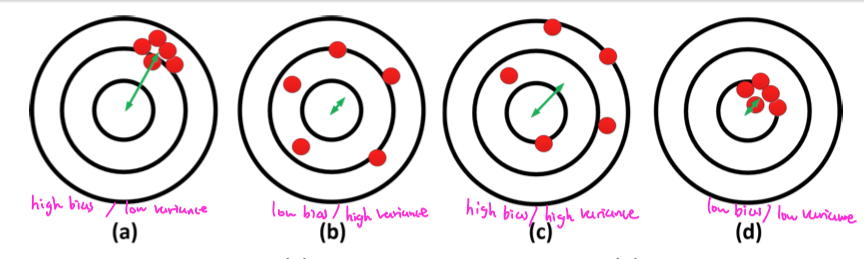
\includegraphics[width=350px]{Figs/Lec6/var}
	
	The dart example for (a) high bias and low variance, (b) low bias and high variance, (c) high bias and high variance, and (d) low bias and low variance. 

	The worst and best cases are (c) and (d), respectively. 
	
	The center of the circles is the true values of variable
	
	The green double arrow denotes the distance to the center of the average of the predicted values.
\end{example}

\begin{remark}[Variance in \Gls{ML}]{r6:var-in-ml}
	A variance is defined as the amount that the estimate of the \red{target boundary (classification)} or \blue{target function (regressor)} will change if different data points were used.
	
	\begin{itemize}
		\item \textbf{High Variance}: \red{Significant} changes
		\item \textbf{Low Variance}: \blue{Minor} changes
	\end{itemize}
\end{remark}

\begin{remark}[Variance in Learning Models]{r6:var-in-lm}
	Usually, \red{complex machine learning algorithms (nonlinear)} have \red{HIGH} variance.
	
	\begin{center}
		\begin{tabular}{| c || c |} 
			\hline
		 	\blue{Low Variance} & \red{High Variance} \\ 
		 	\hline\hline
		 	Linear Regression (LRG) 			& Polynomial RG and Decision Trees		\\
		 	Linear Discriminant Analysis 	& Support Vector Machines (\Gls{SVM})	\\
		 	Logistic Regression 				& Multi-layer Neural Networks			\\
		 	Naive Bayes						& K-Nearest Neighbours					\\
			\hline\hline
		\end{tabular}
	\end{center}
\end{remark}

\begin{remark}[Bias in \Gls{ML}]{r6:bias-in-ml}
	A bias is the amount that the estimate of the \red{target boundary (classification)} or \blue{target function (regressor)} classifies or regresses training data points correctly.
	
	(How distinct/far the data from the estimate)
	
	\begin{itemize}
		\item \textbf{High Bias}: \red{Very bad} performance of the model on the training data
		\item \textbf{Low Bias}: \blue{Good and acceptable} performance of the model on the training data
	\end{itemize}
	
	\begin{alert}[]{a6:bias-in-ml}
		Both high and low biased models may perform poorly on the testing data; hence, a \blue{medium bias} is usually desired.
	\end{alert}

	\begin{example}[Bias in Classification]{ex6:bias-in-ml-class}
		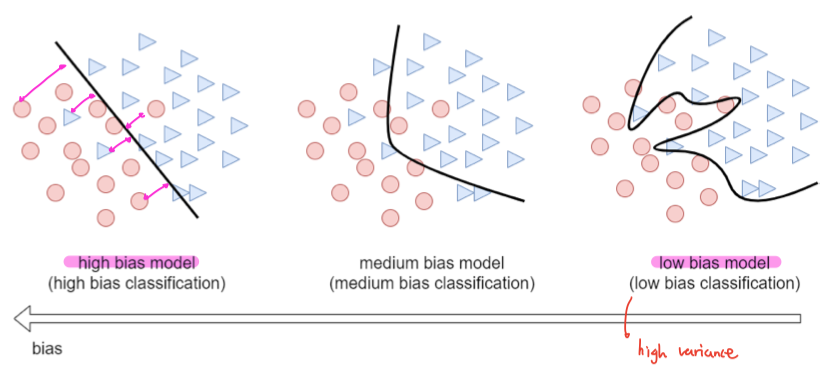
\includegraphics[width=360px]{Figs/Lec6/bias-class}
	\end{example}

	\begin{example}[Bias in Regression]{ex6:bias-in-ml-reg}
		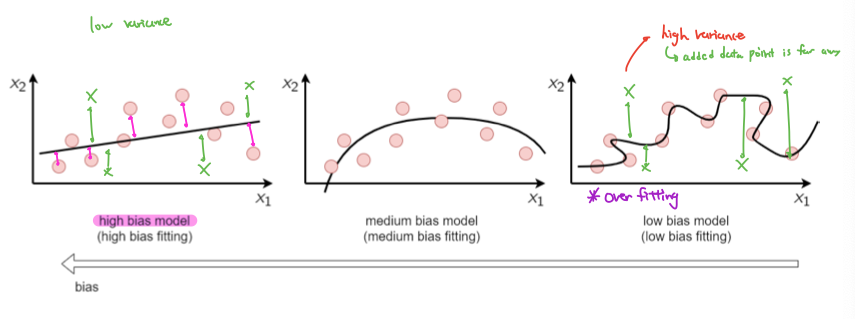
\includegraphics[width=360px]{Figs/Lec6/bias-reg}
	\end{example}	
\end{remark}

\clearpage
%%%% Fitting & Generalization
\subsubsection{Underfitting, Overfitting, and Generalization}
\begin{remark}[Overfitting]{r6:overfit}
	An intuitive example for overfitting is as follows. Assume the model is a baby to whom we want to teach what a coffee cup is:
	
	\begin{itemize}
		\item \textbf{Under-fit}: "a cup is like a glass" $\Rightarrow$ \red{confuses} glass with cup
		\item \textbf{Good-fit}: "a coffee cup usually has a cap, too." $\Rightarrow$ \blue{generalize} tp new unseen coffee cups
		\item \textbf{Over-fit}: "Coffee cup has the shape of a leaf on it." $\Rightarrow$ only able to recognize Tim Hortons cups and not Starbucks cups. $\Rightarrow$ The baby(model) \red{memorizes} rather than learns.
	\end{itemize}
	
	\begin{example}[Overfitting in Classification]{ex6:ovf-in-ml-class}
		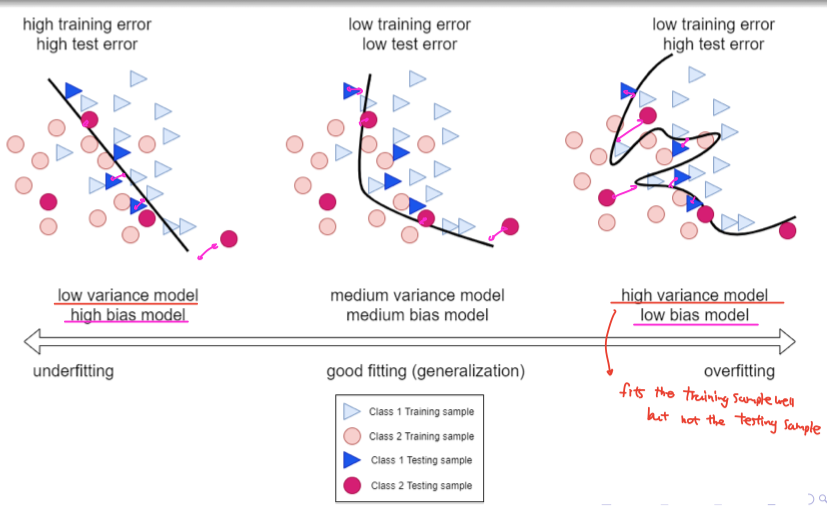
\includegraphics[width=400px]{Figs/Lec6/ovf-class}
	\end{example}

	\begin{example}[Overfitting in Regression]{ex6:ovf-in-ml-reg}
		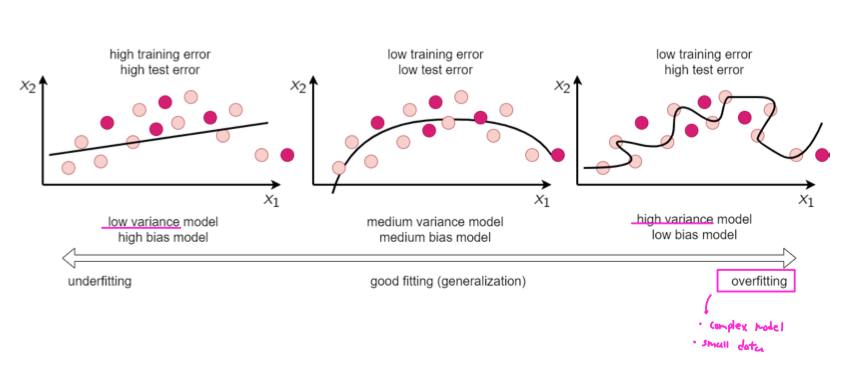
\includegraphics[width=400px]{Figs/Lec6/ovf-reg}
	\end{example}	
\end{remark}

\clearpage
\begin{remark}[Diagram of Error in Training]{r6:diag-error}
	 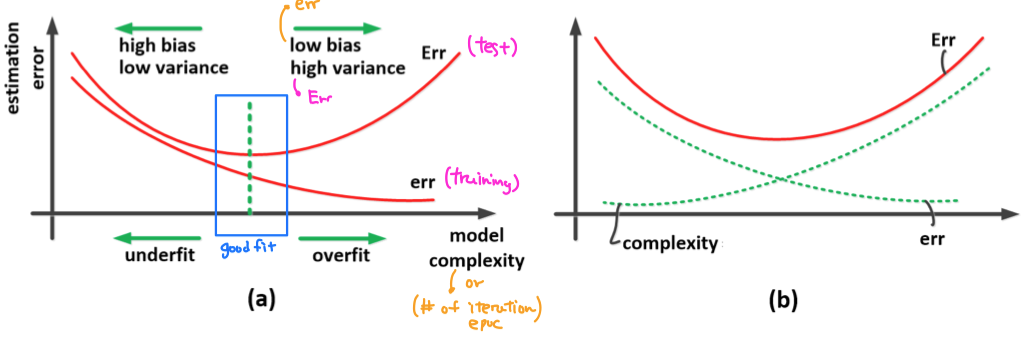
\includegraphics[width=450px]{Figs/Lec6/diag-err}
	 
	 (a) \red{Training error (err)} v.s. \blue{test/validation err (Err)}
	 
	 (b) The more complex the model gets, if it is not trained by sufficient data, we will have overfitting.
\end{remark}

\begin{remark}[Underfitting vs. Overfitting]{r6:ovf-vs-unf}
	\begin{definition}[Underfitting]{def6:underfitting}
		Model fails to capture the underlying trend of the data and performs poorly on both training and testing sets (\red{high bias and low variance}), Caused by:
		
		\begin{itemize}
			\item Model too simple (linear or 1st order polynomial), Low Complexity	
			\item Training data is not enough to capture the complete behaviour of the process
		\end{itemize}
	\end{definition}
	\begin{definition}[Overfitting]{def6:overfitting}
		Model corresponds too closely to training dataset, capturing the noise and inaccuracies, therefore performing poorly on the testing set (no generalization - \red{low bias and high variance}).
		\begin{itemize}
			\item Model too complex and rigidly tied to training data (inflexible)
			\item Training data not containing enough variety to describe the entire population
			\item Too many training iterations (in iterative training algorithms)
		\end{itemize}
	\end{definition}	
\end{remark}

\begin{example}[Trade-off Design: Bias vs. Variance (1)]{ex6:trade-off-design}
	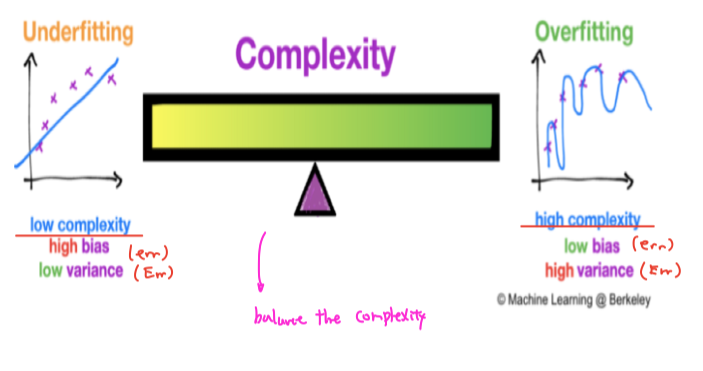
\includegraphics[width=280px]{Figs/Lec6/gen-1.png}
\end{example}

\begin{example}[Trade-off Design: Bias vs. Variance (2)]{ex6:trade-off-design2}
	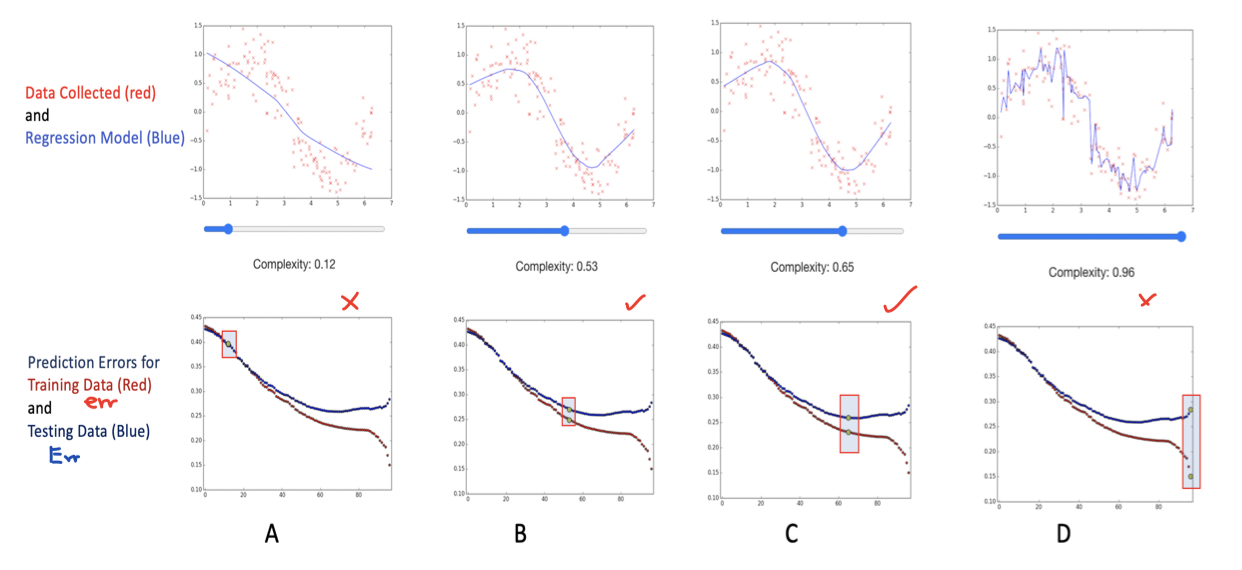
\includegraphics[width=450px]{Figs/Lec6/gen-2.png}
	
	\red{Training} and \blue{Testing} erros vs. complexity levels of proposed models
	
	\begin{itemize}
		\item A: Simple (High Bias) and prone to Underfitting
		\item D: Complex (High Variance) and prone to overfitting
		\item \blue{B and C}: Better Genralizers of the data (medium bias and medium variance)
	\end{itemize}
\end{example}

\begin{example}[Trade-off Design: Bias vs. Variance (3)]{ex6:trade-off-design3}
	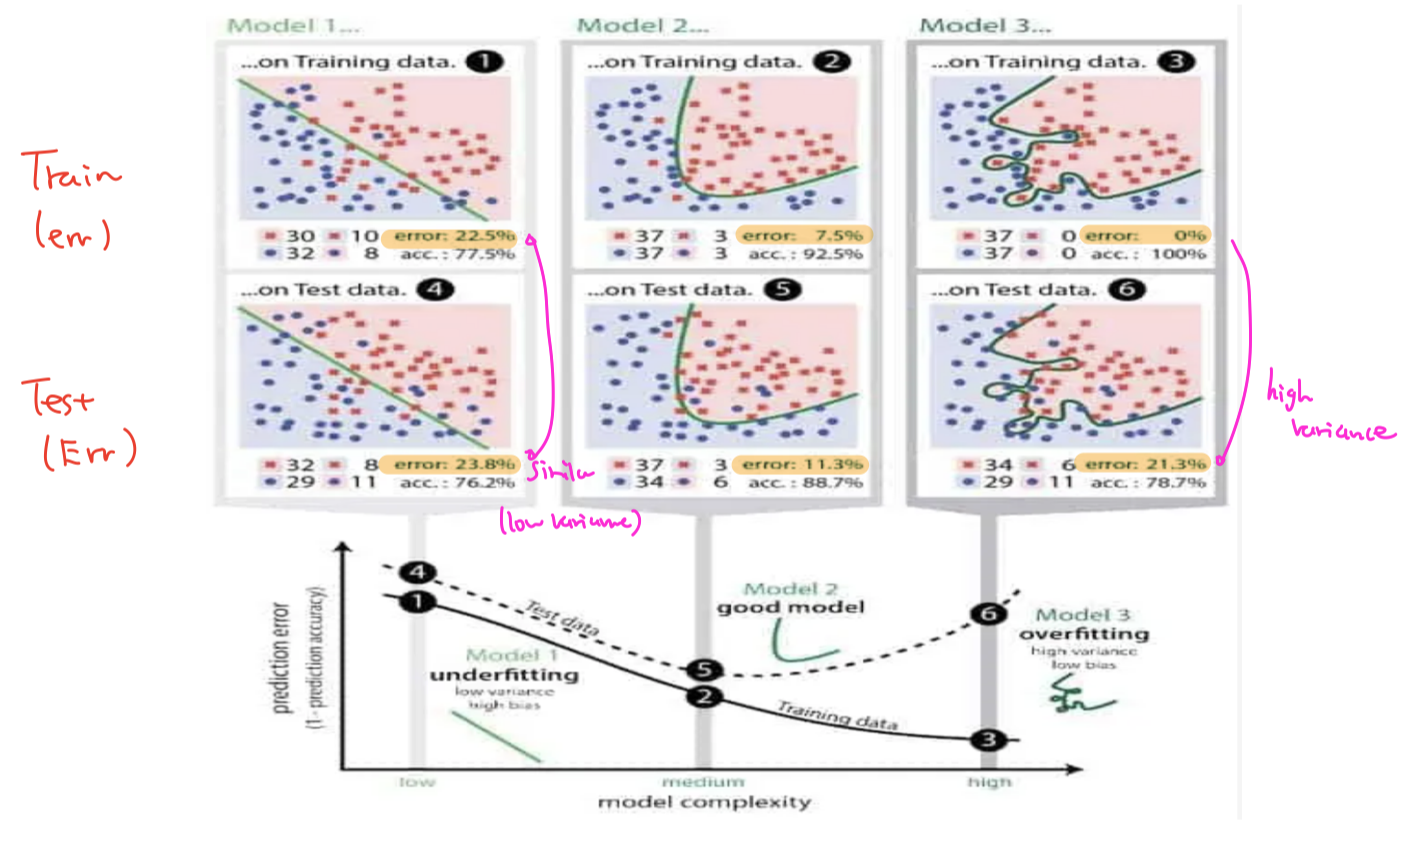
\includegraphics[width=450px]{Figs/Lec6/gen-3.png}
\end{example}


\clearpage
%%%% How to avoid bad fitting
\subsubsection{How to avoid Under-fitting and Over-fitting}
\begin{overview}[Dealing with Under-fitting and Over-fitting]{o6:deal-with-fitting}
	The nature of the algorithm dictates whether the model is high variance or high bias.
	
	\begin{remark}[Solving for Under-fitting]{r6:solv-under}
		\begin{enumerate}
			\item Add more training data to the system to capture complex behavior of the model
			\item Make the model more complex (adding nodes, layers in \Gls{ANN}, or use higher order polynomials
		\end{enumerate}
	\end{remark}
	\begin{remark}[Solving for Over-fitting]{r6:solv-over}
		\begin{enumerate}
			\item Cross validation [\Cref{r6:cross-validation}]
			\item Training with more data
			\item Simplifying features (Reduce Dimension)
			\item Early Stopping [\Cref{r6:early-stop}]
			\item Regularization
			\item Ensembling (create multiple models and then combine them to produce improved result)
			\item Less complex models
		\end{enumerate}
	\end{remark}
\end{overview}

\begin{remark}[Early Stopping to avoid Over-fitting]{r6:early-stop}
	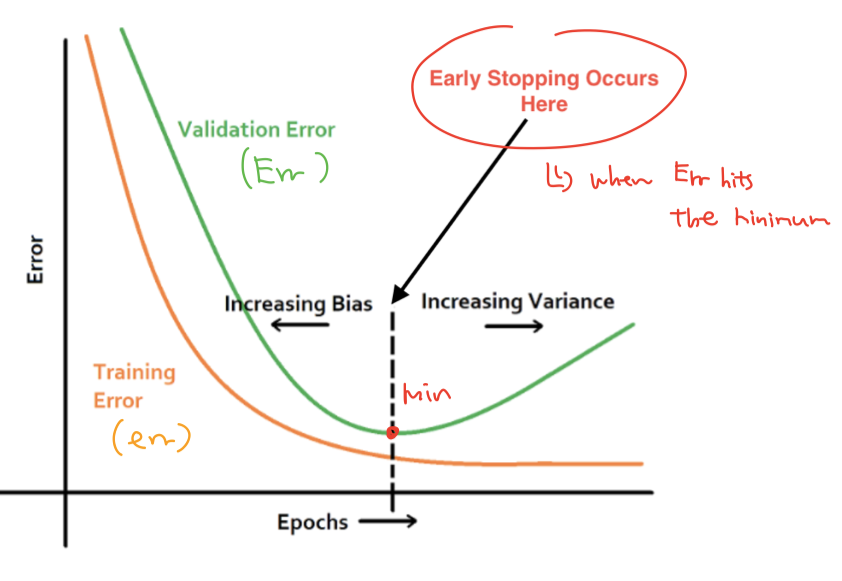
\includegraphics[width=300px]{Figs/Lec6/early-stop}
	
	\begin{enumerate}
		\item Pick a model M
		\item Run the training and validation at the same time \\
			(Validation uses the model that was just trained in the most recent iteration)
		\item At certain point, the \blue{validation set} is \blue{not improving} in terms of low error performance, while \red{training error} keeps \red{decreasing}.
		\item Stop the training and pick the model that led to the lowest validation error
	\end{enumerate}
	
	- Repeat the process with different models (different number of nodes or different regression parameters) and get the lowest possible error. 

	- The model leads to the lowest training and validation error is the one to choose from.
\end{remark}

\begin{remark}[Cross Validation]{r6:cross-validation}
	The model may contain some \red{hyper-parameters} which need to be optimized without using the test data during training. \textbf{Validation Dataset} is used for this.
	
	- \textbf{Cross Validation} divides the full training data into $k$ equal portions, taking on portion for validation while the rest is used for training. 
	
	- The portion is moved and finally the model is re-trained by the parameters with best validation performance.
	
	The well-known types are:
	\begin{itemize}
		\item $K$-fold cross validation [\Cref{r6:K-fold}]
		\item Leave-one-out cross validation
	\end{itemize}
\end{remark}

\begin{remark}[$K$-fold Cross Validation]{r6:K-fold}
	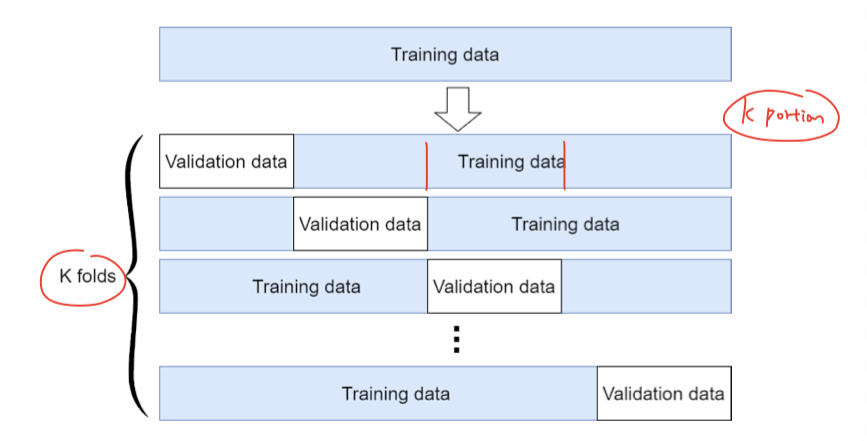
\includegraphics[width=350px]{Figs/Lec6/k-fold}
	
	The \red{validation error} is the \red{average} of the errors in each fold.
	
	To build an adequate model while making use of the K-fold validation, proceed as follows:
	
	\begin{enumerate}
		\item Choose the type of model M you want to test: linear regression, polynomials, \Gls{ANN} with different hidden nodes
		\item For each model M, run K-fold validation and average out the validation error among all K folds. \red{Run this operation several times} to ensure the data is well mixed and \red{there is no memorization}.
		\item Change the mode type/parameters and record the results with the K-fold validation. Check again the validation errors for each model.
		\item The model with the smallest validation error is selected. Now train it with all the training data you have, and finally test it with testing data, for which the system never saw.
	\end{enumerate}
\end{remark}

\begin{note}[More References to Read About under/over-fitting]{pink}{note6:extra}
	\begin{itemize}
		\item \uhref{Idea [Youtube]}{https://www.youtube.com/watch?v=BqzgUnrNhFM}
		\item \uhref{Theory [Youtube}{https://www.youtube.com/watch?v=nqtfl137jio}
		\item \uhref{Cross-validation [Youtube]}{https://www.youtube.com/watch?v=7062skdX05Y}
		\item \uhref{Overfitting [Tut Paper]}{https://arxiv.org/pdf/1905.12787.pdf}
		\item \uhref{Early Stopping [Reading]}{https://machinelearningmastery.com/early-stopping-to-avoid-overtraining-neural-network-mo}
	\end{itemize}
\end{note}

\begin{note}[Summary: Generally Speaking]{pink}{alert6:final}
	\begin{itemize}
		\item Under-fitting (high bias) occurs when the training data is not enough or / and when the model is too simple (smaller number of nodes in ANN or linear or first order polynomials regressors). \red{Hence, increase the training data and increase complexity of the model gradually until good testing results are provided}.
		\item Overfitting (high variance) occurs when the model selected (ANN or high degree polynomials) is too complex, and the training data is not enough to describe the entire population (leads to poor testing results). Overfitting also occurs when there are too many iterations (stop training when the validation/test error starts increasing). \red{Reduce complexity of the model gradually while keeping good amount of training data}.
	\end{itemize}	
	
	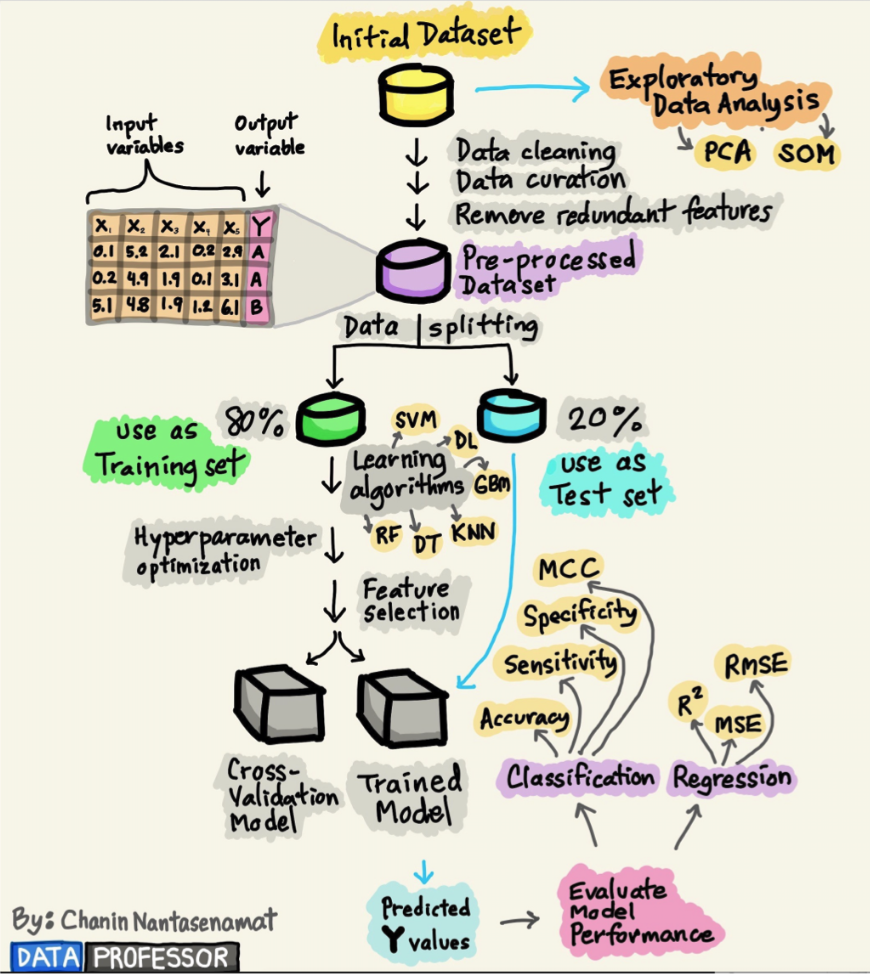
\includegraphics[width=400px]{Figs/Lec6/of-uf}
\end{note}


\newpage
%%%%%%%%%%%%%%%%%%%%%%%%%%%%%%%%%%%%%%%%%%%%%%%%%%%%%%%%%%%%
%%%% Slide 7 - Performance Measures for Classification %%%%%
%%%%%%%%%%%%%%%%%%%%%%%%%%%%%%%%%%%%%%%%%%%%%%%%%%%%%%%%%%%%
\section{Performance Measures}
%%%% Performance Measres
\subsection{Performance Measures for Classification}
\vspace{5pt}
\begin{remark}[True/False Positive/Negatives]{r7:tfpn}
	Consider a binary classification (positive and negative classes):
	
	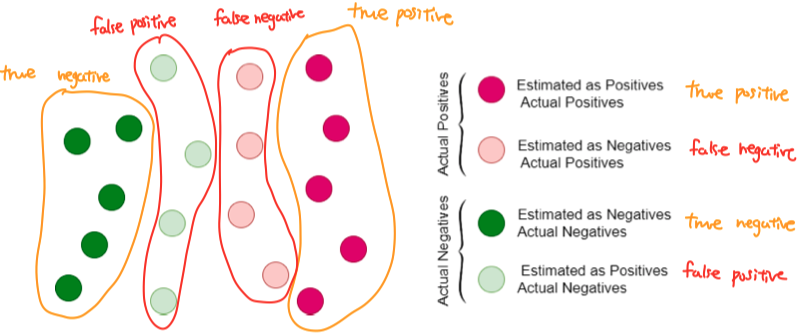
\includegraphics[width=450px]{Figs/Lec7/tfpn}
	
	Every prediction of the model belongs to one of following categories:
	\begin{itemize}
		\item \textbf{\blue{True Positive (TP)}}: predicted as positive and the estimation is correct (it is actually in positive class)
		\item \textbf{\blue{True Negative (TN)}}: predicted as negative and the estimation is correct (it is actually in negative class)
		\item \red{\textbf{False Positive (FP)}}: predicted as positive and the estimation is wrong (it is actually in negative class)
		\item \red{\textbf{False Negative (FN)}}: predicted as negative and the estimation is wrong (it is actually in positive class)
	\end{itemize}
\end{remark}

\begin{definition}[Confusion Matrix]{def7:confusion-mat}
	The confusion matrix is a table which is formed from the four outcomes of a binary classification (class 1 is positive and class 0 is negative) which is later used to easily calculate different metrics.
	
		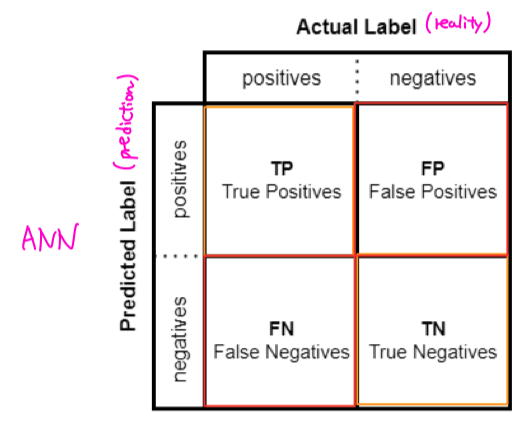
\includegraphics[width=260px]{Figs/Lec7/conf-mat}
\end{definition}

\begin{definition}[Accuracy]{def7:accuracy}
	Accuracy measures what ratio of points have been correctly estimated/classified.
	\begin{eqn}[Accuracy]{}
		\textbf{Accuracy} = \frac{\text{Correct Predictions}}{\text{All Classes}} = \frac{TP + TN}{TP + TN + FP + FN}
	\end{eqn}
\end{definition}

\begin{definition}[Precision and Recall]{def7:precision-recall}
	Precision measures what ratio of estimations as a class are correct \blue{among all points estimated as that class}.
	\begin{eqn}[Precision]{}
		\textbf{Precision} = \frac{\text{True Positives}}{\text{All Predicted Classes as Positive}} = \frac{TP}{TP + FP}
	\end{eqn}	
	Recall measures what ratio of estimations as a class are correct \blue{among all points that actually belong to that class}.
	\begin{eqn}[Recall]{}
		\textbf{Recall} = \frac{\text{True Positives}}{\text{All Actual Positive Classes}} = \frac{TP}{TP + FN}
	\end{eqn}
\end{definition}

\begin{definition}[$F_{\beta}$ Score]{def7:Fbeta}
	The $F_{\beta}$ score measures \red{whether both precision and recall are good enough}, i.e., whether truly estimated points as a class are a big percentage among both all estimated points as that class and all actual points of that class.
	\begin{eqn}[$F_{\beta}$ Score]{}
		F_{\beta} = (1+ \beta^2) \times \frac{\text{Precision} \times \text{Recall}}{(\beta^2 \times \text{Precision}) + \text{Recall}}
	\end{eqn}
	\begin{eqn}[A well-known value for $\beta = 1$]{}
		F_1 = 2 \times \frac{\text{Precision} \times \text{Recall}}{\text{Precision} + \text{Recall}}
	\end{eqn}
\end{definition}

\begin{definition}[TPR and FPR Rates]{def7:TPR-FPR}
	TPR (\textbf{True Positive Rate}) and FPR (\textbf{False Positive Rate}) are defined as:
	\begin{eqn}[TPR]{}
		\textbf{TPR} = \textbf{Recall} = \frac{\text{True Positives}}{\text{All Actual Positive Classes}} = \frac{TP}{TP + FN}
	\end{eqn}
	\begin{eqn}[FPR]{}
		\textbf{FPR} = \frac{\text{False Positives}}{\text{All Actual Negative Classes}} = \frac{FP}{FP + TN}
	\end{eqn}
\end{definition}

\begin{remark}[Other Performance Metrics]{r7:other-metrics}
	\textbf{Error Rate}: Ratio of incorrect predictions to total number of samples:
	\begin{eqn}[Error Rate]{}
		\textbf{ERR} = 	 \frac{FP + FN}{TP + TN + FP + FN}
	\end{eqn}
	\textbf{Specificity}: Proportion of negative data points that are correctly classified as negative (True Negative Rate - TNR).
	\begin{eqn}[Specificity]{}
		\textbf{SP} = 	 \frac{TN}{TN + FP}
	\end{eqn}
\end{remark}

\begin{definition}[POC and AUC]{def7:poc-auc}
	The curve of \blue{TPR vs. FPR} is the \red{ROC} (Receiver Operating Characteristic) curve, We have a curve by sweeping on the threshold of classification.
	
	AUC (Area Under Curve) is the area under ROC curve ($0 \leq AUC \leq 1$).
	
	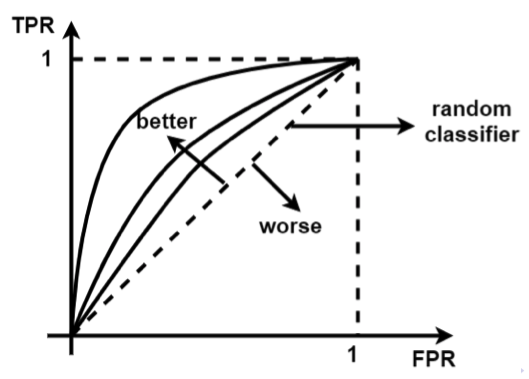
\includegraphics[width = 250px]{Figs/Lec7/roc-curve}
\end{definition}

\begin{remark}[Multi-Class Confusion Matrix]{r7:multi-class}
	When we have more than 2 classes, the points are classified to one of the classes. These points have actual class labels, too. The table of estimated labels versus actual labels creates the multi-class confusion matrix. Every column sums to 100\%. 
	
	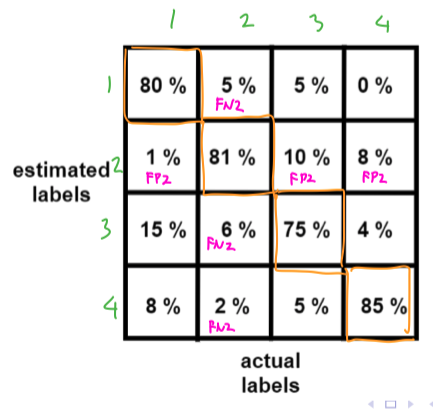
\includegraphics[width = 250px]{Figs/Lec7/multi-class-conf-mat}
\end{remark}

%%%% Examples
\newpage
\subsection{Examples for Measuring Classification Performance}
\vspace{5pt}

\begin{example}[Comparing Models]{}
	Assume a model (A) that classifies emails to be either spam (C1) or non-spam (C2). After testing the model, the following confusion matrix was created. Calc the accuracy of the model.
	
	Another model (B) was trained and tested on the same dataset. Calculate the accuracy and deduce which model is better.
	
	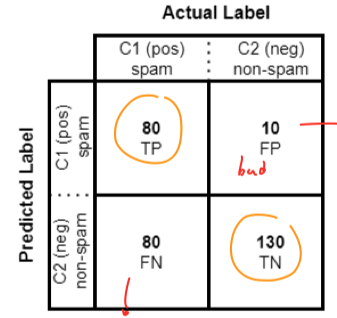
\includegraphics[width = 200px]{Figs/Lec7/ex1-a}
	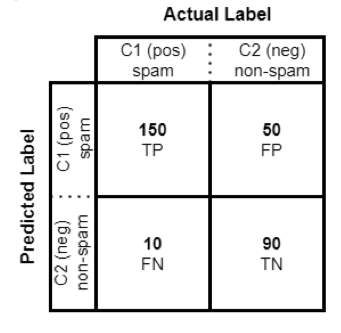
\includegraphics[width = 200px]{Figs/Lec7/ex1-b}
	
	\begin{align}
		\text{Accuracy}_A & = \frac{TP + TN}{TP + TN + FP + FN} = \frac{80 + 130}{300} = 70 \% \\
		\text{Accuracy}_B & = \frac{150 + 90}{300} = 80 \% 
	\end{align}
	
	
	You may intuitively think that Model B is better than model A. However, lets compare their other metrics to understand the performance:
	
	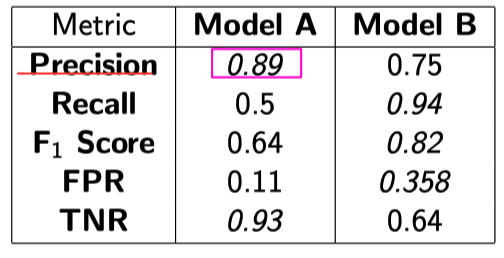
\includegraphics[width = 200px]{Figs/Lec7/ex1-table}
	
	As a result, we may conclude:
	\begin{itemize}
		\item Precision: Model A is likely to mark and email as spam and be wrong, but is more likely to miss a spam email.
		\item TNR: Model A is better at detecting non-spam email than Model B. Note that this can be due to simply marking all as non-spam (bias).
		\item Recall: Model B is better at marking emails that are spam as spam than Model A.
	\end{itemize}
	
	hence, we deduce that the choice of model depends on what kind of performance is favourable to the use-case.
\end{example}

\begin{example}[Actual and Predicted Labels]{}
	Consider a classification problem for whether a person, in a population of 10 people, is tested as infected (+ve) or not (-ve).
	
	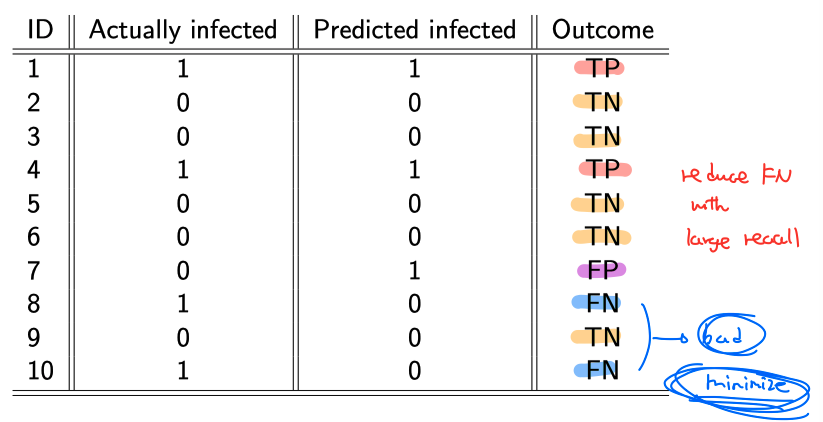
\includegraphics[width = 250px]{Figs/Lec7/ex2-table}
	
	Confusion Matrix:
	
	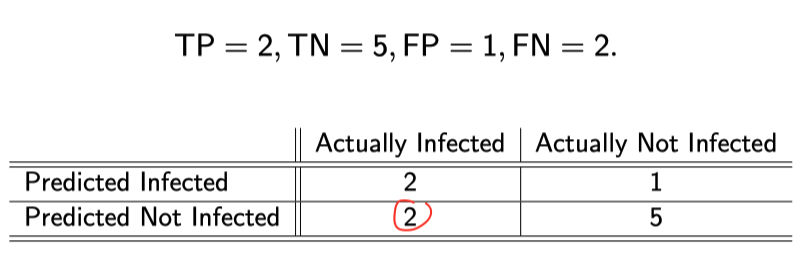
\includegraphics[width = 250px]{Figs/Lec7/ex2-conf-mat}
	
	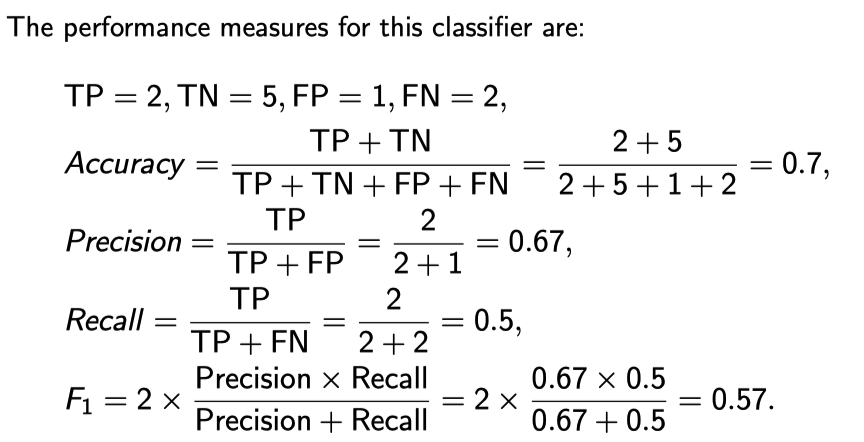
\includegraphics[width = 300px]{Figs/Lec7/ex2-perform measure}
	
	Comments:
	\begin{itemize}
		\item While Accuracy (0.7) and Precision (0.67) are relatively high, this is not a good classifier for this particular example
		\item The fact that the system is not able to catch an infected person twice (two FN) shows this is not a good classifier. One non-caught infected person, could transmit the virus to others without their knowledge (especially if no symptoms appear early on).
		\item The $F_1$ measure always takes a value between the Recall and Precision, with tendency towards the lower among either one. This is due to the fact that the $F_1$ measure is the harmonic average of both values.
	\end{itemize}	
\end{example}


\begin{example}[Multi-Class Classification]
	You created a model capable of classifying images of dogs into one of three breeds: Golden Retriever, Samoyed, and Mastiff. After testing the model, the following confusion matrix was created.
	
	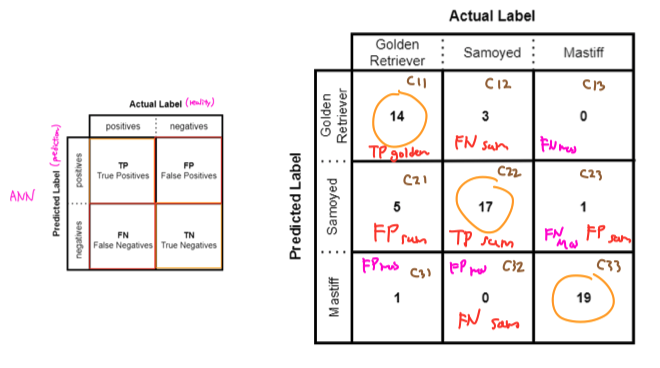
\includegraphics[width = 300px]{Figs/Lec7/ex3-mat}
	
	To calculate various performance metrics, the TP, FP, TN, and FN have to be calculated for each label.
	Assume $C_{ij}$ stands for cell in row i and column j:
	
	\includegraphics[width = 350px]{Figs/Lec7/ex3-table}	
	
	Therefore, we end up with the following values:
	
	\includegraphics[width = 250px]{Figs/Lec7/ex3-table2}	
	
	These values can then be used to calculate the rest of the measures either in a one-vs-all (per-class) or all-vs-all (using the population as a whole by summing the TP, FP, TN, and FN values).
	
	\begin{example}[One-vs-all]{}
		We show computation for one of the classes (Golden Retriever). Other classes are processed similarly. Total measures are the avg. rates over all the classes. 
	
	\includegraphics[width = 300px]{Figs/Lec7/ex3-one-vs-all}
	\end{example}

	\begin{example}[All-vs-all]{}
	We sum all TPs, FPs, and FNs to find: TP = 50, FP = 10, FN = 10
	
	\includegraphics[width = 300px]{Figs/Lec7/ex3-all-vs-all}
	
	Note: all measures become equal when we do "all-vs-all"
	\end{example}	
\end{example}


%%%% Regression
\newpage
\subsection{Performance Measures for Regression}
\vspace{5pt}

\begin{definition}[MSE (Mean Squared Error)]{def7:mse}
	\begin{center}
		\includegraphics[width = 300px]{Figs/Lec7/mse}
	\end{center}

	\textbf{MSE} measures error where the high errors where the high errors get \red{bold} because of the power 2. 
	
	$\Rightarrow (Outliner)^2 \rightarrow \textbf{Even Larger}$
	
	Treat +ve and -ve terms equally.
	
	\begin{eqn}[MSE]{eqn:mse}
		MSE = \frac1n \sum_{i=1}^n (y_i - \hat{y}_i)^2		
	\end{eqn}

	
	\textbf{RMSE} (Root MSE) measures the error in the original scale of the quantity:
	\begin{eqn}[RMSE]{eqn:rmse}
		RMSE = \sqrt{\frac1n \sum_{i=1}^n (y_i - \hat{y}_i)^2}
	\end{eqn}
\end{definition}

\begin{definition}[MAE (Mean Absolute Error)]{def7:MAE}
	\begin{center}
		\includegraphics[width = 150px]{Figs/Lec7/mae}
	\end{center}

	\textbf{MAE} measures error which is \blue{more robust to outliers} than MSE because it does not have power 2. (L1 norm vs. L2 norm)
	
	\begin{eqn}[MAE]{eqn:mae}
		MAE = \frac1n \sum_{i=1}^n | y_i - \hat{y}_i |
	\end{eqn}
\end{definition}


\begin{definition}[MedianAE (Median Absolute Error)]{def7:MedianAE}
	\begin{center}
		\includegraphics[width = 300px]{Figs/Lec7/medianae}
	\end{center}

	\textbf{MedianAE} measures error which is \blue{robust to outliers} because of median operator rather than mean.
	
	\begin{eqn}[MedianAE]{eqn:medianae}
		MAE = \text{median}\{ |y_1 - \hat{y}_1| , \dots , |y_n - \hat{y}_n| \}
	\end{eqn}
\end{definition}

\begin{definition}[$R^2$ Score]{def7:R2-score}
	\begin{center}
		\includegraphics[width = 150px]{Figs/Lec7/mae}
	\end{center}

	\textbf{$R^2$ Score} is similar to MSE but normalizes with the error from the mean of data.
	
	\begin{eqn}[MedianAE]{eqn:medianae}
		R^2 = 1 - \frac{\frac1n \sum_{i=1}^n (y_i - \hat{y}_i)^2	}{\frac1n \sum_{i=1}^n (y_i - \bar{y}_i)^2	}, \quad \text{with} \quad \bar{y} = \frac1n \sum_{i=1}^n y_i	
	\end{eqn}
\end{definition}

\begin{note}[More References to Read About Performance]{pink}{note7:extra}
	\begin{itemize}
		\item \uhref{Measures Summary [Python]}{https://scikit-learn.org/stable/modules/model_ evaluation.html}
		\item \uhref{Confusion Matrix [Web]}{https://www.analyticsvidhya.com/blog/2020/04/confusion-matrix-machine-learning/}
	\end{itemize}
\end{note}


\newpage
%%%%%%%%%%%%%%%%%%%%%%%%%%%%%%%%%%%%%%%%%%%%
%%%% Slide 8 - Support Vector Machines %%%%%
%%%%%%%%%%%%%%%%%%%%%%%%%%%%%%%%%%%%%%%%%%%%
\section{Support Vector Machines \Gls{SVM}}
%%%% The Kohonen's Self-Organizing Network
\subsection{Introduction}
\begin{remark}[SVM]{}
	\begin{itemize}
		\item SVM is a \red{kernel-based classifier}
		\item Originated from the theoretical foundations of \red{Statistical Learning Theory (SLT)} and \red{Structural Risk Minimization (SRM)}
		\item Unlike classical approaches to minimize \blue{L1 or L2 norm of error}, SVMs perform SRM to find a model with minimal \red{VC dimension}
		\item SVM learns during training process and \red{generalizes} to new data
		\item data is \red{labeled}: $D = \{(\xv_1,y_1), \dots , (\xv_m,y_m) \in \mathbb{R}^{N} x Y \}$
	\end{itemize}
\end{remark}

%%%% The Hop field Network
\subsection{Theory}
\begin{remark}[SVM: Basic Idea]{}
	\includegraphics[width=200px]{Figs/slide8/svm-basic}
	
	\begin{itemize}
		\item SVM use \red{kernel} to map data point vectors $\xv_i$ to vectors $\phi (\xv_i)$ in a higher-dimensional feature space
		\item Each $\phi (\xv_i)$ belongs to the \red{same group} $y_i$ as $x_i$ does
		\item In the feature space, the vectors are \red{linearly separable}
		\item SVM obtains a \red{hyper-plane} $f(x) = \inner{w}{\phi(x)} + b = 0$, which intersects with the manifold in the feature space to generate the decision function in the input space/
		\item By using a \red{kernel}, SVM does not directly work in the feature space which would be computationally expensive.
	\end{itemize}
\end{remark}

\clearpage
%%%% Hard Margin
\subsection{Hard Margin SVM (Original)}
\begin{definition}[Hard Margin SVM]{}
	\includegraphics[width=300px]{Figs/slide8/svm-hard}
	
	\begin{itemize}
		\item Margin M: \red{shortest distance} from the discriminant hyper-plane to the closest samples from each class (support vectors), which lie on $\wv^T \xv + b = 0$.
			\begin{equation}
			M = \frac{|1-b|}{\|\wv\|} - \frac{|-1-b|}{\|\wv\|} = \frac{2}{\|\wv\|}
			\end{equation}
		\item For the linearly separable case, the support vector algorithm simply looks for the separating hyper-plane with \red{largest} margin
		\item Thus, \red{maximizing} M translates to \red{minimizing} $\wv$, or for mathematical convenience, $J(\wv) = \frac12 \wv^T \wv$ subject to: 
			\begin{equation}
				y_i (\wv^T \xv_i + b) \geq 1, \, i=1,\dots,l
			\end{equation}
		\item Hence, we are dealing with a classic quadratic programming (QP) optimization problem:
			\begin{equation}
				J(\wv) = \frac12 \wv^T \wv
			\end{equation} 
			 with \red{inequality constraints}: 
			 \begin{equation}
			 	y_i(\wv^T \xv_i + b) \geq 1, \, i = 1, \dots, l
			 \end{equation}
		\item Reformulating the problem with Lagrange Multiplier, yield:
		\begin{equation}
			L(\wv, b, \alpha) = \frac12 \wv^T \wv - \sum_{i=1}^l \alpha_i \left[ y_i (\wv^T \xv_i + b) - 1 \right]
		\end{equation}	
		\item The optimal saddle point $(w_o, b_o, \alpha_o)$ can be found using \red{Karush Kuhn Tucker (KKT) conditions} for $\alpha_i \geq 0, i = 1, \dots , l$:
		\begin{align}
			\frac{\partial L}{\partial \wv_o} = 0 & \rightarrow \wv_o = \sum_{i=1}^l \alpha_i y_i \xv_i \\
			\frac{\partial L}{\partial b_o} = 0  & \rightarrow \sum_{i=1}^l \alpha_i y_i = 0
		\end{align}
		\item Now we may obtain the \red{\textbf{dual form}}:
		\begin{align}
			& L_d(\alpha) = \sum_{i=1}^l \alpha_i - \frac12 \sum_{i, j=1}^l y_i y_j \alpha_i \alpha_j \xv_i^T \xv_i \\
			& \textbf{such that:}\\
			& \sum_{i=1}^l \alpha_i y_i = 0 \quad \alpha_i \geq 0 \, \forall i = 1, \dots, l
		\end{align}
	\end{itemize}
	
	\begin{eqn}[Final Solution with any of the \blue{standard optimization programs}]{}
	\begin{split}
		 & \wv_o = \sum_{i=1}^l \alpha_o y_i \xv_i  \\
		 & b_o = \frac1{N_{sv}} \left( \sum_{s=1}^{N_{SV}} \left( \frac1{y_s} - \xv_s^T \wv_o \right) \right)\quad \forall s \in \{1, \dots, N_{SV}\}
	\end{split}
	\end{eqn}
\end{definition}

\clearpage

%%%% Soft Margin
\subsection{Soft Margin SVM}
\begin{definition}[Soft Margin SVM]{}
	\includegraphics[width=400px]{Figs/slide8/svm-soft}
	
	\begin{itemize}
		\item Optimization problem is updated to include \red{slack variables} $\zeta_i$:
			\begin{equation}
				J(\wv) = \frac12 \wv^T \wv + \blue{C} \sum_{i=1}^l \zeta_i
			\end{equation}
			with \red{inequality constraints}:
			\begin{equation}
				y_i(\wv^T \xv_i + b) \geq 1\red{- \zeta_i}, \, i = 1, \dots, l\, \zeta_i \geq 0
			\end{equation}
		\item Soft-margin SVM uses an error cost parameter \blue{C} to address \red{misclassification} issue
		\item As \blue{C} \red{$\uparrow$} $\Rightarrow$ \red{the tolerance} \red{$\downarrow$} for \red{misclassification} of the vectors by the optimal hyperplane and a \blue{more accurate} but \red{less generalizing} optimal hyper-plane is obtained, and vice versa.
		\item \textbf{Primal Problem}:
		\begin{align}
			& L_d(\alpha) = \sum_{i=1}^l \alpha_i - \frac12 \sum_{i, j=1}^l y_i y_j \alpha_i \alpha_j \xv_i^T \xv_i \\
			& \textbf{such that:}\\
			& \sum_{i=1}^l \alpha_i y_i = 0 \quad \blue{C \geq} \alpha_i \geq 0 \, \forall i = 1, \dots, l
		\end{align}
		\item The only difference is the  \blue{upper bound C} on Lagrange multipliers to control \red{overfitting}
		\item \textbf{Primal Form}:
		\begin{equation}
			L(\wv, b, \alpha) = \frac12 \wv^T \wv \blue{+ C \sum_{i=1}^n \zeta_i}- \sum_{i=1}^l \alpha_i \left[ y_i (\wv^T \xv_i + b) - 1 \blue{+ \zeta_i}\right] \blue{ - \sum_{i=1}^n \beta_i \zeta_i} \quad \alpha_i,\beta_i \geq 0 \forall i \in \{1, \dots, n\}
		\end{equation}	
		\item KKT conditions, derive the \textbf{Dual Form}:
		\begin{align}
			& L_d(\alpha) = \sum_{i=1}^l \alpha_i - \frac12 \sum_{i=1}^l\sum_{j=1}^l \alpha_i \alpha_j y_i y_j K(\xv_i, \xv_j) \\
			& \textbf{such that:}\\
			& \sum_{i=1}^l \alpha_i y_i = 0 \quad \blue{C \geq} \alpha_i \geq 0 \, \forall i = 1, \dots, l
		\end{align}
	\end{itemize}
	
	\TODO{Checkout derivation from CS480 Notes}
	
	\begin{eqn}[Final Solution with any of the \blue{standard optimization programs}]{}
		\begin{split}
			 & \wv_o = \sum_{i=1}^l \alpha_o y_i \xv_i \\
			 & b_o = \frac1{N_{sv}} \left( \sum_{s=1}^{N_{SV}} \left( \frac1{y_s}\blue{1-\zeta_s} - \xv_s^T \wv_o \right) \right)\, s = 1, \dots, N_{SV} \\
			 & \text{with decision function:}\\
			 & f(x) = \sum_{i=1}^n \alpha_i y_i K(\xv_i, \xv) + b			
		\end{split}
	\end{eqn}
\end{definition}

\clearpage
%%%% Non-linear: Kernels
\subsection{Kernels: Non-linear SVM}
\begin{definition}[Non-linear Margin SVM : Kernels]{}
	\includegraphics[width=400px]{Figs/slide8/svm-nonlinear}
	
	\begin{itemize}
		\item There might be cases in which the given dataset is \red{not linearly separable} using discriminant functions, hence, we may map the data to \red{high-er-dimensional feature space}, along with using \red{kernel} trick for dot product in that space.
		\item Linear SVM relies on \red{dot product} between two vectors $x_i$ and $x_j$ that might become an \red{unmanageable} operation in \red{high-dimensional} data after mapping
		\item A kernel function $K(\xv_i,\xv_j)$ provides this dot product while \red{implicitly mapping} the data points to higher-dimensional feature space
	\end{itemize}
	
	\begin{example}[]{}
		\begin{align}
			 & K(\xv_1, \xv_2) = (1 + \xv_1^T \xv_2) = \Phi(\xv_i) \Phi(\xv_j) \\
			 & \textbf{where: } \Phi(x) = [1, \xv_i^2, \sqrt2 \xv_i\xv_j, \xv_j^2, \sqrt2 \xv_i, \sqrt2 \xv_j]
		\end{align}
	\end{example}

	\begin{theorem}[Kernel]{}
		A kernel is a \red{real-valued function} $K(\xv_1, \xv_2)$ satisfy Mercer's condition:
		
		There exists a \red{mapping $\Phi$} and an expansion:
		\begin{equation}
			K(\xv_1, \xv_2) = \sum_i \Phi(\xv_1)_i \Phi(\xv_2)_i
		\end{equation}
		
		If and only if for any $g(\xv)$, such that $\int g(\xv)^2 d\xv$ is \red{infinite} then:
		\begin{equation}
			\int K(\xv_1, \xv_2) g(\xv_1) g(\xv_2) d\xv_1 d\xv_2 \geq 0
		\end{equation}
	\end{theorem}
	
	\begin{example}[Commonly Used Kernels]{}
		\begin{align}
			\textbf{Linear} \quad & K(\xv_1, \xv_2) = \xv_1^T \xv_2 \\
			\textbf{Polynomial} \quad & K(\xv_1, \xv_2; c, d) = (c + \xv_1^T \xv_2)^d \\
			\textbf{RBF (Radial-Basis Function)} \quad & K(\xv_1, \xv_2; \sigma) = \exp\left(- \frac1{\sigma^2} \|\xv_1 - \xv_2\|^2 \right) \\
			\textbf{Sigmoid} \quad & K(\xv_1, \xv_2; \alpha, c) = \tanh (\alpha \xv_1^T \xv_2 + c)
		\end{align}
				
		\begin{center}
		\includegraphics[width=300px]{Figs/slide8/svm-kernel-ex}
		\end{center}

		\textbf{More:}
				
		1. Linear Kernel
		14. Power Kernel
		2. Polynomial Kernel
		15. Log Kernel
		3. Gaussian Kernel
		16. Spline Kernel
		4. Exponential Kernel
		17. B-Spline Kernel
		5. Laplacian Kernel
		18. Bessel Kernel
		6. ANOVA Kernel
		19. Cauchy Kernel
		7. Hyperbolic Tangent (Sigmoid) Kernel
		20. Chi-Square Kernel
		8. Rational Quadratic Kernel
		21. Histogram Intersection Kernel
		9. Multiquadric Kernel
		22. Generalized Histogram Intersection Kernel
		10. Inverse Multiquadric Kernel
		23. Generalized T-Student Kernel
		11. Circular Kernel
		24. Bayesian Kernel
		12. Spherical Kernel
		25. Wavelet Kernel
		13. Wave Kernel

	\end{example}
	
	\begin{remark}[Kernels Properties]{}
		\begin{itemize}
			\item Global kernels such as the \textbf{linear kernel} give a \red{good prediction} ability 
			\item local kernels such as the \textbf{RNF kernel} give a \red{good learning} ability
			\item Every \red{semi-positive definite symmetric} function is a kernel which can be linearly combined
			\item Kernels can be combined to take advantage of their properties
			\item For instance, \red{CombKer} that is a combination of linear and RBF kernels:
			\begin{equation}
				K(\xv_i, \xv_j) = (1-\lambda)\inner{\xv_i}{\xv_j} + \lambda \exp \{ -\gamma \times \| \xv_i - \xv_j \|^2 \}
			\end{equation}
			 As a result, it has both \red{good prediction ability} from \red{linear kernel} (global kernel) and \blue{good learning ability} inherited from \blue{RBF kernel} (local kernel)
		\end{itemize}
	\end{remark}
\end{definition}

%\clearpage
%%%% Non-linear: Kernels
\subsection{Fuzzy SVM}
\begin{definition}[Fuzzy SVM]{}
	\includegraphics[width=200px]{Figs/slide8/svm-fuzzy}
	
	\begin{itemize}
		\item Same as hard-margin SVM
		\item Difference: Fuzzy \red{membership functions} are defined for data points near the boundary:
		\begin{itemize}
			\item $i = j : m_{ij}(x) = \begin{cases} 1 & \forall D_j(\xv) > 1 \\  D_j(\xv) & \text{else}\end{cases}$
			\item $m_i(\xv) = \min_{j=1\dots k} m_{ij} (\xv)$ 
			\item Class label: $\argmax_{i=1\dots k}m_i(\xv)$
		\end{itemize}
	\end{itemize}
\end{definition}

\newpage
%%%% Properties / Summary
\subsection{Summary}
\begin{itemize}
	\item SVMs provide a powerful and flexible approach to \red{learn discriminant/approximating functions} in pattern recognition tasks
	\item Extensions to SVMs allow for dealing with \red{noisy, overlapping, and complex} data
	\item Further research required on choice of \red{Kernel functions} and direct formulization of multi-class SVMs
	\item Much exciting research is ongoing to improve SVM. Some of the latest research topics include \red{fuzzy SVM, genetic kernel SVM and hybridizing SVM} with other soft-computing techniques such as using the \red{genetic algorithm} for initializing its parameters
	\item New applications of SVMs such as \red{data fusion} and density estimation are emerging
\end{itemize}

\subsubsection{Pros and Cons}
\begin{remark}[Pros and Cons of SVM]{}
Pros:
\begin{itemize}
	\item Flexible choice of similarity function
	\item well-founded theoretical approach to regularization
	\item SVM has sparseness and convexity properties
	\item SVM uses kernels to obtain complex decision functions
	\item SVM is able to tolerate misclassification
	\item Resolves overfitting through soft margin approach
\end{itemize}

Cons:
\begin{itemize}
	\item Choice of kernel function is crucial
	\item SVM is vulnerability to incorrectly labeled training data
	\item SVM is rather sensitive to noise
	\item SVM has high computational complexity in the case of multi-class data
	\item Although SVM has good generalization performance, it can be awfully slow in test phase
\end{itemize}	
\end{remark}


\newpage
%%%% Application
\subsection{Application}
\begin{example}[SVM Applications]{}
\begin{itemize}
	\item Isolated Handwritten Digit Recognition
	\item Object Recognition
	\item Speaker Identification
	\item Bioinformatics
	\item Charmed Quark Detection
	\item Face Detection in Images 
	\item Text Categorization
	\item Regression Estimation
	\item Time Series Prediction Tests
	\item Boston Housing Problem
	\item PET Operator Inversion Problem
	\item Support Vector Clustering (SVC)
\end{itemize}
\end{example}

\subsubsection{TODO: Support Vector Clustering} 
\begin{remark}[Outline of the approach]{}
– In data space, a transformation function is used to map the data points to a high-dimensional space (called feature space)

– In feature space, a hyper sphere with minimum radius is found that encloses a set of data points

– In data space, a set of contours are formed by mapping back the hyper sphere

– In data space, data points within each contour are associated with the same cluster
\end{remark}
\TODO{To be added from slides (pg. 35 - 45)}



\newpage
%%%%%%%%%%%%%%%%%%%%%%%%%%%%%%%%%%%%%%%%%%%%%%%%%%%%%%%%%%%%%%
%%%% Slide 9 - Unsupervised and Associative Memory Based %%%%%
%%%%%%%%%%%%%%%%%%%%%%%%%%%%%%%%%%%%%%%%%%%%%%%%%%%%%%%%%%%%%%
\section{Unsupervised and Associative Memory Based}
%%%% The Kohonen's Self-Organizing Network
\subsection{Unsupervised Learning: The Kohonen's Self-Organizing Network}
%%%% %%%% Topology
\subsubsection{Topology}
	\begin{itemize}
		\item The Kohonen’s Self-Organizing Network ( KSON ) also called The Kohonen’s Self-Organizing Map ( KSOM ) belongs to the class of \red{unsupervised learning networks}.
		\item This means that the network, unlike supervised learning based networks updates its weighting parameters without the need for a performance feedback from a teacher or a network trainer.
		\item One major feature: the nodes distribute themselves across the input space to recognize groups of similar input vectors.
		\item Instead, using \textbf{Competitive Learning}: The output nodes compete among themselves to be fired one at a time in response to a particular input vector
		\item Two input vectors with similar pattern characteristics excite two physically close layer nodes $\Rightarrow$ the nodes of the KSON can recognize groups of similar input vectors.
		\item This generates a topographic mapping of the input vectors to the output layer, which depends primarily on the pattern of the input vectors and results in dimensionality reduction of the input space.
	\end{itemize}
	
	\begin{figure}[H]
	\center
		\includegraphics[width=350px]{Figs/KSON/KSOM}
	\end{figure}

%%%% %%%% Learning
\subsubsection{Learning Algorithm}
\begin{itemize}
	\item The learning here permits the clustering of input data into a smaller set of elements having similar characteristics (features)
	\item It is based on the competitive learning technique also known as the \red{winner take all} strategy
	\item Presume that the input pattern is given by the vector $\xv$
	\item Assume $w_{ij}$ is the weight vector connecting the input elements to an output node with coordinate provided by indices $i$ and $j$.
	\item $N_c$: neighborhood around the winning output candidate, decreases at every iteration of the algorithm until convergence occurs
\end{itemize}

\begin{algo}[KOSM Steps]{}
	\begin{enumerate}
		\item Initialize \textbf{all weights} to small random values, set a value for the initial \textbf{learning rate} $\alpha$ and a value for the \textbf{neighborhood} $N_c$.
		\item Choose an input pattern $x$ from the input dataset
		\item Select the winning unit $c$ (the index of the best matching output unit) such that the performance index $l$ given by the Euclidian distance from $x$ to $w_{ij}$ is minimized: $l = \| x - w_c \| = \min_{ij}\| x - w_{ij}\|$
		\item Update the weights according to the global network updating phase from iteration $k$ to iteration $k+1$ as:
		\begin{equation}
			w_{ij}(k+1) = 
			\begin{cases}
				w_{ij}(k) + \alpha(k) [x - w_{ij}(k)] & \text{if} \, (i,j)\in N_c(k) \\
				w_{ij} & \text{otherwise}
			\end{cases}
		\end{equation}
		\begin{eqconditions}
			\alpha(k) & adaptive learning rate, $\in (0, 1)$ \\
			N_c(k) & neigborhood of the unit $c$ at iteration $k$
		\end{eqconditions}
		\item The learning rate and the neighborhood are decreased $\downarrow$ at every iteration according to an appropriate scheme:
			\begin{itemize}
				\item For instance, Kohonen suggested a shrinking function: $\alpha(k) = \alpha(0) (1 - k/T)$, with $T$ being the total number of training cycles and $\alpha(0)$ the starting learning rate bounded by one
				\item As for the neighborhood, several researchers suggested an initial region with the size of half of the output grid and shrinks according to exponentially decaying behavior
			\end{itemize}
		\item The learning scheme continues until enough number of iterations has been reached or until each output reaches a threshold of sensitivity to a portion of the input space
	\end{enumerate}
\end{algo}

%\TODO{See examples in slides}

\begin{remark}[Applications]{}
	A variety of KSONs could be applied to different applications using the different parameters of the network, which are:
	\vspace{-5px}
	\begin{itemize}
		\item Neighbourhood size
		\item Shape (circular, square, diamond)
		\item Learning rate decaying behavior
		\item Dimensionality of the neuron array (1-D, 2-D, or n-D)
	\end{itemize}
	
	Given heir self-organizing capabilities based on the competitive learning rule, KSONs have been used extensively for clustering applications such as:
	\vspace{-5px}
	\begin{itemize}
		\item Speech recognition
		\item Vector coding
		\item Robotics applications
		\item Texture segmentation
	\end{itemize}
\end{remark}


\begin{note}[More References About KSOM]{pink}{note7:extra}
	\blue{My personal research:}
	\begin{itemize}
		\item \uhref{Self-organizing Maps [Web]}{https://www.cs.hmc.edu/~kpang/nn/som.html}
	\end{itemize}
\end{note}


\newpage
%%%% The Hop field Network
\subsection{Recurrent Topology: The Hop field Network}
\TODO{OPTIONAL*}


\newpage
%%%%%%%%%%%%%%%%%%%%%%%%%%%%%%%%%%%%%%%%%%%%%%%%%%%%%%%%%%%%%%%%%%%%%%%%%%%%%%%%
%% ************************************************************************** %%
%% *                               Chapter 04                               * %%
%% ************************************************************************** %%
%%%%%%%%%%%%%%%%%%%%%%%%%%%%%%%%%%%%%%%%%%%%%%%%%%%%%%%%%%%%%%%%%%%%%%%%%%%%%%%%
\chapter{Deep Learning}
%%%%%%%%%%%%%%%%%%%%%%%%%%%%%%%%%%%
%%%% Slide 10 - Deep Learning %%%%%
%%%%%%%%%%%%%%%%%%%%%%%%%%%%%%%%%%%
\section{Introduction of Deep Learning}
\TODO{TO PUT CONTENT}


\newpage
%%%%%%%%%%%%%%%%%%%%%%%%%
%%%% Slide 11 - CNN %%%%%
%%%%%%%%%%%%%%%%%%%%%%%%%
\section{CNN}
\subsection{Introduction}
\begin{remark}[CNN]{}
	\begin{itemize}
		\item a Deep Learning algorithm that takes in image as input and assign importance to various aspects in the image and be able to differentiate one from the other
		\item “Convolutional networks are simply neural networks that use convolution in place of general matrix multiplication in at least one of their layers.” [Goodfellow et al., 2016]
		\item Takes into account of spatial correlation with neighbour pixels
		\item CNN reduces the images into a form which is easier to process, without loosing features that are critical for a good prediction
	\end{itemize}
\end{remark}

%%%% Layers
\subsection{Layers}
%%%% %%%% Convolutional Layer
\subsubsection{Convolutional Layer}
To generate a feature map of image.
\begin{figure}[H]
	\center
	\subfloat[Methodolgy]{\includegraphics[width=300px]{Figs/CNN/cnn-methodology}}\\
	\subfloat[Example of RGB]{\includegraphics[width=360px]{Figs/CNN/ex}}
\end{figure}

%%%% %%%% Pooling
\subsubsection{Pooling Layer}
\begin{remark}[Types]{}
\begin{itemize}
	\item Max Pooling
	\item Average Pooling
	\item L2-norm pooling
\end{itemize}
\begin{figure}[H]
	\center
	\includegraphics[width=200px]{Figs/CNN/pooling}
	\caption{Pooling}
\end{figure}
\end{remark}

\begin{remark}[Effects]{}
	One might ask whether pooling will loss the information
	
	It is found that it helps in \red{generalizing the CNN by reducing the effects of background noise}
\end{remark}

\begin{remark}[Objectives]{}
\begin{itemize}
	\item Dimensionality reduction
	\item Extracting dominant features
\end{itemize}
	\includegraphics[width=250px]{Figs/CNN/pooling-2}
\end{remark}

\clearpage
%%%% %%%% Dense & Flatterning
\subsubsection{FC (Fully Connected) Layer (Dense \& Flatterning Layer)}
\begin{remark}[Dense \& Flatterning Layer]{}
FC Layer = Flatterning Layer $\rightarrow$ Flatterning Layer

Flatterning Layer:
	\begin{itemize}
		\item Converts data $\rightarrow$ 1D
		\item Prep. data that can be fed to dense layer
	\end{itemize}
	
Dense Layer:
	\begin{itemize}
		\item It connect every neuron in one layer to every neuron in another layer
		\item ONce trained, it can be like classifier
	\end{itemize}
	\includegraphics[width=250px]{Figs/CNN/fc}
\end{remark}



\newpage
%%%% Regularization
\subsection{Regularization}
Goal: to make model generalized and avoid the model over-fitting

%%%% %%%% Dropout
\subsubsection{Dropout}
\begin{itemize}
	\item Dropout is a method to randomly set some activations to 0 (killing or dropping)
	\item Dropout forces the network to explore more ways of learning patterns instead of depending too much on some features
\end{itemize}
\begin{figure}[H]
	\center
	\includegraphics[width=300px]{Figs/CNN/dropout}
	\caption{Dropout}
\end{figure}

%%%% %%%% Batch Norm
\subsubsection{Batch Normalization}
\begin{itemize}
	\item This works by normalizing every batch of the image to have zero mean and unit variance
	\item Improves the performance and training speed
\end{itemize}
\begin{figure}[H]
	\center
	\includegraphics[width=300px]{Figs/CNN/batch-norm}
	\caption{Batch Normalization}
\end{figure}


%%%% %%%% Data Augmentation
\subsubsection{Data Augmentation}
\begin{itemize}
	\item Making minor modification to the samples thereby populating more data samples
	\item The best way to improve generalization is to have more training data. But often, data is limited. => Create fake data
\end{itemize}
\begin{figure}[H]
	\center
	\includegraphics[width=300px]{Figs/CNN/augm}
	\caption{Data Augmentation}
\end{figure}


\newpage
%%%% Functions
\subsection{Functions}
%%%% %%%% Activation
\subsubsection{Activation Functions}
\begin{itemize}
	\item It is used to determine the output of neural network like yes or no. 
	\item It maps the resulting values in between 0 to 1 or -1 to 1 etc. (depending upon the function).
\end{itemize}
\begin{figure}[H]
	\center
	\includegraphics[width=400px]{Figs/CNN/activation}
	\caption{Activation Functions}
\end{figure}


%%%% %%%% Objective
\subsubsection{Objective Functions}
\begin{itemize}
	\item An objective function gives a formal specification to the problem
	\item Generally it can be regarded as the function that is optimized during the training of neural network
	\item Some common objective functions are: MSE, Mean-Absolute-error, Cross-entropy loss
\end{itemize}



%%%% %%%% Optimizers
\subsubsection{Optimiziers}
\begin{itemize}
	\item Optimizers are essential algorithms that help to solve predictions that have minimum cost
	\item Optimizers find parameters that significantly reduce the cost function while training and updating
	\item Commonly used: Adam, Stochastic Gradient Descent, AdaGrad, RMSProp
\end{itemize}


\newpage
%%%% Problem
\subsection{Problems}
%%%% %%%% Vanishing Gradient
\subsubsection{Vanishing Gradient}
\begin{itemize}
	\item A common issue with the CNN is the vanishing gradient problem
	\item While back-propagating if the gradient is found to less than 1, the weights in the earlier layer don't get updated resulting in poor performance
	\item Opposite to this is exploding gradient where the gradient is found to be large making the model unstable
\end{itemize}

%%%% %%%% Overfitting
\subsubsection{Overfitting}
\begin{itemize}
	\item Overfitting is a modeling error that occurs when a function is too closely fit to a limited set of data points
	\item The opposite of overfitting is underfitting which is when the model fails to learn causing high training and testing errors
\end{itemize}
\begin{figure}[H]
	\center
	\includegraphics[width=300px]{Figs/CNN/overfit}
	\caption{Overfitting}
\end{figure}

\subsection{Extra Reference}
\begin{note}[More References About CNN]{pink}{note7:extra}
	\blue{My personal research:}
	\begin{itemize}
		\item \uhref{CNN}{https://cs231n.github.io/convolutional-networks/}
	\end{itemize}
\end{note}

%%% - FIG -- BEGIN --------------- %%
%\begin{figure}[h] 
%	\centering
%	\includegraphics[width=1\columnwidth]{Figs/Lec 1/PR_framework.png}
%	\caption{General \Gls{PR} Framework}
%	\label{fig:s1:gen-frame}
%\end{figure}
%%% - FIG -- END ----------------- %%

%\begin{alert}[Notations]{alt:notation}
%\begin{eqconditions*}	
%	\bm{x} 	& a column vector \\
%	\bm{x}^T& a row vector \\
%	x_i 	& the $i$-th coordinate of vector $\bm{x}$ \\
%	x_{ji}	& the $j$-th coordinate of $\bm{x}_i$ 
%\end{eqconditions*}
%\end{alert}


\newpage
%\twocolumn % two column mode
%%%%%%%%%%%%%%%%%%%%%%%%%%%%%%%%%%%%%%%%%%%%%%%%%%%%%%%%%%%%%%%%%%%%%%%%%%%%%%%%
%% ************************************************************************** %%
%% *                               Chapter 05                               * %%
%% ************************************************************************** %%
%%%%%%%%%%%%%%%%%%%%%%%%%%%%%%%%%%%%%%%%%%%%%%%%%%%%%%%%%%%%%%%%%%%%%%%%%%%%%%%%
\chapter{Fuzzy Logic}
%%%%%%%%%%%%%%%%%%%%%%%%%%%%%%%%%%
%%%% Slide 11 - Fundamentals %%%%%
%%%%%%%%%%%%%%%%%%%%%%%%%%%%%%%%%%
\section{Introduction of Fuzzy Logic Systems}
%%%% %%%% %%%% %%%% %%%% 
\subsection{Brief:}
%%%% %%%% %%%% %%%%
\subsubsection{Problem of Crisp Logic Rep:}
\begin{itemize}
	\item Two-state (bivalent) crisp logic uses two quantities: T/F
	\item Real-life: ambiguity and partial truth
	\item Linguistic descriptors are not crisp quantities, and tend to be quite \red{subjective, approximate, and qualitative}
\end{itemize}

%%%% %%%% %%%% %%%%
\subsubsection{Property of Fuzzy Rep:}
\begin{itemize}
	\item Differentiable
	\item Continuous
	\item A fuzzy set rep. as a set of ordered pairs : \\
		$A = \{ (\xv, \mu_A(\xv)); \xv \in X, \mu_A(\xv) \in [0,1]\}$ \\
		where $\mu_A(\xv)$ is the membership function of the fuzzy set A, which represents the grade of \red{possibility} that an element x belongs to the fuzzy set A.
		\begin{itemize}
		\item $\mu_A(\xv) = 1 \quad \Rightarrow$ x is definitely an element of A
		\item $\mu_A(\xv) = 0 \quad \Rightarrow$ x is definitely \red{not} an element of A
		\item $\mu_A(\xv) = 0.2 \quad \Rightarrow$ x is 20\% possibly to be an element of A
		\end{itemize}

	\item (Discrete) A fuzzy set A: $A = \mu_A(x_1)/x_1 + \dots \mu_A(x_n)/x_n = \sum_{x_i \in X} \mu_A(x_i)/x_i$
	\item (Continuous) A fuzzy set A: $A = \int_{x_i \in X} \mu_A(x_i)/x_i$
	\item $\sum$ and $\int$ do not represent summation/integration , but rather \red{collection of members} in discrete or continuous domain
\end{itemize}

%%%% %%%% %%%% %%%%
\subsubsection{Member functions:}
%%%% %%%% %%%%
\paragraph{Triangular} 
 	\begin{align}
		triangle(x| a, b, c)	 = 
		\begin{cases}
			0 &, x \leq a \\
			\frac{x-a}{b-a} &, x \in (a, b] \\
			\frac{c-x}{c-b} &, x \in (b, c] \\
			0 &, x > c
		\end{cases}
		= \max \left\{ \min \left\{  \frac{x-a}{b-a}, \frac{c-x}{c-b} \right\}, 0 \right\}
	\end{align}
%%%% %%%% %%%%
\paragraph{Trapezoidal}
 	\begin{align}
		trapezoid(x| a, b, c, d)	 = 
		\begin{cases}
			0 &, x \leq a \\
			\frac{x-a}{b-a} &, x \in (a, b] \\
			1 &, x\in (b, c] \\
			\frac{d-x}{d-c} &, x \in (c, d] \\
			0 &, x > c
		\end{cases}
		= \max \left\{ \min \left\{  \frac{x-a}{b-a}, 1, \frac{d-x}{d-c} \right\}, 0 \right\}
	\end{align}
%%%% %%%% %%%%
\paragraph{Gaussian}
	\begin{align}
		gauss(x | \sigma, c) = \exp{-0.5 (\frac{x-c}\sigma)^2}
	\end{align}
	with $\sigma$: width, $c$: centre
%%%% %%%% %%%%
\paragraph{Generalized Bell}
	\begin{align}
		gbell(x|a,b,c) = \frac{1}{1 + |\frac{x-c}{a}|^{2b}}
	\end{align}
	with $a$: width, $b$: slope, $c$: the centre of the membership
%%%% %%%% %%%%
\paragraph{Comment:}
\begin{remark}[Member Functions Pro/Cons]{}
	\begin{itemize}
		\item Triangular and trapezoidal: Linear $\rightarrow$ Non-Differentiable $\Rightarrow$ Computationally inexpensive
		\item Gaussian and Bell: Non-Linear $\rightarrow$ Differentiable $\Rightarrow$ Suitable to use with gradient-descent optimization
	\end{itemize}	
\end{remark}

\clearpage
%%%% %%%% %%%% %%%% %%%% 
\subsection{Fuzzy Logic Operation (Discrete, Basic)}
%%%% %%%% %%%% %%%%
\subsubsection{Fuzzy Complement (Negation, Not)}
\begin{equation}
	\mu_A'(x) = 1 - \mu_A(x), \, x\in X
\end{equation}
\begin{figure}[H]
	\centering
	\includegraphics[height=130px]{Figs/Fuzzy/op-complement}
	\caption{Fuzzy Complement Graphical Example}
	\label{fig:fuzzy:complement:ex}
\end{figure}

%%%% %%%% %%%% %%%%
\subsubsection{Union}
\begin{equation}
	\mu_{A \cup B}(x) = \max (\mu_A(x), \mu_B(x)) \,, \forall x \in X
\end{equation}
\begin{figure}[H]
	\centering
	\includegraphics[height=130px]{Figs/Fuzzy/op-union}
	\caption{Fuzzy Union Graphical Example}
	\label{fig:fuzzy:union:ex}
\end{figure}

%%%% %%%% %%%% %%%%
\subsubsection{Intersection}
\begin{equation}
	\mu_{A \cap B}(x) = \min (\mu_A(x), \mu_B(x)) \,, \forall x \in X
\end{equation}
\begin{figure}[H]
	\centering
	\includegraphics[height=130px]{Figs/Fuzzy/op-intersection}
	\caption{Fuzzy Intersection Graphical Example}
	\label{fig:fuzzy:intersection:ex}
\end{figure}

\clearpage
%%%% %%%% %%%% %%%% %%%% 
\subsection{Fuzzy Logic Operation (Generalized)}
%%%% %%%% %%%% %%%%
\subsubsection{Generalized Fuzzy Complement}
A generalized complement operation, denoted by $C: [0,1] \rightarrow [0, 1]$ shall satisfy axioms:
\squeezeup
\begin{itemize}
	\item Boundary conditions: $C(\empty) = X$ and $C(X) = \empty$, where X is the universe of discourse and $\empty$ is the null set
	\item Non-increasing: if $\mu_A(x) < \mu_B(x)$ then $C(\mu_A(x)) \geq C(\mu_B(x))$, and vice versa
	\item Involutive: $C(C(A)) = A$
\end{itemize}
%%%% %%%% %%%%
\paragraph{Sugeno's Complement:}
\begin{equation}
	C(a) = \frac{1-a}{1 + pa}, p\in(-1, \infty)
\end{equation}
%%%% %%%% %%%%
\paragraph{Yager Complement:}
\begin{equation}
	C(a) = (1-a^p)^{1/p}, p\in(0, \infty)
\end{equation}

%%%% %%%% %%%% %%%%
\subsubsection{T-norm (Generalized Fuzzy Intersection)}
\begin{align}
	\mu_{A\cap B}(x) = T(\mu_A(x), \mu_B(x)) \label{eqn:fuzzy:t-norm}
\end{align}
\squeezeup
\begin{itemize}
	\item The intersection of two fuzzy sets A and B is given by an operation T which maps two membership functions to \Cref{eqn:fuzzy:t-norm}
	\item $T(\cdot)$ is known as the T-norm operator
	\item Consider two membership functions that are given by $a=\mu_A(x)$ and $b=\mu_B(x)$
	\item The t-norm operation or generalized intersection may be represented by $T(a,b)$ or more commonly $aTb$
\end{itemize}

\paragraph{T-norm Properties:}
\begin{itemize}
	\item Non-decreasing in each argument. i.e., if $a\leq b$ and $c \leq d$ then $aTc \leq bTd$.
	\item Commutativity: i.e., $aTb = bTa$
	\item Associativity: i.e., $(aTb)Tc = aT(bTc)$
	\item Boundary Conditions: i.e., $aT1 = a$ and $aT0 = 0$ $\quad \Rightarrow $ take minimum
\end{itemize}

\paragraph{Two General Forms of T-norms:}
\begin{align}
	1 - \min \left\{1, \left((1-a)^p + (1-b)^p \right)^{1/p}\right\}\, &, p \geq 1 \\
	\max \left\{0, (\lambda + 1)(a+b-1) - \lambda ab\right\}\, &, \lambda \geq -1
\end{align}

\paragraph{Four well known T-norms operators:}
\begin{align}
	\textbf{Min} 				\quad & T(a,b) = \min(a,b) = a \land b \\
	\textbf{Algebraic product} 	\quad & T(a,b) = a x b \\
	\textbf{Bounded product} 	\quad & T(a,b) = 0 \lor (a + b - 1) \\
	\textbf{Basic product} 		\quad & T(a,b) = \begin{cases}
		a & \ifcond b = 1 \\
		b & \ifcond a = 1 \\
		0 & \ifcond a, b < 1 \\
	\end{cases} 
\end{align}

\begin{figure}[H]
	\centering
	\includegraphics[height=150px]{Figs/Fuzzy/T-norm}
	\caption{Four T-norm Operators Graphical Example}
	\label{fig:fuzzy:T-norm:ex}
\end{figure}

%%%% %%%% %%%% %%%%
\subsubsection{S-norm (Generalized Fuzzy Union)}
\begin{align}
	\mu_{A\cup B} (x) = S (\mu_A(x), \mu_B(x)) \label{eqn:fuzzy:s-norm}
\end{align}
\begin{itemize}
	\item The union of two fuzzy sets $A$ and $B$ is given by an operation $S$ which maps two membership functions to \Cref{eqn:fuzzy:s-norm}
	\item $S(\cdot)$ aka \red{S-norm operator}, or \blue{T-conorm operator}
\end{itemize}

%%%% %%%% %%%%
\paragraph{DeMorgan's Law}
%%%% %%%%
\begin{theorem}[DeMorgan's Law]{the:demorgan}
	There exists a complementary $S-norm$ associated to every $T-norm$, and vice versa.
	\begin{align}
		aSb & = \overline{\bar{a} \rm{T} \bar{b}} = 1 - (1-a)T(1-b) \\
		aTb & = \overline{\bar{a} \rm{S} \bar{b}} = 1 - (1-a)S(1-b) \\
		\overline{aSb} &= \bar a T \bar b
	\end{align}
\end{theorem}
%%%% %%%% %%%%
\paragraph{S-norm Properties:}
\begin{itemize}
	\item Non-decreasing in each argument. i.e., if $a\leq b$ and $c \leq d$ then $aSc \leq bSd$.
	\item Commutativity: i.e., $aSb = bSa$
	\item Associativity: i.e., $(aSb)Sc = aS(bSc)$
	\item Boundary Conditions: i.e., \red{$aS1 = 0$ and $aS0 = a$ $\quad \Rightarrow $ take maximum}
\end{itemize}
%%%% %%%%
\begin{proof}[S-norm associated to the T-norm $\min$ is $\max$ ]{}
\begin{itemize}
	\item Use DeMorgan's Law (\Cref{the:demorgan}): $aSb = \overline{\bar{a} \rm{T} \bar{b}} = 1 - (1-a)T(1-b)$
	\item Direct substitution of $\min$ in T: $aSb = 1 - \min[(1-a), (1-b)] = \max(a,b)$
	\item \QED
\end{itemize}	
\end{proof}
%%%% %%%% %%%%
\paragraph{Two General Forms of S-norms:}
\begin{align}
	\min \left\{1, \left((a)^p + (b)^p \right)^{1/p}\right\}\, &, p \geq 1 \\
	\min \left\{1, a + b + \lambda ab\right\}\, &, \lambda \geq -1
\end{align}
%%%% %%%% %%%%
\paragraph{Four well known T-norms operators:}
\begin{align}
	\textbf{\red{Max}} 			\quad & T(a,b) = \red{\max(a,b) = a \lor b} \\
	\textbf{Algebraic product} 	\quad & T(a,b) = \red{a + b - ab} \\
	\textbf{Bounded product} 	\quad & T(a,b) = \red{1 \lor (a + b)} \\
	\textbf{Basic product} 		\quad & T(a,b) = \begin{cases}
		a 	& \ifcond b = \red{0} \\
		b 	& \ifcond a = \red{0} \\
	\red{1} & \ifcond a, b < 1 \\
	\end{cases} 
\end{align}
\begin{figure}[H]
	\centering
	\includegraphics[height=150px]{Figs/Fuzzy/S-norm}
	\caption{Four S-norm Operators Graphical Example}
	\label{fig:fuzzy:S-norm:ex}
\end{figure}



\clearpage
%%%% %%%% %%%% %%%% %%%% 
\subsection{Fuzzy Logic Operation (More)}
%%%% %%%% %%%% %%%%
\subsubsection{Grade of Inclusion}
In the context of fuzzy logic, a set may be partially included in another set.
\begin{itemize}
	\item Then, it is convenient to define a grade of inclusion of fuzzy set A in another fuzzy set B.
	\item This may be interpreted as the membership function of the fuzzy relation $A\subset B$ (or $A\subseteq B$)
	\item Specifically, a fuzzy set $A$ is considered a subset of another fuzzy set $B$ in universe $X$, iff $\mu_A(x) \leq \mu_B(x), \forall x\in X$. Denoted as $A\subseteq B$.
\end{itemize}

\begin{align}
	\mu_{A\subset B}(x) &= \begin{cases}
		1 \quad & \ifcond \mu_A(x) < \mu_B(x) \\
		\mu_A(x)T\mu_B(x) \quad & \otherwise  
	\end{cases} \\
	\mu_{A\subseteq B}(x) &= \begin{cases}
		1 \quad & \ifcond \mu_A(x) \leq \mu_B(x) \\
		\mu_A(x)T\mu_B(x) \quad & \otherwise  
	\end{cases}
\end{align}

\begin{figure}[H]
	\centering
	\includegraphics[height=150px]{Figs/Fuzzy/op-inclusion}
	\caption{Grade of Inclusion Graphical Example}
	\label{fig:fuzzy:inclusion:ex}
\end{figure}


%%%% %%%% %%%% %%%%
\subsubsection{Grade of Equality}
\begin{itemize}
	\item A grade of equality for two fuzzy sets may be defined similar to the grade of inclusion
	\item This may be interpreted as the membership function of the fuzzy relation $A=B$
\end{itemize}

\begin{equation}
	\mu_{A=B} = \begin{cases}
 		1 \quad 			& \ifcond \mu_A(x) = \mu_B(x) \\
 		\mu_A(x) T \mu_B(x) & \otherwise  
 	\end{cases}
\end{equation}


%%%% %%%% %%%% %%%%
\subsubsection{Dilation and Contraction}
Let $A$ be a fuzzy set in the universe $X$ with membership function $\mu_A$
\squeezeup
\begin{itemize}
	\item Its $Kth$ \red{dilation} is a fuzzy set $A'$ in the universe $X$ with membership function $\mu_A' (x) = \mu_A^{1/K} (x)$
	\item Its $Kth$ \red{contraction} is a fuzzy set $A''$ in the universe $X$ with membership function $\mu_A'' (x) = \mu_A^{K} (x)$
\end{itemize}

\begin{equation}
	dilation(A) = A^{1/2} = \int \frac{\sqrt{\mu_A(x)}}{x} \equiv \blue{more or less} \equiv \blue{somehow}
\end{equation}

\begin{equation}
	contraction(A) = A^{2} = \int \frac{(\mu_A(x))^2}{x} \equiv \blue{very} \equiv \blue{too}
\end{equation}


%%%% %%%% %%%% %%%%
\subsubsection{Implication (if-then)}
\begin{itemize}
	\item Consider two fuzzy sets: $A$ in $X$ and $B$ in $Y$
	\item The fuzzy implication $A\rightarrow B$ is a fuzzy relation in the Cartesian product $X \times Y$ 
\end{itemize}

\paragraph{Types of Implications}
\begin{align}
	\textbf{Larsen implication:} \; & \underset{\forall (x,y) \in (X \times Y}{\mu_{A\rightarrow B}} (x,y) = \mu_A(x) \mu_B(y) \\
	\textbf{Mamdai implication:} \; & \underset{\forall (x,y) \in (X \times Y}{\mu_{A\rightarrow B}} (x,y) = \min\{ \mu_A(x), \mu_B(y) \} \\
	\textbf{Zadeh implication:} \; & \underset{\forall (x,y) \in (X \times Y}{\mu_{A\rightarrow B}} (x,y) = \max\left\{\min[ \mu_A(x), \mu_B(y) ], 1- \mu_A(x) \right\} \\
	\textbf{Dienes-Rascher implication:} \; & \underset{\forall (x,y) \in (X \times Y}{\mu_{A\rightarrow B}} (x,y) = \max\{ 1 - \mu_A(x), \mu_B(y) \} \\
	\textbf{Lukasiewicz implication:} \; & \underset{\forall (x,y) \in (X \times Y}{\mu_{A\rightarrow B}} (x,y) = \min\{ 1, 1 - \mu_A(x) + \mu_B(y) \}
\end{align}

\begin{figure}[H]
	\centering
	\subfloat[Larsen]{\includegraphics[height=120px]{Figs/Fuzzy/imp-larsen}} \;
	\subfloat[Mamdai]{\includegraphics[height=120px]{Figs/Fuzzy/imp-mamdani}} \;
	\subfloat[Zadeh]{\includegraphics[height=120px]{Figs/Fuzzy/imp-zadeh}} \\
	\subfloat[Dienes-Rascher]{\includegraphics[height=120px]{Figs/Fuzzy/imp-deines}} \;
	\subfloat[Lukasiewicz]{\includegraphics[height=120px]{Figs/Fuzzy/imp-lukasiewicz}} 
	\caption{Types of Implications Graphical Representation}
	\label{fig:fuzzy:implication:ex}
\end{figure}


\clearpage
%%%% %%%% %%%% %%%% %%%% 
\subsection{Fuzzy Logic Properties}
%%%% %%%% %%%% %%%%
\subsubsection{Height of a Fuzzy Set}
\begin{equation}
	hgt(A) = \underset{x \in X}{\sup} \, \mu_A(x)
\end{equation}
\squeezeup\squeezeup
\begin{itemize}
	\item The \red{height} (aka \red{modal grade}) of a fuzzy set is the \red{maximum} value of its membership function.
	\item The element $x* \in X$ corresponding to the modal grade of the fuzzy set (i.e., $\mu_A(x*) = hgt(A)$ is called the \blue{modal element value}, or simply \blue{modal point}.
\end{itemize}

%%%% %%%% %%%% %%%%
\subsubsection{Support Set}
\begin{equation}
	S = \{x\in X | \mu_A(x) > 0 \}
\end{equation}
\squeezeup\squeezeup\squeezeup
\begin{itemize}
	\item The \textbf{support set} of a fuzzy set is a \red{crisp} set containing all the elements (in the universe whose membership grades are \red{greater} than zero.
\end{itemize}

%%%% %%%% %%%% %%%%
\subsubsection{$\alpha$-cut of a Fuzzy Set}
\begin{equation}
 	A_{\alpha} = \{x\in X | \mu_A(x) \geq \alpha \}, \; \alpha \in [0, 1]
\end{equation}
\squeezeup\squeezeup\squeezeup
\begin{itemize}
	\item The \textbf{$\alpha$-cut} of a fuzzy set $A$ is the \red{crisp} set denoted by $A_{\alpha}$ formed by the elements of $A$, whose membership function grades are \red{greater than or equal} to a specified threshold value $\alpha \in [0, 1]$.
\end{itemize}

\begin{figure}[H]
	\centering
	\includegraphics[height=150px]{Figs/Fuzzy/alpha-cut}
	\caption{$alpha$-cut Graphical Example}
	\label{fig:fuzzy:alpha-cut:ex}
\end{figure}


%%%% %%%% %%%% %%%%
\subsubsection{Three Different Measures of Fuzziness}
A measure of fuzziness of a fuzzy set $A$ in the universe $X$ defines the closeness of its membership function $\mu_A$ to the \red{most fuzzy grade (0.5)} (cross-over point).
\begin{figure}[H]
	\centering
	\includegraphics[height=140px]{Figs/Fuzzy/fuzziness}
	\caption{Fuzziness Graphical Example}
	\label{fig:fuzzy:fuzziness:ex}
\end{figure}
%%%% %%%% %%%%
\paragraph{Closeness to grade $0.5(A_1)$\label{par:fuzziness:A1}}
\begin{align}
	A_1 & = \int_{x\in S} f(x) dx \, \quad, S \text{ denotes the support set} \\
	f(x) & = \begin{cases}
		\mu_A(x) & \ifcond \mu_A(x) \leq 0.5 \\
		1-\mu_A(x) & \otherwise
	\end{cases}
\end{align}
%%%% %%%% %%%%
\paragraph{Distance from $1/2$-cut$(A_2)$\label{par:fuzziness:A2}}
\begin{equation}
	A_2 = \int_{x \in X} \|\mu_A(x) - \mu_{A_{1/2}}(x)\|_1 dx
\end{equation}
%%%% %%%% %%%%
\paragraph{Inverse of distance from the complement $(A_3)$\label{par:fuzziness:A3}}
\begin{equation}
	A_3 = 2 \int_{x \in X} \|\mu_A(x) - 0.5\|_1 dx = \int_{x \in X} |2\mu_A(x) - 1| dx 
		= \int_{x \in X} |\mu_A(x) - (1-\mu_{A}(x))| dx = \int_{x \in X} |\mu_A(x) - \mu_{\bar A}(x)| dx
\end{equation}
%%%% %%%% %%%%
\paragraph{Relationship Between 3 Different Measures of Fuzziness}
\begin{equation}
	A_1 = A_2 = \frac12 (S * 1 - A_3)
\end{equation}
\begin{figure}[H]
	\centering
	\includegraphics[height=240px]{Figs/Fuzzy/fuzziness-measure}
	\caption{Three Measures of Fuzziness Illustration $(a)A_1, (b)A_2, (c)A_3$}
	\label{fig:fuzzy:fuzziness:ex}
\end{figure}



\clearpage
%%%% %%%% %%%% %%%% %%%%
\subsection{Fuzzy Relation}
\TODO{See Examples in slide; pg 68 - 71}

\subsubsection{Analytical Representation of a Fuzzy Relation}
\begin{itemize}
	\item Any membership function represents a fuzzy relation int he universe (domain, or space) of definition of the particular membership function.
	\item The space can be one dimensional; say the real line $\mathbb{R}$ as in the case of $\mu_R(x)$, and this gives a 1-D fuzzy relation.
	\item This idea can be extended to higher dimensions.
	\item Consider two universes $X_1 = {x_1}$ and $X_2 = {x_2}$
	\item A crisp set consisting of a subset of ordered pairs $(x_1, x_2)$ is a crisp relation $R$ in the 2D Cartesian product space $X_1 \times X_2$
	\item We may imagine that a truth value of 1 is associated to each of these ordered pairs, giving the characteristics function (special case of membership function) of the crisp relation.
\end{itemize}

%%%% %%%% %%%% %%%%
\subsubsection{Projection}
\begin{itemize}
	\item Given the relation \\ $R= \int_{X\times Y} \frac{}\mu_R (x,y){(x,y)}$
	\item The first project is a fuzzy set that results by eliminating the second set $Y$ of $X\times Y$ by projecting the relation on $X$: \\
	\begin{equation}
		R_1 = \int_X \frac{\mu_{R_1}(x)}{x} \;, \quad \mu_{R_1}(x) = \underset{y}{\lor} \max[\mu_R (x,y)]
	\end{equation}
	\item The second projection is a fuzzy set that results by eliminating the first set $X$ of $X\times Y$ by projecting the relation on $Y$: \\
	\begin{equation}
		R_2 = \int_Y \frac{\mu_{R_2}(y)}{y} \;, \quad \mu_{R_2}(y) = \underset{x}{\lor} \max[\mu_R (x,y)]
	\end{equation}
	\item The \textbf{total projection} is a combined projection over the spaces $X$ and $Y$:\\
	\begin{equation}
		\mu_{R_T}(x,y) = \underset{x}{\lor}\underset{y}{\lor} \max[\mu_R (x,y)] = \underset{y}{\lor}\underset{x}{\lor} \max[\mu_R (x,y)]
	\end{equation}
\end{itemize}
\begin{figure}[H]
	\centering
	\includegraphics[height=200px]{Figs/Fuzzy/projection}
	\caption{First and second projections of relation $R$}
	\label{fig:fuzzy:projection:ex}
\end{figure}

\begin{figure}[H]
	\centering
	\includegraphics[height=250px]{Figs/Fuzzy/projection2}
	\caption{Continuous Case}
	\label{fig:fuzzy:projection:ex2}
\end{figure}

\begin{figure}[H]
	\centering
	\includegraphics[height=150px]{Figs/Fuzzy/projection3}
	\caption{Discrete Case}
	\label{fig:fuzzy:projection:ex3}
\end{figure}

%%%% %%%% %%%% %%%%
\subsubsection{Cylindrical Extension}
\begin{equation}
	C(R) = \int_{X_1 \times X_2 \times \dots \times X_n} = \frac{\mu_R (x_1, x_2, \dots, x_n)}{(x_1, x_2, \dots, x_n)}
\end{equation}
\TODO{see example in slides Pg 90-91}

%%%% %%%% %%%% %%%%
\subsubsection{Compositional Rule of Inference}
\begin{itemize}
	\item A typical fuzzy logic system's knowledge base is composed of a series of \orange{if-then rules}.
	\item Each rule is a fuzzy relation employing the \hl{(if-then) fuzzy implication}.
	\item When all \orange{individual rules} (relations) are aggregated (executed), they result in one fuzzy relation represented by a fuzzy set, say K, and a multi-variable membership function.
\end{itemize}

\begin{definition}[Fuzzy Inference : conducted based on the \hl{compositional rule of inference (CRI)}]{}
\begin{enumerate}
	\item In a fuzzy decision making process, the rule base K is first collectively matched with the available data.
	\item Next, an inference is made on another fuzzy variable (consequent part) that is represented in the knowledge base.
\end{enumerate}
\end{definition}

Suppose that the available data (context) is denoted by the fuzzy set (or relation) D and the inference (action) is denoted by a fuzzy set (or relation) $I$. 

\begin{enumerate}
	\item Then, the compositional rule of the inference states that:
	\begin{equation}
		I = D \circ K, \quad \circ:\text{composed with}
	\end{equation}
	\item The membership function of the inference $I$ (also called decision, or action) is determined as 
	\begin{equation}
		\mu_I = \underset{y}{\sup}\{\min [\mu_D, \mu_K]\}
	\end{equation}
	where the inference $I$ is the output of the knowledge base decision making system.
	\item This is known as the \hl{\textbf{sup-min} (or max-min)} composition.
	\item Another method to compute the inference I is through the \hl{\textbf{sup-product} (or max-product)} composition:
	\begin{equation}
		\mu_I = \underset{y}{\sup}\{\mu_D \cdot \mu_K\}
	\end{equation}
\end{enumerate}

\begin{figure}[H]
	\centering
	\subfloat[max-min]{\includegraphics[width=250px]{Figs/Fuzzy/max-min}}\\
	\subfloat[max-product]{\includegraphics[width=250px]{Figs/Fuzzy/max-product}}
	\caption{Composition Rule Examples}
	\label{fig:fuzzy:composition:ex3}
\end{figure}

%%%% %%%% %%%% %%%%
\subsubsection{Properties of Composition}
\begin{itemize}
	\item In general, any \textbf{sup-T} operator can be used to perform the compositional rule of inference, where T is a T-norm operator
	\item The \blue{sup-min} and \blue{sup-product} compositions are \red{special cases} of the \textbf{sup-T composition}, where the min and product operations are used as T-norms, respectively
	\item Let $P$ and $R$ be two fuzzy sets represented by two membership functions $\mu_p(x,z)$ and $\mu_R(z,y)$. 
\end{itemize}
%%%% %%%% %%%% 
\paragraph{Sup-T and Inf-S Compositions}
%%%% %%%%
\begin{definition}[Sup-T Compositions]{}
	\begin{equation}
		\mu_{P \circ R}(x,y) = \underset{z\in Z}{\sup} [\mu_p (x,z) T \mu_R(z,y)] \quad T: \textbf{T-norm}
	\end{equation}
\end{definition}
%%%% %%%%
\begin{definition}[Inf-S Compositions]{}
	\begin{equation}
		\mu_{P \red{\otimes} R}(x,y) = \underset{z\in Z}{\inf} [\mu_p (x,z) S \mu_R(z,y)] \quad S: \textbf{S-norm}
	\end{equation}
\end{definition}
%%%% %%%% %%%% 
\paragraph{Commutativity:}
\begin{align}
	P \circ R &= R \circ P \\
	P \otimes R &= R \otimes P
\end{align}
%%%% %%%% %%%% 
\paragraph{Associativity:}
\begin{align}
	P \circ (Q \circ R) & = (P \circ Q) \circ P \\
	P \otimes (Q \otimes R) & = (P \otimes Q) \otimes P
\end{align}
%%%% %%%% %%%% 
\paragraph{Distributivity:}
\begin{align}
	(P \cup Q) \circ R = (P \circ R) \cup (Q \circ R) \\
\end{align}
%%%% %%%% %%%% 
\paragraph{DeMorgan's Law:}
\begin{align}
	\overline{P \circ R} &= \bar{P} \otimes \bar{R}\\
	\overline{P \otimes R} &= \bar{P} \circ \bar{R}
\end{align}
%%%% %%%% %%%% 
\paragraph{Inclusion:}
\begin{align}
	\text{if } R_1 \subset R_2 \; \Rightarrow \; P\circ R_1 \subset P \circ R_2 
\end{align}

\clearpage
%%%% %%%% %%%% %%%% %%%%
\subsection{Case Studies}
\TODO{See Slides Pg 101-124}

\newpage
%%%%%%%%%%%%%%%%%%%%%%%%%%%%%%%%%%
%%%% Slide 12 - FuzzyControl %%%%%
%%%%%%%%%%%%%%%%%%%%%%%%%%%%%%%%%%
\section{Fuzzy Inferencing and Fuzzy Control}
%%%% %%%% %%%% %%%% %%%%
\subsection{Fuzzy Reasoning}
%%%% %%%% %%%% %%%%
\subsubsection{Introduction}
\begin{remark}[Fuzzy Reasoning]{}
	Fuzzy reasoning, also known as \red{approximate reasoning (AR)}, is an inference procedure that derives conclusions from a set of if-then rules.
\end{remark}

\begin{definition}[Composition Rule of Inference]{}
	\begin{itemize}
		\item Let us assume that $F$ is a fuzzy relation on $X \times Y$.
		\item Let $A$ be a fuzzy set in $X$.
		\item To obtain the resulting fuzzy set $B$, we first construct a cylindrical extension of $A: C(A)$.
		\item The inference of $C(A)$ and $F$ leads to the antecedent of the projection of $C(A)\cap F$.
	\end{itemize}
\end{definition}

\begin{figure}[H]
	\centering
	\includegraphics[height=250px]{Figs/FuzzyInferencing/fuzzy-inferencing}
	\caption{Crisp Logic vs. Fuzzy Logic}
	\label{fig:fuzzy-inf:crisp-fuzzy:ex}
\end{figure}

\begin{figure}[H]
	\centering
	\includegraphics[height=120px]{Figs/FuzzyInferencing/fuzzy-reasoning}
	\caption{Fuzzy Reasoning Flow}
	\label{fig:fuzzy-inf:flow:ex}
\end{figure}

\begin{definition}[Fuzzy Reasoning]
	Fuzzy reasoning is basically the extension of the well known composition of elements and functions:
	\begin{equation}
		\overbrace{\underbrace{\mu_C(A)}_{C(A)}}^{\red{\text{cylinder}}} \overbrace{\cap}^{\red{\text{intersection (min)}}} \overbrace{F(x,y)}^{\red{\text{Fuzzy relationship of X and Y}}} = \mu_C(A) \cap F(x,y) = \min \{ \mu_{C(A)}(x), \mu_(x,y) \}
	\end{equation}
\end{definition}

\begin{itemize}
	\item Projection $\mu_C(A)\cap F(x,y)$ provides:
	\begin{align}
		B 	& \equiv \mu_B (y)\\
			& = \underset{x}{\max}\{ \min [\mu_{C(A)}(x), \mu_F(x,y)]\} \\
			& = \underset{x}{\bigvee} [\mu_{C(A)}(x) \land \mu_F(x,y)] \label{eqn:fuzzy-reasoning:proj}\\
			& \text{with $\lor$: max, and $\land$: min}
	\end{align}
	\item This is basically \red{max-min composition} of two relations of \blue{$A$ (unary relation)} and \blue{$F$(binary relation)}
	\item \textbf{Compositional Rule of Inference:} $B=A \circ F$
\end{itemize}

\begin{figure}[H]
	\centering
	\includegraphics[height=120px]{Figs/FuzzyInferencing/fuzzy-inf-graph}
	\caption{(Graphical Illustration) $(a)$ is a fuzzy set and $y = f ( x )$ is a fuzzy relation}
	\label{fig:fuzzy-inf:ill:ex}
\end{figure}

%%%% %%%% %%%% %%%%
\subsubsection{Modus Ponens (MP)}
\begin{itemize}
	\item The rule of inference in conventional logic is \red{modus ponens}
	\item MP leads to inference of truth of a proposition $B$ from the truth of $A$ and the implementation $A\rightarrow B$.
\end{itemize}

%%%% %%%% %%%%
\paragraph{Examples:}
\begin{example}[MP]{}
	\begin{itemize}
		\item Rule: If tomato is somehow red, then tomato is ripe ($A \rightarrow B$)
		\item Fact: Tomato is red (A)
		\item Conclusion: Tomato is ripe (B)
	\end{itemize}
\end{example}
\begin{remark}[MP: Crisp Case]{}
	\begin{itemize}
		\item Premise 1 : 		 fact: x is A
		\item Premise 2 : 		 rule: If x is A, then y is B
		\item Conclusion: consequence: y is B
	\end{itemize}
\end{remark}
\begin{remark}[MP: Fuzzy Reasoning]{re:mp:fuzzy-reason}
\begin{itemize}
	\item \makebox[5cm]{Premise 1    (fact):\hfill} $x$ is $A'$ 
	\item \makebox[5cm]{Premise 2.1  (rule):\hfill} If $x$ is $A$, then $y$ is $B$
	\item \makebox[5cm]{Conclusion   (consequence):\hfill} $y$ is $B'$
	\item A' could be close to A
	\item B' could be close to B
	\item A, B, A', B' are \red{fuzzy sets}
\end{itemize}
\end{remark}

%%%% %%%% %%%%
\paragraph{Fuzzy Inferencing}
\begin{itemize}
	\item Let A, A', and B be fuzzy sets over X, X, and Y, respectively
	\item Assume that the fuzzy implication $A \rightarrow B$ be expressed as fuzzy relation $R_{X\times Y}$
	\item Then the fuzzy set B' included by (x is A') for the relation "x is A then y is B" is given by:
	\begin{align}
		\mu_{B'}(y) & = \underset{x}{\max} \{ \min [\mu_{A'} (x), \mu_R (x,y)] \} \\	
					& = \underset{x}{\bigvee} [\mu_{A'} (x) \land \mu_R (x,y)] \qquad\qquad [\Cref{eqn:fuzzy-reasoning:proj}]\\
				B'  & = A' \circ R = A' \circ (A\rightarrow B)
	\end{align}
\end{itemize}


%%%% %%%% %%%% %%%%
\paragraph{Case 1: Single Rule with Single Antecedent}
\begin{equation}
	\mu_{B'}(y) =\underset{x}{\bigvee} [\mu_{A'} (x) \land ( \mu_A (x) \land  \mu_B (y))] = \underbrace{\underset{x}{\bigvee} [\mu_{A'} (x) \land \mu_A (x)] }_{\text{degree of validity = w}}\land \mu_B(y) = \wv \land \mu_B(y)
\end{equation}

Recall \Cref{re:mp:fuzzy-reason}:
\begin{itemize}
	\item \makebox[5cm]{Premise 1    (fact):\hfill} $x$ is $A'$ 
	\item \makebox[5cm]{Premise 2.1  (rule):\hfill} If $x$ is $A$, then $y$ is $B$
	\item \makebox[5cm]{Conclusion   (consequence):\hfill} $y$ is $B'$
\end{itemize}

\begin{figure}[H]
	\centering
	\includegraphics[height=200px]{Figs/FuzzyInferencing/case1}
	\caption{Case 1 Example}
	\label{fig:fuzzy-inf:case1:ex}
\end{figure}


%%%% %%%% %%%% %%%%
\paragraph{Case 2: Single Rule with Multiple Antecedent}
\begin{itemize}
	\item \makebox[5cm]{Premise 1    (fact):\hfill} $x$ is $A'$ $\overbrace{\text{and}}^{\red{\min}}$ y is $B'$
	\item \makebox[5cm]{Premise 2.1  (rule):\hfill} If $x$ is $A$ and $y$ is $B$, then $z$ is $C$
	\item \makebox[5cm]{Conclusion   (consequence):\hfill} $z$ is $C'$
\end{itemize}

\begin{align}
	R: & A \times B \rightarrow C \quad \Rightarrow \quad R: A\times B \times C \\
	R &= \int_{X \times Y \times Z} = \frac{\mu_A(x) \land \mu_B(y) \land \mu_C(z)}{(x,y,z)}\\
	\textbf{Result: } C': & \overbrace{(A' \times B')}^{\orange{\text{data}}} \circ \overbrace{(A \times B \rightarrow C)}^{\orange{\text{knowledge}}} \\
	\mu_{C'}(z) &= \underset{x,y}{\bigvee} \underbrace{[\mu_{A'}(x) \land \mu_{B'}(y)]}_{\orange{(A' \times B')}} \land \underbrace{[\mu_A(x) \land \mu_B(y) \land \mu_C(z)]}_{\orange{A\times B \rightarrow C}} \\
			&= \underset{x,y}{\bigvee} [\mu_{A'}(x) \land \mu_{B'}(y) \land \mu_A(x) \land \mu_B(y)] \land \mu_C(z) \\
			&= \underbrace{\underset{x,y}{\bigvee} [\mu_{A'}(x) \land \mu_{A}(x)]}_{\text{degree of validity of x ($w_1$)}} \land \underbrace{\underset{x,y}{\bigvee} [\mu_{B'}(y) \land \mu_B(y)]}_{\text{degree of validity of y ($w_2$)}} \land \mu_C(z) \\
			& = \underbrace{(\wv_1 \land \wv_2 )}_{\red{\text{firing strength}}} \land \mu_C(z)
\end{align}

\begin{eqn}[General Case: $n$ antecedents]{}
		\mu_{C'} (z) = (\wv_1 \land \wv_2 \land \dots \land \wv_n) \land \mu_C(z)
\end{eqn}
\begin{figure}[H]
	\centering
	\includegraphics[height=200px]{Figs/FuzzyInferencing/case2}
	\caption{Case 2 Example}
	\label{fig:fuzzy-inf:case2:ex}
\end{figure}

%%%% %%%% %%%% %%%%
\paragraph{Case 3: Multiple Rule with Multiple Antecedent}
\begin{itemize}
	\item \makebox[5cm]{Premise 1    (fact):\hfill} $x$ is $A'$ and y is $B'$
	\item \makebox[5cm]{Premise 2.1  (rule(1)):\hfill} If $x$ is $A_1$ and $y$ is $B_2$, then $z$ is $C_1$;
	\item \makebox[5cm]{Premise 2.2  (rule(2)):\hfill} else if $x$ is $A_2$ and $y$ is $B_2$, then $z$ is $C_2$
	\item \makebox[5cm]{Conclusion   (consequence):\hfill} $z$ is $C'$
\end{itemize}

\begin{itemize}
	\item Let $R_1: A_1 \times B_1 \rightarrow C_2$ and $R_2: A_2 \times B_2 \rightarrow C_2$ 
	\item Since the max-min operator is distributive over Union, we get:
	\begin{align}
		C' 	&= \underbrace{(A' \times B')}_{\orange{antecedents}}\circ \underbrace{(R_1 \cup R_2)}_{\orange{rules}} \\
			&= \underbrace{[(A' \times B')\circ R_1]}_{\orange{\substack{\text{rule 1 with} \\ \text{multiple antecedents}}}} \cup \underbrace{ [(A' \times B')\circ R_2]}_{\orange{\substack{\text{rule 2 with} \\ \text{multiple antecedents}}}} \\
			&= C_1' \cup C_2', \text{ where $C_i'$ is the \red{inferred consequent} of rule $i$}
	\end{align}
	\item As shown previously, for $C_i = (A' \times B') \circ R_i$,
	\begin{align}
			\mu_{C_i'}(z) = \underset{x}{\bigvee} [\mu_{A'}(x) \land \mu_{A}(x)] \land \underset{y}{\bigvee} [\mu_{B'}(y) \land \mu_B(y)] \land \mu_C(z)
	\end{align}
\end{itemize}
\begin{figure}[H]
	\centering
	\includegraphics[height=300px]{Figs/FuzzyInferencing/case3}
	\caption{Case 3 Example}
	\label{fig:fuzzy-inf:case3:ex}
\end{figure}

%%%% %%%% %%%%
\paragraph{Typical Fuzzy System}
\begin{figure}[H]
	\centering
	\includegraphics[height=30px]{Figs/FuzzyInferencing/fuzzy-sys}
	\caption{Fuzzy Reasoning}
	\label{fig:fuzzy-inf:system}
\end{figure}


%%%% %%%% %%%%
\paragraph{Required Steps for Extended Modus Ponens (Fuzzy Reasoning)}
\begin{enumerate}
	\item Obtain degree of compatibility \\
		- Compare the known facts with the antecedents of the fuzzy rules $\rightarrow$ degree of compatibility
	\item Find the firing strength which combines the degree of compatibility using fuzzy "and" or "or" \\
		- This indicates the degree at which the antecedent part of the rule is satisfied
	\item Qualified consequent \\
		- Apply the firing strength to the consequent membership function of a rule to generate a qualified consequent membership function
	\item Overall output MF aggregates all qualified consequent MF's to obtain the overall MF
\end{enumerate}
\begin{figure}[H]
	\centering
	\includegraphics[height=200px]{Figs/FuzzyInferencing/fuzzy-graphical}
	\caption{Fuzzy Reasoning - Graphical Example}
	\label{fig:fuzzy-inf:reasoning}
\end{figure}

\clearpage
%%%% %%%% %%%% %%%% %%%%
\subsection{Fuzzy Inference System (FIS)}
%%%% %%%% %%%% %%%%
\subsubsection{Introduction}
%%%% %%%% %%%%
\paragraph{Basic Structure}
The basic structure of any FIS is made of:
\begin{enumerate}
	\item Rule Base
	\item Database of Rules
	\item Reasoning Mechanism (Fuzzification, Defuzzification)
\end{enumerate}
\begin{figure}[H]
	\centering
	\includegraphics[height=140px]{Figs/FuzzyInferencing/fuzzy-struct}
	\caption{Basic Structure Diagram}
	\label{fig:fuzzy-inf:struct}
\end{figure}

%%%% %%%% %%%% %%%%
\subsubsection{Fuzzification}
\begin{itemize}
	\item Fuzzification refers to the \hl{representation of a crisp value by a membership function}
	\item It is needed prior to applying the composition (CRI), when the data (measurements) are crisp values, aas common in control applications
	\item It may be argued that the process of fuzzification amounts to giving up the accuracy of crisp data
	\item This is not so in general. The reason is, a measured piece of data may not be known to be 100\% accurate
\end{itemize}

%%%% %%%% %%%%
\paragraph{Discrete Case of Fuzzification}
\begin{itemize}
	\item In the case of discrete membership functions, the crisp quantity $y_0$ may not correspond to one of the discrete points of the membership function of the fuzzy variable $Y$ (or fuzzy state $Y_j$).
	\item Suppose that the crisp data value $y_0$ falls between the discrete values $y_{j-1}$ and $y_j$ of the membership function.
	\item Assign a membership grade of 1 for $y_0$, the membership grades of the fuzzified quantity $F$ at $y_{j-1}$ and $y_j$ are determined through linear interpolation as $\frac{y_{j-1} - y_{j-2}}{y_0 - y_{j-2}}$, $\frac{y_{j+1}-y_j}{y_{j+1}-y_0}$, respectively.
	\item Accordingly, the discrete membership function of the fuzzified quantity $F$ is given by:
	\begin{equation}
		F = \left\{ \frac{\frac{y_{j-1} - y_{j-2}}{y_0 - y_{j-2}}}{y_{j-1}} , \frac{\frac{y_{j+1}-y_j}{y_{j+1}-y_0}}{y_j}\right\}
	\end{equation}
	\item The approach can be extended to include more than two discrete points, thereby providing a wider membership function (greater fuzziness)
\end{itemize}

%%%% %%%% %%%%
\paragraph{Continuous: Singleton Method}
\begin{itemize}
	\item Consider a crisp measurement $y_0$ of a fuzzy variable $Y$
	\item It is known that the measurement $y_0$ is perfectly accurate
	\item $y_0$ may be represented by a fuzzy quantity $F$ with the singleton membership fucntion
	\begin{equation}
		\mu_F(y) = \delta (y-y_0) = \begin{cases}
			1 & \ifcond y = y_0\\
			0 & \otherwise
		\end{cases}
	\end{equation}
	\item Since the measured data are not perfectly accurate, a more appropriate method of using fuzzy singleton to fuzzify a crisp value is given now:
	\item Suppose that a crisp measurement $y_0$ is made of a fuzzy variable $Y$. Let $Y$ can take $n$ fuzzy states $Y_1, Y_2, \dots, Y_n$
	\item Since $Y=Y_1 \lor  Y_2 \lor \dots \lor Y_n$, the membership function of $Y$ is given as the union of the membership functions of the individual fuzzy states:
	\begin{equation}
		\mu_Y(y) = \max_{j=1}^n \mu_{Y_j} (y)
	\end{equation}
	\item The membership function of the fuzzified quantity $F$ is given according to the extended singleton method by a set of fuzzy singletons. For state $j$:
	\begin{equation}
		\mu_F(y) = \mu_{Y_j}(y) \delta (y-y_0)
	\end{equation}
\end{itemize}

%%%% %%%% %%%%
\paragraph{Continuous: Triangular Function Method}
\begin{itemize}
	\item A triangular membership function may be used to represent the fuzzified quantity for each fuzzy state.
	\item A triangular membership function (continuous case) may be expressed as
	\begin{equation}
		\mu_A(y) = \begin{cases}
			1 - \frac{|y-y_0|}{s} & \ifcond |y-y_0| \leq s \\
			0 & \otherwise
		\end{cases}
	\end{equation}
	- where $y_0$ shows the peak point, and $s$ denotes the base length (support set)
	\item Again $Y=Y_1 \lor  Y_2 \lor \dots \lor Y_n$, the membership function of $Y$ is such that, for state $j$:
	\begin{equation}
		\mu_F(y) = \mu_{Y_j} (y_0)\, \mu_{Y_{A_j}} (y)
	\end{equation}
	where
	\begin{equation}
		\mu_{A_j}(y) = \begin{cases}
			1 - \frac{|y-y_0|}{s_j} & \ifcond |y-y_0| \leq s_j \\
			0 & \otherwise
		\end{cases}
	\end{equation}
	with $s_j$: base length for state $j$
\end{itemize}

%%%% %%%% %%%
\paragraph{Continuous: Gaussian Function Method}
\begin{itemize}
	\item A \blue{Gaussian membership} function may be used to represent the fuzzified quantity for each fuzzy state.
	\item A Gaussian membership function (continuous case) may be expressed as
	\begin{equation}
		\mu_A(y) = \exp (\frac{y-y_0}{s})^2
	\end{equation}
	- where the smaller the $s$ $\Rightarrow$ the sharper (or less fuzzy) the membership function.
	\item Again $Y=Y_1 \lor  Y_2 \lor \dots \lor Y_n$, the membership function of $Y$ is such that, for state $j$:
	\begin{equation}
		\mu_F(y) = \mu_{Y_j} (y_0)\, \mu_{Y_{A_j}} (y)
	\end{equation}
	where
	\red{
		\begin{equation}
			\mu_A(y) = \exp (\frac{y-y_0}{s})^2
		\end{equation}
	}
	with $s_j$: base length for state $j$
\end{itemize}



%%%% %%%% %%%% %%%%
\subsubsection{Defuzification}
\begin{itemize}
	\item Usually, the decision (control action) of a fuzzy logic controller is a fuzzy value and is represented by a membership function.
	\item Because low-level control actions are typically crisp, the control inference \red{must be defuzzified} for physical purposes such as actuation.
	\item Methods of defuzzification:
	\begin{itemize}
		\item Centroid method
		\item Mean of maxima method
		\item Threshold methods
	\end{itemize}
\end{itemize}
%%%% %%%% %%%
\paragraph{Centroid Method (Center of Gravity)}
\begin{itemize}
	\item Suppose that the membership function of a control inference is $\mu_C ( c )$ , and its support set is given by: $S = c|_{\mu_C(c)} > 0$
	\item The centroid method of defuzzification is expressed as:
	\begin{eqn}[Continuous Case]{}
		\hat{c} = \frac{\int_{c\in S} c \mu_C (c) dc}{\int_{c\in S} \mu_C (c) dc}	
	\end{eqn}
	\begin{eqn}[Discrete Case]{eqn:1}
		\hat{c} = \frac{\sum_{c_i\in S} c_i \mu_C (c_i)}{\sum_{c_i\in S} \mu_C (c_i)}	
	\end{eqn}
\end{itemize}
\begin{figure}[H]
	\centering
	\includegraphics[height=70px]{Figs/FuzzyInferencing/centroid-method}
	\caption{Centroid Method Illustration}
	\label{fig:fuzzy-inf:centroid}
\end{figure}
%%%% %%%% %%%
\paragraph{Mean of Maxima Method}
\begin{itemize}
	\item If the membership function of the control inference is \red{unimodal}, the control value at the peak membership grade is chosen as the defuzzified single control action.
	\begin{equation}
		\hat{c} = c_{\max} \;\textbf{ s.t. }\; \mu_C(c_{\max}) = \mu_C(c)
	\end{equation}
	\item If the control membership function is \red{multi-modal}, the mean of the control values at these peak points, weighted by the corresponding membership grades, is used as the defuzzified value.
	\begin{equation}
		c_i \;\textbf{ s.t. }\; \mu_C(c_i) = \mu_i = \max_{c\in S} \mu_C(c)(c), \; \forall i = 1, 2, \dots, P
	\end{equation}
	Then:
	\begin{equation}
		\hat{c} = \frac{\sum_{i=1}^P \mu_i c_i^{max}}{\sum_{i=1}^P \mu_i} 
	\end{equation}
	where $p$: total number of modes (peaks)
\end{itemize}
%%%% %%%% %%%
\paragraph{Threshold Method}
\begin{itemize}
	\item Sometimes, it may be desirable to leave out the boundaries of the control inference membership function.
	\item Only the main core of the control inference is used, not excessively diluting or desensitizing the defuzzified value.
	\item The corresponding procedures of defuzzification are known as threshold methods.
	\item The formulae remain the same as given before. However, we use an $\alpha$-cut of the control inference set not the entire support set.
\end{itemize}
\begin{figure}[H]
	\centering
	\includegraphics[height=150px]{Figs/FuzzyInferencing/threshold-method}
	\caption{Threshold Method Illustration}
	\label{fig:fuzzy-inf:thresholdd}
\end{figure}
%%%% %%%% %%%
\paragraph{Other Methods}
\begin{align}
	\textbf{Bisector of Area} \quad & \Rightarrow C_{BOA}	 \;\textbf{s.t.} \; \int_{\alpha}^{C_{BOOA}} \mu_C(c) dc = \int_{C_{BOA}}^{\beta} \mu_C(c) dc \text{ ,with} \alpha = \min \{c\} \text{ and } \beta = \max \{c\} \\
	\textbf{(SoM) Smallest of Maximum} \quad & \Rightarrow \text{min of max } \mu_C \\
	\textbf{(LoM) Largest of Maximum} \quad & \Rightarrow \text{max of max } \mu_C 
\end{align}
\begin{figure}[H]
	\centering
	\includegraphics[height=180px]{Figs/FuzzyInferencing/defuzzification}
	\caption{Defuzzification Methods Illustration}
	\label{fig:fuzzy-inf:defuzzification}
\end{figure}

%%%% %%%% %%%% %%%%
\subsubsection{Different Inferencing Systems}
\begin{itemize}
	\item Different inferencing procedures have been used in the literature.
	\item The main difference among them is the aggregation and the defuzzification.
	\begin{itemize}
		\item Mamdani Fuzzy Model
		\item Sugeno Fuzzy Model
		\item Tsukomoto Fuzzy Model
	\end{itemize}
\end{itemize}

%%%% %%%% %%%% %%%%
\paragraph{Mamdani Fuzzy Model}
(max-min operator) for aggregation part.
\begin{figure}[H]
	\centering
	\includegraphics[height=250px]{Figs/FuzzyInferencing/mamdani}
	\caption{Mamdani Methods Illustration}
	\label{fig:fuzzy-inf:mamdani}
\end{figure}

\TODO{see examples in slide 41-43}


%%%% %%%% %%%% %%%%
\paragraph{Sugeno Fuzzy Model}
\begin{itemize}
	\item The consequent in the Sungeno fuzzy model is a function of the antecedent
	\begin{itemize}
		\item If $x$ is $A_1$ and $y$ is $B_1$ then $z=f_1(x,y)$
		\item If $x$ is $A_2$ and $y$ is $B_2$ then $z=f_2(x,y)$
		\item Where $f_i, i = 1, 2, ..., $ is a crisp polynomial function in its argument
	\end{itemize}
	\item The overall output (\red{aggregation}) is obtained through a weighted average.
	\begin{equation}
		z = \frac{\sum_{i=1}^{\text{\# of rules}} w_i z_i}{\sum_{i=1}^{\text{\# of rules}} w_i}
	\end{equation}
	\item The consequent in the Sugeno fuzzy model is a function of the antecedent
\end{itemize}

\begin{align}
	\textbf{Sugeno Zero Order Model:} \quad & f_i(x,y) = \text{const.} \\
	\textbf{Sugeno First Order Model:} \quad & f_i(x,y) = a_i x + b_i y + c_i
\end{align}

\begin{figure}[H]
	\centering
	\includegraphics[height=250px]{Figs/FuzzyInferencing/Sugeno}
	\caption{Sugeno Methods Illustration}
	\label{fig:fuzzy-inf:sugeno}
\end{figure}

%%%% %%%% %%%% %%%%
\paragraph{Tsukomoto Fuzzy Model}
\begin{itemize}
	\item The output membership function is a monotonic mapping ($f^{-1}$ exists)
\end{itemize}

\begin{figure}[H]
	\centering
	\includegraphics[height=230px]{Figs/FuzzyInferencing/tsukomoto}
	\caption{Tsukomoto Methods Illustration}
	\label{fig:fuzzy-inf:tsukomoto}
\end{figure}


%%%% %%%% %%%% %%%%
\subsubsection{Case Studies:}


\clearpage
%%%% %%%% %%%% %%%% %%%%
\paragraph{Case Studies}
\TODO{See Slides Pg }

%%%%%%%%%%%%%%%%%%%%%%%%%%%%%%%%%%%%%%%%%%%%%%%%%%%%%%%%%%%%%%%%%%%%%%%%%%%%%%%%
%% ************************************************************************** %%
%% *                      TODO [Remove For Final Copy!]                     * %%
%% ************************************************************************** %%
%%%%%%%%%%%%%%%%%%%%%%%%%%%%%%%%%%%%%%%%%%%%%%%%%%%%%%%%%%%%%%%%%%%%%%%%%%%%%%%%
%\printlistoftodos

%%%%%%%%%%%%%%%%%%%%%%%%%%%%%%%%%%%%%%%%%%%%%%%%%%%%%%%%%%%%%%%%%%%%%%%%%%%%%%%%
%% ************************************************************************** %%
%% *                                Glossary                                * %%
%% ************************************************************************** %%
%%%%%%%%%%%%%%%%%%%%%%%%%%%%%%%%%%%%%%%%%%%%%%%%%%%%%%%%%%%%%%%%%%%%%%%%%%%%%%%%
\newpage
\printglossaries

%%%%%%%%%%%%%%%%%%%%%%%%%%%%%%%%%%%%%%%%%%%%%%%%%%%%%%%%%%%%%%%%%%%%%%%%%%%%%%%%
%% ************************************************************************** %%
%% *                               References                               * %%
%% ************************************************************************** %%
%%%%%%%%%%%%%%%%%%%%%%%%%%%%%%%%%%%%%%%%%%%%%%%%%%%%%%%%%%%%%%%%%%%%%%%%%%%%%%%%

% \printbibliography[heading=none]

%%%%%%%%%%%%%%%%%%%%%%%%%%%%%%%%%%%%%%%%%%%%%%%%%%%%%%%%%%%%%%%%%%%%%%%%%%%%%%%%
%% ************************************************************************** %%
%% *                               Appendices                               * %%
%% ************************************************************************** %%
%%%%%%%%%%%%%%%%%%%%%%%%%%%%%%%%%%%%%%%%%%%%%%%%%%%%%%%%%%%%%%%%%%%%%%%%%%%%%%%%
% appendices use section and subsection numbering
\clearpage
\appendix
\begin{appendices}
% INPUT UR APPENDIX
\end{appendices}

\end{document}


